% uOttawa (unofficial) Thesis Template for LaTeX 
% Edited by Wail Gueaieb based on Stephen Carr's uWaterloo Template

% DON'T USE THIS TEMPLATE IF YOU DON'T KNOW WHAT YOU'RE DOING!
% Remember, it comes WITH NO WARRANTY!

% Please read the "00readme.txt" file first.
% Here is how to use this template:
%
% DON'T FORGET TO ADD YOUR OWN NAME AND TITLE in the "hyperref" package
% configuration in the "thesis-preample.tex" file. THIS INFORMATION GETS 
% EMBEDDED IN THE PDF FINAL PDF DOCUMENT.
% You can view the information if you view Properties of the PDF document.

% The template is based on the standard "book" document class which provides 
% all necessary sectioning structures and allows multi-part theses.

% DISCLAIMER
% To the best of our knowledge, this template satisfies the current 
% uOttawa thesis requirements.
% However, it is your responsibility to assure that you have met all 
% requirements of the university and your particular department.
% Many thanks to the feedback from many graduates that assisted the 
% development of this template.

% -----------------------------------------------------------------------

% When using pdflatex, by default the output is geared toward generating a PDF 
% version optimized for viewing on an electronic display, including 
% hyperlinks within the PDF.
 
% E.g. to process a thesis based on this template, run:

% (pdf)latex uottawa-thesis	-- first pass of the (pdf)latex processor
% bibtex uottawa-thesis 	-- generates bibliography from .bib data file(s) 
% (pdf)latex uottawa-thesis	-- fixes cross-references, bibliographic references, etc
% (pdf)latex uottawa-thesis	-- fixes cross-references, bibliographic references, etc
% makeindex -s nomentbl.ist -o uottawa-thesis.nls uottawa-thesis.nlo
% (pdf)latex uottawa-thesis	-- fixes cross-references, bibliographic references, etc
% (pdf)latex uottawa-thesis	-- fixes cross-references, bibliographic references, etc



% N.B. The "pdftex" program allows graphics in the following formats to be
% included with the "\includegraphics" command: PNG, PDF, JPEG, TIFF
% Tip 1: Generate your figures and photos in the size you want them to appear
% in your thesis, rather than scaling them with \includegraphics options.
% Tip 2: Any drawings you do should be in scalable vector graphic formats:
% SVG, PNG, WMF, EPS and then converted to PNG or PDF, so they are scalable in
% the final PDF as well.
% Tip 3: Photographs should be cropped and compressed so as not to be too large.

% To create a PDF output that is optimized for double-sided printing: 
%
% 1) comment-out the \documentclass statement in the preamble below, and
% un-comment the second \documentclass line.
%
% 2) change the value assigned below to the boolean variable
% "PrintVersion" from "false" to "true".

% --------------------- Start of Document Preamble -----------------------

% Specify the document class, default style attributes, and page dimensions
% For hyperlinked PDF, suitable for viewing on a computer, use this:
\documentclass[letterpaper,12pt,titlepage,oneside,final]{book}
 
% For PDF, suitable for double-sided printing, change the PrintVersion variable below
% to "true" and use this \documentclass line instead of the one above:
% \documentclass[letterpaper,12pt,titlepage,openright,twoside,final]{book}


% This package allows if-then-else control structures.
\usepackage{ifthen}
\newboolean{PrintVersion}
\setboolean{PrintVersion}{false} 
% \setboolean{PrintVersion}{true} 
% CHANGE THIS VALUE TO "true" as necessary, to improve printed results 
% for hard copies by overriding some options of the hyperref package.

\usepackage{amssymb}% http://ctan.org/pkg/amssymb
\usepackage{pifont}% http://ctan.org/pkg/pifont
\usepackage{makecell}
\newcommand{\cmark}{\ding{51}}%
\newcommand{\xmark}{\ding{55}}%
\usepackage[hyphens]{url}

% Load your needed packages and other commands of yours.
% Load your needed packages and other commands of yours here:
%\usepackage{} % ... note that old .sty files can be included here

\usepackage{subfigure}
\usepackage{amsmath}
\usepackage{booktabs}

\DeclareMathOperator*{\argmin}{arg\,min}












%--------------------------------------------------------------------------
% Do NOT edit the rest of the preample UNLESS YOU KNOW WHAT YOU'RE DOING!
%--------------------------------------------------------------------------

\ifthenelse{\boolean{PrintVersion}}{
\usepackage[top=1in,bottom=1in,left=0.75in,right=1.25in]{geometry}   % For twoside document
}{
\usepackage[top=1in,bottom=1in,left=0.75in,right=1.25in]{geometry}   % For oneside document
}

\usepackage{amsmath,amssymb,amstext} % Lots of math symbols and environments
\usepackage{graphicx} % For including graphics 

\usepackage{nomentbl} 
\makenomenclature 

\usepackage{ifpdf}

\newcommand{\href}[1]{#1} % does nothing, but defines the command so the
    % print-optimized version will ignore \href tags (redefined by hyperref pkg).
%\newcommand{\texorpdfstring}[2]{#1} % does nothing, but defines the command
% Anything defined here may be redefined by packages added below...


% Hyperlinks make it very easy to navigate an electronic document.
% In addition, this is where you should specify the thesis title
% and author as they appear in the properties of the PDF document.
% Use the "hyperref" package 
% N.B. HYPERREF MUST BE THE LAST PACKAGE LOADED; ADD ADDITIONAL PKGS ABOVE
\usepackage[\ifpdf pdftex,\fi letterpaper=true,pagebackref=false]{hyperref} % with basic options
		% N.B. pagebackref=true provides links back from the References to the body text. This can cause trouble for printing.
\hypersetup{
    plainpages=false,       % needed if Roman numbers in frontpages
    pdfpagelabels=true,     % adds page number as label in Acrobat's page count
    bookmarks=true,         % show bookmarks bar?
    unicode=false,          % non-Latin characters in Acrobat's bookmarks
    pdftoolbar=true,        % show Acrobat's toolbar?
    pdfmenubar=true,        % show Acrobat's menu?
    pdffitwindow=false,     % window fit to page when opened
    pdfstartview={FitH},    % fits the width of the page to the window
%    pdftitle={uOttawa\ LaTeX\ Thesis\ Template},    % title: CHANGE THIS TEXT!
%    pdfauthor={Author},    % author: CHANGE THIS TEXT! and uncomment this line
%    pdfsubject={Subject},  % subject: CHANGE THIS TEXT! and uncomment this line
%    pdfkeywords={keyword1} {key2} {key3}, % list of keywords, and uncomment this line if desired
    pdfnewwindow=true,      % links in new window
    colorlinks=true,        % false: boxed links; true: colored links
    linkcolor=blue,         % color of internal links
    citecolor=green,        % color of links to bibliography
    filecolor=magenta,      % color of file links
    urlcolor=cyan           % color of external links
}
\ifthenelse{\boolean{PrintVersion}}{   % for improved print quality, change some hyperref options
\hypersetup{	% override some previously defined hyperref options
%    colorlinks,%
    citecolor=black,%
    filecolor=black,%
    linkcolor=black,%
    urlcolor=black}
}{} % end of ifthenelse (no else)



% This is where thesis margins and spaces are set.
% Setting up the page margins...
% A minimum of 1 inch (72pt) margin at the
% top, bottom, and outside page edges and a 1.125 in. (81pt) gutter
% margin (on binding side). While this is not an issue for electronic
% viewing, a PDF may be printed, and so we have the same page layout for
% both printed and electronic versions, we leave the gutter margin in.
% Set margins:
\setlength{\marginparwidth}{0pt} % width of margin notes
% N.B. If margin notes are used, you must adjust \textwidth, \marginparwidth
% and \marginparsep so that the space left between the margin notes and page
% edge is less than 15 mm (0.6 in.)
\setlength{\marginparsep}{0pt} % width of space between body text and margin notes
\setlength{\evensidemargin}{0.125in} % Adds 1/8 in. to binding side of all 
% even-numbered pages when the "twoside" printing option is selected
\setlength{\oddsidemargin}{0.125in} % Adds 1/8 in. to the left of all pages
% when "oneside" printing is selected, and to the left of all odd-numbered
% pages when "twoside" printing is selected
\setlength{\textwidth}{6.375in} % assuming US letter paper (8.5 in. x 11 in.) and 
% side margins as above
\raggedbottom

% The following statement specifies the amount of space between
% paragraphs. Other reasonable specifications are \bigskipamount and \smallskipamount.
\setlength{\parskip}{\medskipamount}

% The following statement controls the line spacing.  The default
% spacing corresponds to good typographic conventions and only slight
% changes (e.g., perhaps "1.2"), if any, should be made.
\renewcommand{\baselinestretch}{1} % this is the default line space setting

% By default, each chapter will start on a recto (right-hand side)
% page.  We also force each section of the front pages to start on 
% a recto page by inserting \cleardoublepage commands.
% In many cases, this will require that the verso page be
% blank and, while it should be counted, a page number should not be
% printed.  The following statements ensure a page number is not
% printed on an otherwise blank verso page.
\let\origdoublepage\cleardoublepage
\newcommand{\clearemptydoublepage}{%
  \clearpage{\pagestyle{empty}\origdoublepage}}
\let\cleardoublepage\clearemptydoublepage



%======================================================================
%   L O G I C A L    D O C U M E N T -- the content of your thesis
%======================================================================
\begin{document}

% For a large document, it is a good idea to divide your thesis
% into several files, each one containing one chapter.
% To illustrate this idea, the "front pages" (i.e., title page,
% declaration, borrowers' page, abstract, acknowledgements,
% dedication, table of contents, list of tables, list of figures,
% nomenclature).
%----------------------------------------------------------------------
% FRONT MATERIAL
%----------------------------------------------------------------------
%
% C O V E R  P A G E
% ------------------
\newcommand{\thesisauthor}{Lu Sun}
\newcommand{\thesistitlecoverpage}{%
  Towards Augmented Reality Training
}
\newcommand{\degree}{Ph.D.} % possible values are:
                            % M.A. / M.A.Sc. / M.Sc. / MCS / Ph.D.
\newcommand{\nameofprogram}{Electrical and Computer Engineering}
\newcommand{\academicunit}{School of Electrical Engineering and Computer Science}
\newcommand{\faculty}{Faculty of Engineering}
\newcommand{\graduationyear}{2018}
\newcommand*{\captionsource}[2]{%
  \caption[{#1}]{%
    #1 (Source: Adapted from #2)%
  }%
}
%
% T I T L E   P A G E
% -------------------
% Last updated May 24, 2011, by Stephen Carr, IST-Client Services
% The title page is counted as page `i' but we need to suppress the
% page number.  We also don't want any headers or footers.
\pagestyle{empty}
\pagenumbering{roman}

% The contents of the title page are specified in the "titlepage"
% environment.
\begin{titlepage}
        \begin{center}
        \vspace*{1.0cm}

        \Huge
        {\bf \thesistitlecoverpage }

        \vspace*{1.0cm}

        \normalsize
        by \\

        \vspace*{1.0cm}

        \Large
        \thesisauthor \\

        \vspace*{3.0cm}

        \normalsize
        Thesis proposal submitted to the\\
        Faculty of Graduate and Postdoctoral Studies\\
        In partial fulfillment of the requirements\\
        For the \degree~degree in\\
        \nameofprogram\\

        \vspace*{2.0cm}

        \academicunit\\
        \faculty\\
        University of Ottawa\\

        \vspace*{1.0cm}

        \copyright~\thesisauthor, Ottawa, Canada, \graduationyear\\
        \end{center}
\end{titlepage}

% The rest of the front pages should contain no headers and be numbered using Roman numerals starting with `ii'
\pagestyle{plain}
\setcounter{page}{2}

\cleardoublepage % Ends the current page and causes all figures and tables that have so far appeared in the input to be printed.
% In a two-sided printing style, it also makes the next page a right-hand (odd-numbered) page, producing a blank page if necessary.

%
%
% R E S T  O F  F R O N T  P A G E S
% ----------------------------------
% % D E C L A R A T I O N   P A G E
% -------------------------------
  % This page is not needed for a uOttawa thesis. Don't include it.
  % It is designed for an electronic thesis.
  \noindent
I hereby declare that I am the sole author of this thesis. This is a true copy of the thesis, including any required final revisions, as accepted by my examiners.

  \bigskip
  
  \noindent
I understand that my thesis may be made electronically available to the public.

\cleardoublepage
%\newpage
 %This is not needed in a uOttawa thesis.
%
% Edit the following 3 files with your abstract, acknowledgements, 
% and dedication.
% A B S T R A C T
% ---------------

\begin{center}\textbf{Abstract}\end{center}

In the past two decades, augmented reality (AR) has received a growing amount of attention by researchers in the area of training, because AR can be applied to address a wide range of problems facing the traditional training tools.
This article proposes a novel training framework based on AR to facilitate training process.
The framework uses a client-server structure. The two types of clients (i.e. trainers and trainees) are connected through a central server.
Both of the trainers and the trainees use AR glasses or mobile devices to capture videos of the environment.
Given the 3D structures of the environment (components involved in training processes), we leverage a novel video object segmentation strategy that we created to track the 3D poses of the components without markers.
Moving objects are rendered and the frames are sent to the clients and overlaid on the real scenes, i.e. any objects moved by the trainer will be rendered and sent to the trainee, and, similarly, any objects moved by the trainee are rendered and sent to the trainer.
During this course, the remote trainer guides the trainees in a collaborative way. Therefore, the trainer is able to give customized feedback to each trainee.
Our goal is to work with devices without powerful graphics capacity. Tracking and a part of the rendering task are offloaded to the server to relieve the computing burden of the AR glasses and mobile devices.

Compared to the existing AR training applications, our proposed framework has three advantages:
1) It does not require a pre-defined guidance, which makes it suitable to complex tasks;
2) It allows the trainer to collect feedbacks from the trainees during the training process in real-time;
3) It works with mobile devices without powerful graphics capacity.

To realize the framework we propose, we have developed two methods: an object video segmentation algorithm and a hybrid remote rendering framework.

The first method is an object video segmentation algorithm used for extracting foreground objects from videos. Our method uses trimaps inferred from background subtraction to represent the foreground-background relationship. The appearance of foreground and background are modelled with Radial Basis Functions and we use graph cuts to compute a binary mask. Our method is fully automatic, fast, and does not make restrictive assumptions about object motions. In experiments on standard data sets, the proposed approach achieves comparable results to the state-of-the-art video object segmentation methods but our method is much faster.
With this algorithm, we are able to leverage an existing 3D object pose estimation algorithm to perform a markerless
% wording: it should be markerless instead of marker-less
3D structure estimation for the models and the environment in a training scenario.

The second method is a hybrid remote rendering framework for applications on mobile devices. In our remote rendering approach, we adopt a client-server model, where the server is responsible for rendering high-fidelity models, encoding the rendering results and sending them to the client, while the client renders low-fidelity models and overlays the high-fidelity frames received from the server on its rendering results. With this configuration, the client is able to keep functioning regardless of network condition and bandwidth. Moreover, to minimize the bandwidth requirements, only key models are rendered in high-fidelity mode.

The remaining work includes the implementation of the communication schema that manages the communications between the trainer and the trainees, and the integration of all parts into one framework.

\cleardoublepage
%\newpage

%% A C K N O W L E D G E M E N T S
% -------------------------------

\begin{center}\textbf{Acknowledgements}\end{center}

I would like to thank all the little people who made this possible.


\cleardoublepage
%\newpage
%% D E D I C A T I O N
% -------------------

\begin{center}\textbf{Dedication}\end{center}

This is dedicated to the one I love.


\cleardoublepage
%\newpage

%
%
% No need to edit this file.
% T A B L E   O F   C O N T E N T S
% ---------------------------------
\renewcommand\contentsname{Table of Contents}
\tableofcontents
\cleardoublepage
\phantomsection
%\newpage

% L I S T   O F   T A B L E S
% ---------------------------
\addcontentsline{toc}{chapter}{List of Tables}
\listoftables
\cleardoublepage
\phantomsection		% allows hyperref to link to the correct page
%\newpage

% L I S T   O F   F I G U R E S
% -----------------------------
\addcontentsline{toc}{chapter}{List of Figures}
\listoffigures
\cleardoublepage
\phantomsection		% allows hyperref to link to the correct page
%\newpage


%
% No need to edit this file. But you may want to comment the whole line if you
% don't have or want a Nomenclature section.
%% L I S T   O F   S Y M B O L S
% -----------------------------
% To include a Nomenclature section
\addcontentsline{toc}{chapter}{\textbf{Nomenclature}}

\renewcommand{\nomname}{Nomenclature}
\renewcommand{\nomAname}{\textbf{\large Abbreviations}}
\renewcommand{\nomGname}{\textbf{\large Mathematical Symbols}}
\renewcommand{\nomXname}{\textbf{\large Superscripts}}
\renewcommand{\nomZname}{\textbf{\large Subscripts}}

\printnomenclature
\cleardoublepage
\phantomsection % allows hyperref to link to the correct page
% \newpage






%%% Local Variables: 
%%% mode: latex
%%% TeX-master: "../uottawa-thesis"
%%% End:   


% Change page numbering back to Arabic numerals
\pagenumbering{arabic}

%----------------------------------------------------------------------
% MAIN BODY
%---------------------------------------------------------------------- 
% Chapters 
% Include your "sub" source files here (must have extension .tex)
%======================================================================
\chapter{Introduction}
\label{cha:i}
%======================================================================

This introduction chapter is to briefly introduce the goal of my Ph.D. study: an augmented reality framework for training scenarios. First, we depict the application scenario and unveil the roadmap to the final goal, namely the sub-goals.
Next, this chapter also contains the problem statement of each sub-goal. It unveils the statuses of the corresponding research fields and what we have done or will do in each research field.
Then we list the main contributions that support the scientific novelty of this thesis proposal.
Finanly, we conclude with an outline of the manuscript structure.

\section{Motivation of the Problem}
\label{sec:i:mp}

Augmented Reality (AR) is attracting more attention today than ever before. The use of AR in numerous fields has been explored by researchers, such as games, communication, medicine, training and etc~\cite{nakajima2003,gonzalez-franco2016,hincapie2011,webel2011}.
In this article, we discuss the use of AR in training and propose a new framework that facilitates remote training.

Currently, traditional training methods (e.g. book, audio and videos) are still the most popular in remote training. However, the AR system is now widely regarded as a promising platform for complex and highly demanding tasks.
Gavish et. al. developed an experiment to evaluate the performance difference between AR training system and traditional training system~\cite{gavish2015}, by using AR system and traditional training system in a real industrial maintenance and assembly task. They argued that trainees using AR training system achieve fewer unsolved errors.

The invitation of AR systems can be dated back to 1960s~\cite{sutherland1968,johnson2010, yuen2011}. Boeing~\cite{caudell1992} had already used AR technology in their wire bundle assembly training. They leveraged a Head-Mounted Display (HMD) combined with head position sensing to superimpose computer-produced diagram on real-world objects. Since then, many AR systems have been proposed and applied on training area. These systems can be categorized into two categories: virtual objects and real objects. Fig.~\ref{fig:category} shows two examples, where the left one shows that a trainee is interacting with a real object, and the right one depict that a trainee is interacting with a virtual object. In this article, we are interested in the platforms in the latter category--real objects. A common feature of this type of systems is that these systems use predefined scripts and materials to show the trainees essential information or correct operation procedures superimposed on real-world objects.
Therefore, authoring tools became an important issue in AR training area, since AR training applications are usually designed as task-specific, in order to be more robust.
Researchers have developed a variety of approaches to facilitate authoring process~\cite{wang2010,petersen2012,anderson2013,bhattacharya2015}.
However, they are still not real-time authoring tools, since the content need to be prepared or captured before the training.
Practical feedback solution is another popular research topic. Many AR training platforms aim to providing the trainees with rich and accurate information, but pay less attention on evaluating the performance of trainees. Re and Bordegoni~\cite{re2014} presented a monitor system for training, such that supervisors could check the assembly/maintenance activity from a remote display and provide feedback to the users whenever necessary. However, it does not allow gathering feedbacks from the trainees and correcting during the training process.

% old previous work
%However, as pointed out by Crescenzio et al., many factors--such as cumbersome hardware, the need to put markers on the aircraft, and the need to quickly create digital content--seem to hinder its effective implementation in industry~\cite{crescenzio2011}. With the rapid progress of AR glasses and mobile devices in years, the hardware used by augmented reality applications have been simplified. Many of them use only AR glasses or mobile devices~\cite{hincapie2011,webel2011}. The development of markerless 3D object recognition approaches~\cite{tjaden2016} reduced the use of markers in augmented reality applications. However, many augmented reality applications still do not meet the need to quickly create digital content, especially for those applications that involve real equipment. One of the contributions of the proposed work is to enable creating digital content in real-time for trainees when they are interacting with real objects and need guidelines.

We are going to develop a training system with augmented reality hardware.
Envision a scenario:
A factory is preparing a new assembly task.
Before actually conducting the task, all the relevant workers must go through a training process to learn the essential knowledge needed in the task.
The trainer is in another country and will train the trainees remotely through an AR training system.
All materials that need to be prepared beforehand are the CAD models of all components of the product.
At a location in another country, the trainer assembles the product from the beginning, and the procedure of which is recorded by a RGB camera. Poses of the components of the product at each frame are calculated. The recorded procedure plays as the guide for the training.
At the other side, the trainees wear AR glasses or hold mobile devices that face the components they are assembling. What they need to do is will show on the glasses or displays as an overlay on the real object. More specifically, if a trainer is guided to dock a battery onto the battery jar, a virtual battery is animated to move from the current position of the real object to the position it should be at.
For a complex assembly task, this system is able to reduce the authoring time for the guide dramatically, since trainer does not need to write scripts or programs for the AR guide.
Moreover, the guide can be authored by the trainer during the training in real-time.
Both of the trainer and the trainees wear AR glasses or hold mobile devices, with cameras facing the components they are assembling.
Whenever the trainer assembles a component, a virtual component will show on the glasses or displays of all the trainees, and is animated to show where it should be moved to.
Similarly, the poses of the components that each trainee has moved are also recorded by the camera and calculated.
Those poses are transmitted to the trainer's glasses or mobile device and shown as virtual objects.
The virtual objects rendered for the trainees can be distinguished by labels or colors. If there are too many trainees, only those components that are assembled incorrectly are shown.

The proposed system has a wide variety of applications, especially in assembly and maintenance training and medical training.
Compared to the existing AR training platforms, the proposed platform has two advantages: 1) it is a real-time platform that allows the trainer to author the instructions in real-time; 2) it enables the trainer to gather feedbacks during the training process in real-time.

% missing building blocks

% old scenarios
%Envision a scenario: A trainer is directing the trainees on how to operate a machine that consists of multiple movable components.
%The trainer and trainees are in different locations and each of them wears augmented reality glasses. When the trainer is operating a component of the machine, the trainees will see that change in their views as a virtual component overlaid on the real scene.
%Vice versa, when the trainees are operating a component of the machine on their side, the trainer will see the changes from each trainee in his or her view. The change made by each trainee is demonstrated as a virtual object overlaid on the real scene.
%With this system, we are able to deliver better experience for remote training, since the trainees will obtain intuitive instructions, and the trainer can see the performance of the trainees in real time and give feedback immediately. This is different from traditional remote training approaches, such as books, audios and videos.

To achieve the training framework, we propose three building blocks:

\begin{itemize}
  \item
  An on-line and fast video object segmentation algorithm to segment the components used in the training scenario
  \item
  A remote rendering framework that adapts to various network conditions and hardware capacities
  \item
  An augmented reality framework that provides real time and remote training services
\end{itemize}

The problem of the first building block can be formulated as: Given a sequence of monocular optical observations, segment the objects of interest from the background, without knowing the entire sequence. The problem of the second building block can be formulated as: Knowing the 3D models of the objects of interest, and their transformations over time, render the 3D models remotely on a high-end workstation and apply the rendering results on clients that have less powerful graphic capacity.  The problem of the third building block can be formulated as: Giving the video sequences of both the trainer's and the trainee's workplace, render the 3D models operated by the trainer on the trainee's view.

\section{Problem Statement}

\subsection{Object Segmentation}

Object segmentation is an essential part of augmented reality.
It is the process of separating foreground objects from the background in a video~\cite{papazoglou2013}. A wide range of applications benefit from the progress of video object segmentation, e.g. robot-object interaction, recognition, video compression, etc.
%
%A psychophysical study with congenitally blind individuals who gained eyesight as adults concludes that, for human beings, motion cues are key in object segmentation, instead of figural cues~\cite{ostrovsky2009}.
A variety of methods have been proposed to address the task~\cite{papazoglou2013,ma2012,wang2015,brox2010,taylor2015}. Most methods use motion cues to initialize the object segmentation.
A common method for motion detection is  background subtraction with mixture of Gaussians~\cite{kaewtrakulpong2002,zivkovic2004}. This technique models each pixel indepedently as a mixture of Gaussians 
% and updates the model with an online approximation method. 
but as it detects motion in each frame independently, the results lack completeness and temporal persistence.

\subsection{Remote Rendering}

Mobile applications for gaming, training, healthcare among others rely on the rapid evolution of mobile devices in terms of both hardware and software.
Mobile devices offer a more intuitive interaction experience through gestures 
compared to PCs that mostly use traditional keyboard and mouse interfaces.
However, complex 3D models demand high-end computing hardware. Compared to PCs, mobile devices have much lower processing power, limited storage and less capable rendering hardware, even in most recent high-end mobile devices.
Developing mobile applications, especially 3D graphics applications, often requires simplification of the 3D models, leading to a degraded rendering quality.
Computationally intensive 3D graphics rendering tasks further burden the onboard battery.

One way to address the resource limitations of mobile devices is through Cloud Mobile Rendering (CMR).
CMR offloads computationally intensive rendering to cloud servers:
the server initializes a rendering engine and an encoder to serve every connected client. The models are rendered on the server side and encoded in video frames streamed from the server to the client~\cite{lamberti2007,lu2011,ma2017,chang2004,simoens2012}.

However, CMR systems often require a very high network bandwidth, which is seldom available and suffers from interaction latency~\cite{chen2014}. Various attempts have been made to improve such systems. 
Boukerche and Pazzi~\cite{boukerche2006} use environment maps rendered on a server and sent to the client to reduce bandwidth. The client is able to respond to user interactions, resulting in panning and tilting without latency based on the environment map.
Shi et al.~\cite{shi2012} propose a framework that leverages depth maps to reduce interaction latency. They take advantage of 3D image warping to synthesize the mobile display from the depth images generated on the server.
However, theses two image-based rendering techniques assume static scenes and only support limited user interactions.
For example, the use of environment maps by Boukerche and Pazzi~\cite{boukerche2006} accelerates panning interactions, but a new environment map needs to be generated for a novel viewpoint, which increases interaction delay and bandwidth requirements. Similarly, at scene changes, the environment maps or the depth maps also need to be regenerated in the approach proposed by Shi et al.~\cite{shi2012}.

We propose a remote rendering system that minimizes the network bandwidth requirements in remote rendering.
Our approach is a client-server architecture and maintains two versions of models: low-fidelity models and high-fidelity models.
Low and high fidelity models differ in the number of polygons and in rendering quality.

On the client side, the mobile device renders low-fidelity models that have less polygons, lower fidelity of textures, and lower quality rendering effects, while on the server side, the workstation renders high-fidelity models that have more polygons, higher fidelity of textures, and higher quality rendering effects. Hence, key models are rendered on the server and captured in images that are sent to the client as a video stream. We define key models as those that the user is interacting with. These models can be identified from interaction information sent to the server. Additional key models may be specified in advance by the developers based on application-specific criteria.

The proposed architecture is able to reduce the required network bandwidth and latency in user interactions.
Since only the regions of interest of the entire frame are encoded and streamed to the clients while the rest is discarded, it reduces the bit rate of the encoded video stream.
The user interaction latency is composed of three components: rendering, encoding, and network transmission. Our proposed method aims at reducing the rendering and encoding time by only rendering and encoding the key models in high-fidelity mode and rendering the rest in low-fidelity mode without encoding.

\subsection{Augmented Reality Training Framework}

As the augmented reality technology is progressing rapidly, it not only opens the doors for unlimited creativity and innovation, but also enables enterprises to speed up the training process and make it more beneficial to employees.
Augmented reality is taking training to a higher level, as it allows trainees to gain hands-on experience without the costs and risks of real hands-on. Another advantage that AR can provide is taking the remote training further than existing tools can. A trainer can immerse the remote trainees in a project that in-house teams are working on, bringing trainees together from across the globe in a way that feels more real then ever before.

In addition, VR systems can provide extra cues, not available in the real world~\cite{gosselin2010}, that can facilitate the learning of the task and allow simulating the task in a flexible way to adapt it to users' needs and training goals.

Researchers have made great efforts to apply augmented reality in training fields, especially in medicine, maintenance and repair, training, and machine setup.

In augmented reality applications, the virtual objects are overlaid on top of the real scene, via monitors, HMD (Head-Mounted Display), or even holographic projection. However, in different applications, the interactive objectives are different. For example, Webel et al.~\cite{webel2011} proposed a framework for assembly and maintenance training. The trainees operate on a real machine, while the instructions are shown by overlaying a virtual machine on the real one. In this work, the interactive targets are the real objects, while the virtual ones are shown as the instructions. Gonzalez-Franco et al.~\cite{gonzalez-franco2016} developed an approach for training in complex manufacturing scenarios, where the virtual objects are projected into the real scenes without their real counterparts. The trainers operate on the virtual objects with a wand to teach the trainees. In this use case, the interactive targets are the virtual objects.

We categorize the augmented reality applications into two categories according to the interactive objectives: real objects and virtual objects. Our proposed framework falls into the first category, namely real objects. As mentioned in Section~\ref{sec:i:mp}, the trainees need to operate the components on their side according to the virtual components.

Currently, augmented reality applications of the first category mostly involve virtual objects as the instruction. The virtual objects are prepared before-hand.
The difference between our proposed method and the existing methods is that the instruction in our method is generated by a trainer in real time; therefore, it enables the trainers to give instructions in urgent situations, such as safety events.

In typical augmented reality applications, camera registration needs to be done related to the object of interest. However, in our framework, camera registration alone is not enough since there may exist multiple objects of interest.
Give the 3D structure of OOI (Object of Interest), Tjaden et al.~\cite{tjaden2016} proposed a method to estimate object pose according to object segmentation of a video sequence. This method works with multiple objects.
It is an appropriate approach for our framework. First, the speed of this method is high, running at 50-100 Hz on a commodity laptop. Second, our previous work on video object segmentation can be a preprocessing step for 3D object post estimation, since it produces silhouette of each component.

After the camera, the AR glasses and all the components are registered, the server in between trainer side and trainee side renders the moving components according to the trainee's view, in high quality.
However, not all AR glasses or mobile devices are equipped with a powerful graphic capacity, e.g. Google Glasses or low-end mobile phones.
Therefore, the camera and the AR devices send a video sequence to the server respectively. The registration and rendering are both done on the server side, which relieve devices on both side from heavy computation workload.

\section{Contributions}

The thesis proposal makes or proposes to make the following contributions:

\subsection{Video Object Segmentation}

The major contribution of this work is a fast on-line video object segmentation method that takes both motion and appearance of objects into account. We propose a novel integration of RBF appearance modeling and background subtraction through a Graph Cuts optimization on superpixels. We use local modeling to accelerate segmentation by dividing frames into regions that contain one foreground object each which greatly reduces the number of pixels to be processed. We also propose an application of our on-line approach for compressing videos with compression quality adapted to foreground and background. The video object segmentation allows us to reduce the quality of the background by pre- processing it with a bilateral filter before compression while foreground objects are compressed as is by the compression scheme.

\subsection{Hybrid Remote Rendering}

The proposed architecture is able to reduce required network bandwidth and latency in user interactions. Since only the regions of interest of the entire frame are encoded and streamed to the clients, while the rest is discarded, it reduces the bit rate of the encoded video stream. The user interaction latency is composed of three components: rendering, encoding and network transmission. Our proposed method aims at reducing the rendering and encod- ing time by only rendering and encoding the key models in high-fidelity mode and rendering the rest in low-fidelity mode without encoding.

\section{Augmented Reality Training Framework}

The proposed AR training framework has three main contributions.
First of all, it is a real-time platform that allows the trainer to author the instructions in real-time. A common feature of the existing work is that these systems use predefined scripts and materials to show the trainees essential information or correct operation procedures superimposed on real-world objects. Therefore, for a new training task, people must author the training process beforehand, which can be inconvenient, especially for the complex tasks.
Second, it enables the trainer to gather feedbacks during the training process in real-time. Although practical feedback gathering solutions have been proposed by many researchers, they still do not allow gathering feedbacks from the trainees and correcting during the training process, which may influence the outcome of the AR training systems.
Last, we bear in mind the capacity of working with devices without powerful graphics capacity. Because AR training system often rely on mobile device, no matter they are AR glasses, mobile phones or tablets, which have very limited rendering capacity. This can influence the visual quality of the training process.

\section{Outline}

The reminder of this thesis is structured as follows. Chapter~\ref{chap:rw} reviews the previous literature of each research fields. Chapter~\ref{chap:vos} shows our work on video object segmentation and its usage in video content-aware compression. Chapter~\ref{chap:hrr} demonstrates our on-going work of hybrid remote rendering. Chapter~\ref{chap:rrtar} unveils our plan to accomplish the final goal (i.e. realtime remote training with augmented reality). Chapter~\ref{chap:c} concludes this thesis proposal and outlines the schedule of the remaining work.

%======================================================================
\chapter{Background}
\label{chap:bg}
%======================================================================

The first augmented reality system can be dated back to 1960s~\cite{sutherland1968,johnson2010, yuen2011}. It employed a see-through Head-Mounted Display (HMD). The HMD was tracked by a mechanical tracker and an ultrasonic tracker. However, only simple wireframes could be drawn and overlaid on the user's view due to the lack of computing capacity at that time~\cite{sutherland1968}. The earliest use of AR technique in manufacturing training can be dated back to 1992, Boeing~\cite{caudell1992} leveraged AR technology to assist their workers in assembling wire bundles.

The research and development for AR have gone on over the past five decades. The use of augmented reality technology has been explored in various fields, e.g. education, training, tourism, gaming, health, 
% Should be overviews
safty, etc~\cite{freitas2008,schrier2005,billinghurst2001}.
Freitas and Campos~\cite{freitas2008} developed an educational system using AR technology. The system teaches 2nd grade-level concepts, such as the means of transportation and types of animals. The system tracks a marker and superimposes the 3D models on the real-time video feed shown to the whole class. Experiments show that the nature of game-based learning of this system helps increase motivation among students~\cite{freitas2008}.
Schrier~\cite{schrier2005} developed a historic role-playing game at a real site. The participants are assigned to a specific historic role and interact with virtual roles with a GPS-enabled mobile device.
Hurst et al.~\cite{billinghurst2001} implemented a more interactive and realistic way of reading books. If the users look at the pages through a handheld AR display, they see 3D models appearing out of the pages.

There exist many reviews of implementations and progress in augmented reality applications~\cite{billinghurst2002,regenbrecht2005,zhou2008,lee2012}.
Billinghurst and Kato~\cite{billinghurst2002} focused on collaborative AR applications and demonstrated examples that allow people to view or change the same virtual models.
Regenbrecht et al.~\cite{regenbrecht2005} showed ten AR applications in various fields which make cutting edge progress at that time.
Zhou et al.~\cite{zhou2008} summarize the statistics of papers published on ISMAR from 1997 to 2007. They focus on analyzing the frequency and percentage of citations of each topic involved in augmented reality applications.
Lee~\cite{lee2012} discussed the areas that augmented reality technology has been used in and identify how it can be used in each area.

In this section, we focus on the use of augmented reality technology in training.
But before that, we first review the literature in general AR area.

\section{General Scenarios}
\label{sec:bg:gs}

After reviewing recent progress in this area, we propose a new methodology of categorizing AR applications. We categorize them into two categories in terms of interactive targets: real objects and virtual objects. Fig.~\ref{fig:category} shows two examples, where the left one shows that a trainee is interacting with a real object, and the right one depict that a trainee is interacting with a virtual object. When interacting with a real object, the overlaid virtual ones act as an instruction that guides the trainee through the process.

\begin{figure}
	\centering
	\subfigure[Interact with real objects]{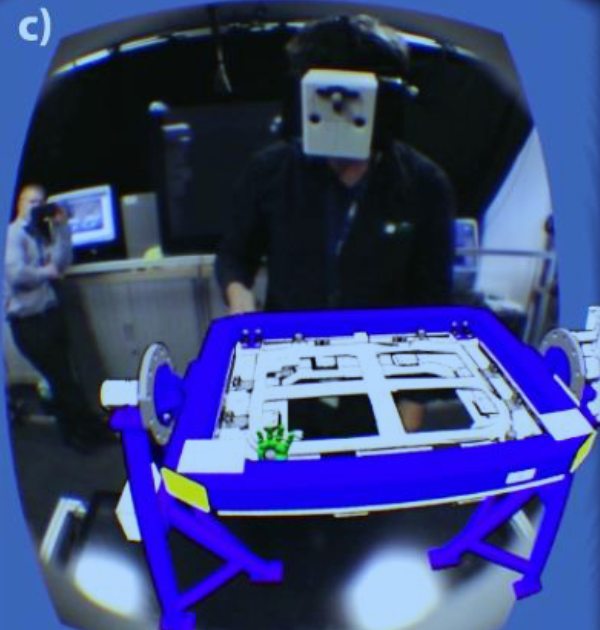
\includegraphics[width=0.35\columnwidth]{figures/category2.png}}
	\subfigure[Interact with virtual objects]{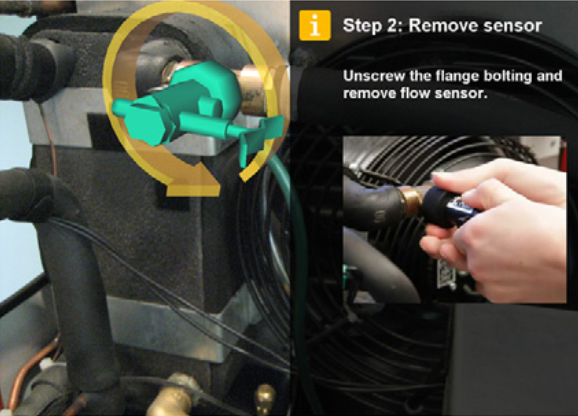
\includegraphics[width=0.51\columnwidth]{figures/category1.png}}
	\captionsource{Two categories of augmented reality training scenarios according to which objects people interact with.}{\cite{gonzalez-franco2016,webel2013}}
	\label{fig:category}
\end{figure}

\subsection{Virtual Objects}
\label{sec:bg:gs:vo}

In the framework depicted in~\cite{nakajima2003}, the camera captures the images of a participant standing in front of a blue screen. The participant uses a "wand" to interact with a virtual environment, where the "wand" can be a finger, a fire extinguisher or other things we have seen in normal life. There is no marker needed to recognize the position and orientation of the "wand".
Luo et al.~\cite{luo2005} developed an AR-based therapy application that was designed for post-stroke finger extension rehabilitation. The application involves both therapists and the patients. During the rehabilitation, the patients need to wear a head-mounted display and an orthosis. The virtual objects prepared by the therapist are mixed with the patient's hand and displayed on the head-mounted display. When the patient is trying to grasp or release the virtual object, the on-site therapist adjusts the assistance provided by the orthosis.
Leblanc et al.~\cite{leblanc2010} compared an AR training method with the traditional methods in the field of straight laparoscopic colorectal skills acquisition training. Traditional methods cost much higher than AR training methods since it uses human cadavers. They conclude that simulator training followed by cadaver training can appropriately integrate simulators into the learning curve and maintain the benefits of both training methodologies.
Nishino et al. present a Japanese calligraphy training system to teach learners how to write better characters~\cite{nishino2011}. It allows the learners to watch and feel the writing techniques of an instructor. More specifically, the training system displays a virtual brush and enables the learners to intuitively master instructor's motor skills through the sense of touch with a haptic device.
Gonzalez-Franco et al.~\cite{gonzalez-franco2016} developed an approach for training in complex manufacturing scenarios, where the virtual objects are projected into real scenes without their real counterparts. The trainers operate on the virtual objects with a wand to teach the trainees.
% This sentence is not needed
In this use case, the interactive targets are the virtual objects.

The methods in this category are usually applied on the fields where the cost or risk of real hands-on experience is too high. For example, a surgeon could use AR to learn how to perform open-heart surgery without risking patients' lives.

\subsection{Real Objects}
\label{sec:bg:gs:ro}

In engineering, especially in the field of machine maintenance and repair, the cost of real hands-on experience is relatively low, but the complexity of the target is very high. In this kind of scenarios, people often use augmented reality technology to show virtual objects as a guide.

Hincapi� et al.~\cite{hincapie2011} demonstrated an AR-based training process to perform maintenance on the body of the RV-10 aircraft. The system overlays virtual objects onto real objects as an instruction. Trainees need to work on the RV-10 aircraft component based on the instructions.
Webel et al.~\cite{webel2011,webel2013} proposed a framework for assembly and maintenance training. The trainees operate on a real machine, while the instructions are shown by overlaying a virtual machine on the real one. In this work, the interactive targets are the real objects, while the virtual ones are shown as the instruction.
Mohr et al.~\cite{mohr2015} present a system which automatically transfers printed technical documentation, such as handbooks, to three-dimensional augmented reality. The proposed system identifies the most frequent forms of instructions found in printed documentation, such as image sequences, explosion diagrams, textual annotations and arrows indicating motion.
Zhu et al.~\cite{zhu2017} aimed to develop a novel registration and tracking technique to establish a navigation system based on augmented reality for maxillofacial surgery. They use a marker to track the relationship between the virtual image and the real object for displaying inferior alveolar nerve bundles in maxillofacial surgery.

AR training scenarios typically involve interacting with objects in the real world, so most of AR training applications fall into the ``Real Objects'' category.
It could be very complex for an AR training system. The modules involved can be categorized into six categories~\cite{wang2016}, i.e., video capture, image analysis and processing, tracking process, interaction handling, instruction information management and rendering. In this proposal, we target in two of them, i.e., instruction information management and rendering.

\section{Training Scenarios}
\label{sec:bg:ts}

Among various fields of augmented reality, we are especially interested in AR's application in training.
Compared with traditional training approaches, trainers trained with AR demonstrate less unsolved errors~\cite{gavish2015_evaluating}.

After reviewing the literature in this area, we categorize the existing works into 3 categories: guidance design, authoring and feedback. The reason why we use the three categories is that guidance is how the trainees accept instructions, authoring is where the guidance comes from while feedback is how the trainees' operations are evaluated and corrected.

Caudell and Mizell~\cite{caudell1992} have proposed the first implementation of a classic AR assembly system by combining head position sensing and real world registration with the HMD, such that a computer-produced diagram, containing pertinent information, can be superimposed and stabilized on a specific position on a real-world object.
Since then, many AR training guidance applications have emerged.
Henderson and Feiner developed a framework to assist conducting military routine maintenance tasks inside an armored vehicle turret~\cite{henderson2009}. The experiment shows that use of AR increases the precision of component locating by 56\% compared with the use of traditional untracked head-up displays (HUDs) and speeds up the task by 47\% compared with standard computer monitors.
Crescenzio et al.~\cite{crescenzio2011} implemented an AR-based maintenance tool for daily inspections of the Cessna C.172P, an airplane often used by flight schools. It superimposes digital replicas of parts and subparts or graphical symbols to attract the operator's attention and guide the technicians through a task. It uses a markerless, feature-based method for HMD registration. What is more interesting is that they also provide an authoring tool for new training material generation. By leveraging the CAD models and existing scanning tools, a trainer can generate new training materials without the knowledge of programming. However, it still requires a lot of efforts to scan the objects to get their 3D structures for tracking purpose.

In order to be more robust, the applications above are designed as task-specific, i.e. not suited for a wide range of different tasks. Practical authoring solution is an popular research topic.
Wang et al.~\cite{wang2010} developed an authoring tool for AR-based examinations. Providing 3D models involved in exam questions, the application generates the AR content and stores it in a separate file that can be shared, edited or imported into an AR interface.
Petersen and Stricker~\cite{petersen2012} reported proof-of-concept systems to create interactive AR manual automatically (for assembly, maintenance, etc.) by segmenting video sequences and live-streams of manual workflows into the comprising single tasks.
However, authoring an AR guidance could be very time-consuming using those tools.
Anderson et al.~\cite{anderson2013} proposed a movement training application that is equipped with a human motion recording tool. They record people's movements and present them in an augmented reality mirror, and the users can see their mirror image as well as the targeting movements in the mirror and follow those movements.
Bhattacharva and Winer~\cite{bhattacharya2015} also presented a method which uses a novel method to capture product assembly steps performed by a user with a depth+RGB camera.
However, they are still not real-time authoring tools, since the content need to be prepared or captured before the training.

Feedback plays an important role in AR training.
There are two types of feedback mechanisms among existing works.
The methods in one type use a intelligent system to evaluate the users' actions.
Nguyen~\cite{kruger2015} proposed an approach to compute the positions of each part of the worker's body with captured input depth images, and analyze the ergonomic scores.
Westerfield et al.~\cite{westerfield2013,westerfield2015} integrated the intelligent tutoring systems (ITSs) with AR interfaces to provide customized instruction to each trainee.
The methods in another type allow supervisors to review and evaluate the task activity performed by the trainees.
Re and Bordegoni~\cite{re2014} presented a monitor system for training, such that supervisors could check the assembly/maintenance activity from a remote display and provide feedback to the users whenever necessary.
To the author's knowledge, there is no existing work that focuses on real-time feedback that could be integrated into the AR training system.

As discussed above, most of the AR training systems are presented as interactive guidances that guide the user through a fixed series of steps.
There are a few issues that need more attention from researchers. First, pre-designed guidances, no matter they leverage an intelligent schema or not, are not suited for a wide range of different tasks, especially for complex ones, since they are always designed as task-specific. Second, lack of collaboration between the trainer and the trainees limits the use of AR training methods in complex tasks, because the trainer is not able to get real-time feedback from the trainees.

We propose a collaborative AR training framework that is not a traditional guidance-like system.
Compared to the existing AR training platforms, the proposed platform has three advantages: 1) It does not require a pre-defined guidance, which makes it suitable to complex tasks; 2) It allows the trainer to collect feedback from the trainees during the training process in real-time; 3) It works with consumer-level devices without dedicated hardware such as powerful graphics.


%======================================================================
\chapter{Details about the Method}
\label{chap:dm}
%======================================================================

In this chapter, we explain the details about our proposed method.
First of all, we give an overview of the framework, and identify the parts that compose the framework. Moreover, some parts have already been studied in our previous work, while some parts need to be explored in the future.
Second, we discuss the communication schema design of our framework.
Third, we demonstrate the for pose estimation of multiple objects, which will be used in our framework.
Last, the limitations of the proposed framework are discussed.

\section{Overview}
\label{sec:dm:ov}

Figure~\ref{fig:ar-training-overview} shows the overview of the proposed AR training framework. It consists of five parts: 1) video capture; 2) video object segmentation; 3) pose estimation; 4) remote rendering; 5) synchronization.
The five parts form a loop that is repeated during the training process.

On the trainer side, the environment is captured as a monocular RGB video. In every loop, a captured frame is sent to the server.
The server is responsible for segmenting the moving objects from the frame. In the segmentation process, the information calculated from previous frames is considered to ensure temporal consistency of the segmentation.
In the pose estimation part, poses of all the moving objects in the current frame are calculated.
With the pose information, the framework is able to render all the moving objects for each trainee, with respect to their respective views.
In the synchronization part, a rendered frame that contains the virtual objects are sent to each client and overlapped on his/her real view.

\begin{figure*}[!htbp]
	\centering
	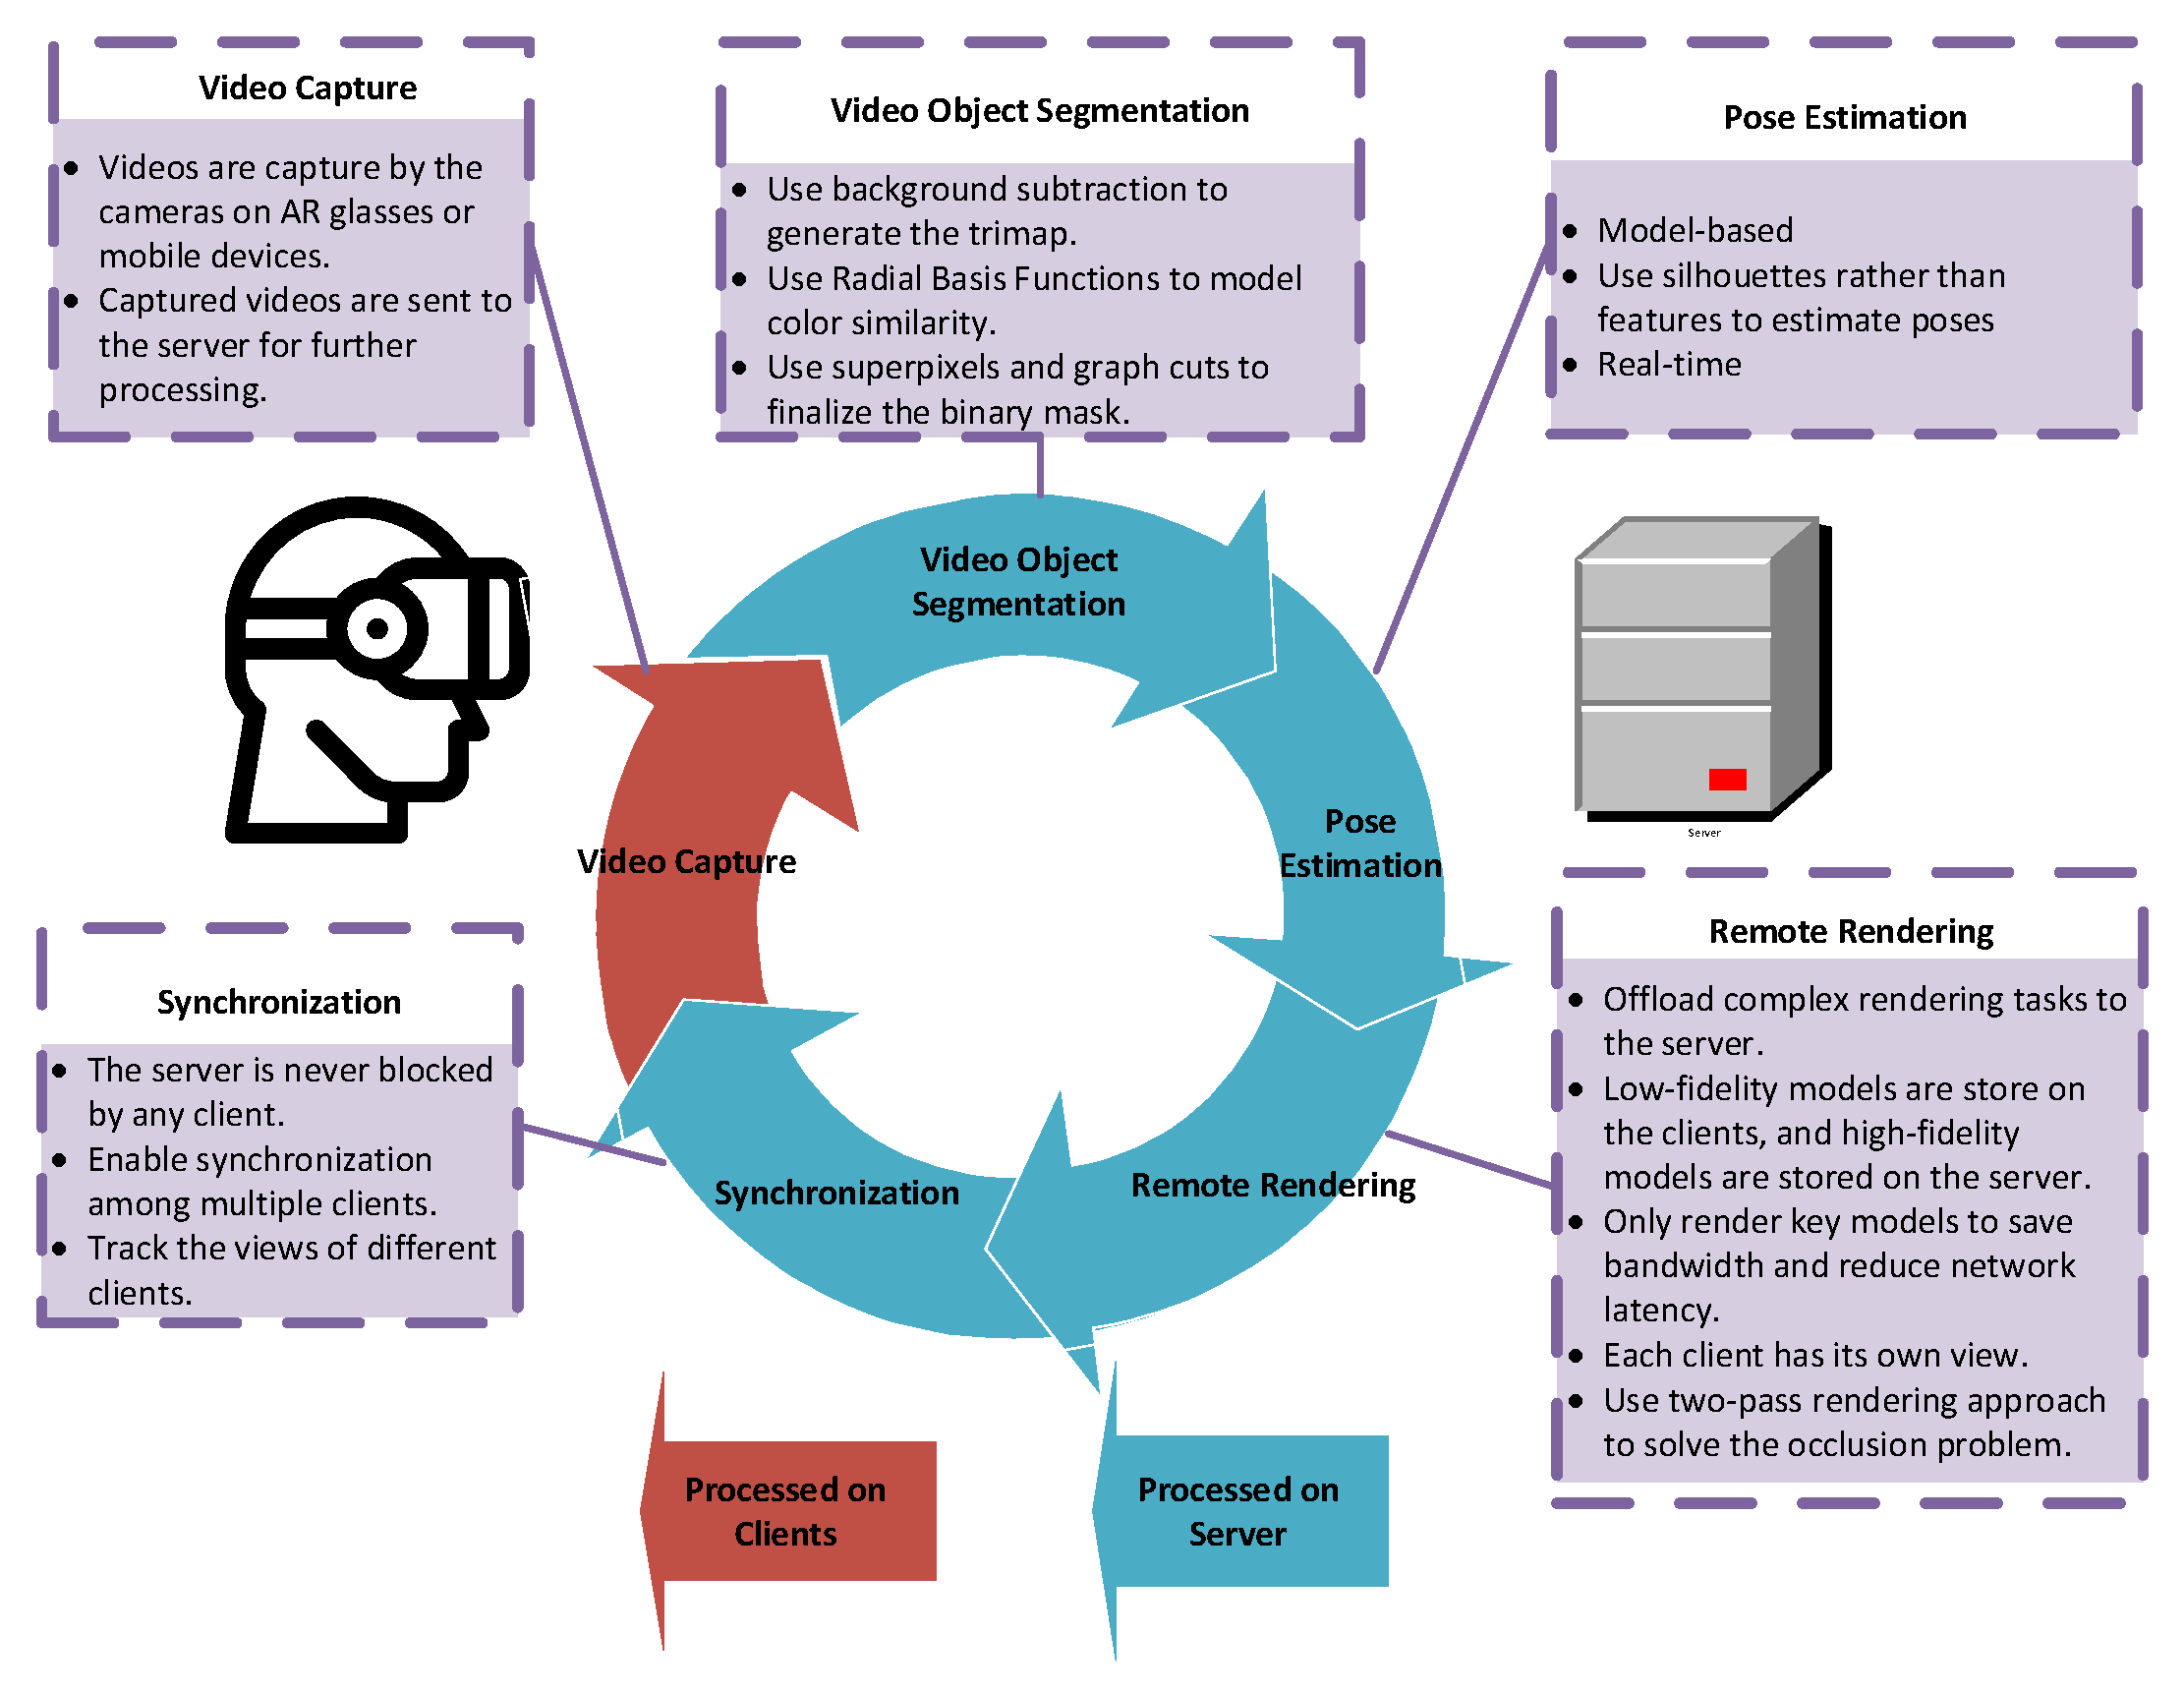
\includegraphics[width=\textwidth]{figures/AR-training-overview.pdf}
	\caption{Overview of the AR training framework. In the circle, the red arrow shows the part performed on the client side, i.e. AR glasses or mobile devices, while the blue arrows show the parts performed on the server side. In this way, the computing cost of the clients is minimized.}
	\label{fig:ar-training-overview}
\end{figure*}

On the trainee side, the procedure is similar.
The environment of every trainee is captured and sent to the server for segmentation and pose estimation.
Then, the moving objects from all the trainees are rendered on the server with respect to the trainer's view.
Last, a rendered frame that contains all the virtual objects are sent to the trainer's AR glasses or mobile devices and overlapped on his/her real view. During this step, virtual objects from different trainees can be marked by colors or markers.

Next, we discuss the details of each part.
% first
First of all, in the video capture part, the videos are captured by the cameras equipped on AR glasses or mobile devices.
The cameras are monocular RGB cameras. In every loop, only one frame is captured.
Moreover, the captured frame is sent to the server for further processing.

% second
Second, in the video object segmentation part, we use background subtraction to generate a trimap that  roughly segments the frame into three regions: a) a definite foreground; b) a definite background; c) a blended region where pixels are considered as a mixture of foreground and background colors.
Then, we use Radial Basis Functions to model color similarity. After this step, every pixel is assigned a value that is the distance between the pixel and the foreground and the background based on a color similarity metric between every pixel in the blended region and the definite regions.
Furthermore, we clearly label each pixel as foreground or background using superpixles and graph cuts.

% third
Third, in the pose estimation part, we use a model-based algorithm that uses silhouettes of objects to estimate poses~\cite{tjaden2016}.
It is a real-time algorithm.
However, the algorithm focus on how to estimating poses with known segmentations. In the original paper, it uses a level-set segmentation method and requires manual initialization of the segmentation.
In our framework, we use the video object segmentation method that we have created, which is also real-time.

% four
Four, AR glasses or mobile devices often has far less powerful graphics capacity than desktop PCs or workstations.
To minimize the computing costs of the clients, we offload the complex rendering tasks to the server.
In the remote rendering method, low-fidelity models are stored on the clients, while high-fidelity models are stored on the server.
Because each client has its own view, the server must render a frame for each client.
To save bandwidth and reduce network latency, the server only renders key models. The rendered frames only contain the key model rendering results.
However, rendering only key models, we have to address the occlusion problem. We use a two-pass rendering approach to solve the problem.

% five
Last, in the synchronization part, we need a mechanism to manage communications between the clients and the server.
It must enable synchronization among multiple clients, and if a client fails to respond, the server must not be blocked.
Furthermore, it has the capacity to track the views of different clients

An advantage of our proposed framework is that, only video capture and relatively simple rendering are performed on the clients, while all the other parts are performed on the server.
In this way, the computing cost of the clients is minimized.

From Figure~\ref{fig:ar-training-overview}, we can see that, to realize the framework, there are three parts that need to be explored.
% first
The first is a video object segmentation part. In the work of Tjaden et al.~\cite{tjaden2016}, they use a level-set segmentation method and requires manual initialization of the segmentation.
Although there are existing automatic algorithms that are able to segment videos without manual initialization~\cite{brox2010,ochs2011,ochs2012,papazoglou2013,wang2015}, some methods are very slow~{brox2010,ochs2011,ochs2012}, some are offline methods that require the availability of the entire video.
Thus, we propose a novel video object segmentation method that is real-time and offers online processing.
This part has been done, and the details about the method can be found in Chapter~\ref{chap:vos}.

% second
The second is a remote rendering method.
AR glasses and mobile devices usually have less graphics capacity, compared to desktop PCs and workstations.
We have proposed a remote rendering method that is compatible with multiple clients to minimize the computing costs of the clients. This work can be found in Chapter~\ref{chap:hrr}.

% third
Last, we need to design and implement a communication schema to manage communications between the clients and the server.
This schema must be able to synchronize the states of different clients and the server.
Moreover, it should have the capacity to track the views of different clients.
This part has not been implemented, and we draw the blueprint of the schema in Section~\ref{sec:dm:csd}.

\section{Communication Schema Design}
\label{sec:dm:csd}

As shown as Figure~\ref{fig-comm-schem}, the system consists of four services: control service, pose estimation service, rendering service and the encoding service.
The control service is responsible for controlling the entire process.
First of all, it sends requests to the pose estimation service to perform pose estimation for each client, including the trainer and all the trainees.
Note that the pose estimation service is a non-blocking service. It receives the video captured from each client independently and updates its estimation result right after receiving every frame from every client. In this way, it maintains a database of the relative pose of each object for each client. Every time it receives the request from the control service, it sends the current database to the control service.

Once the control service gets the result from the pose estimation service, it sends the pose estimation result and the rendering request to the rendering service.
When the rendering service finishes rendering the models of interest for all the clients according to their point of view, it sends back the rendering result to the control service.
Note that the models of interest include the models of the components whose state (i.e. position and orientation) has been changed by the trainer but not changed accordingly by the trainees. In other words, it means the components to which the trainer and the trainees need to pay attention.

Last, the control service sends the rendering result and encoding request to the encoding service. Once the encoding service has accomplished encoding, it sends the encoded frames to each client.
The encoding service is a non-blocking service. The control service does not need to wait for the response from it to continue the process.

\begin{figure*}[!htbp]
	\centering
	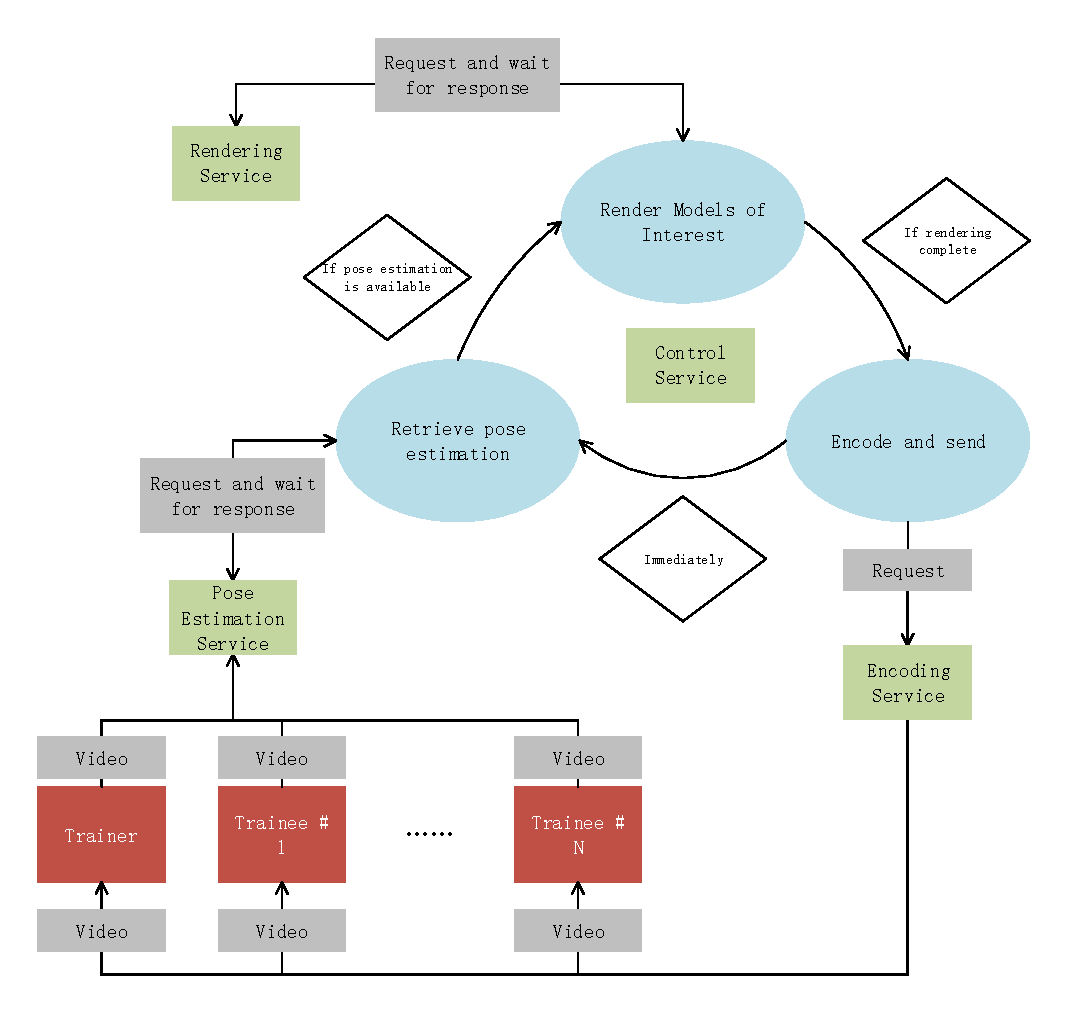
\includegraphics[width=\textwidth]{figures/communication_schema.pdf}
	\caption{Communication Schema}
	\label{fig-comm-schem}
\end{figure*}

As mentioned in Chapter~\ref{chap:hrr}, our remote rendering method includes two types of models: high-fidelity models and low-fidelity models, where the high-fidelity models are stored on the server side while the low-fidelity models are stored on the client side. Thus, even without the rendering service, the clients are able to render the models if they have the basic rendering capacity.
In our schema, the only blocking service is the rendering service. For real-time performance, we set a time limit of $1/30$ second for the rendering service. If it does not accomplish the rendering within the time limit, the control service will send the pose estimation result to the clients and let them do the rendering themselves.

\section{Pose Estimation of Multiple Objects}
\label{sec:dm:pemo}

The first step towards our proposed framework is to estimate the poses of the objects of interest, namely the position and orientation of each object over time.
We use a model-based algorithm to estimate the poses.
With model-based pose estimation algorithms, the 3D structure of the objects of interest must be known beforehand. It is often the case in industrial training~\cite{cremers2007}.

% words need change
Some model-based approaches use edge or point features associated with the 3D models for estimating the pose~\cite{harris1990,vacchetti2004,park2008,kim2010}.
However, there are two major disadvantages with feature-based methods.
First, they struggle with motion blur and are prone to local minima, especially with cluttered backgrounds.
Second, using point-based features also requires the objects' surfaces to be sufficiently textured, which significantly limits the variety of suitable objects.

% words need change
Recently, region-based pose estimation methods have emerged, which are mainly based on statistical level-set segmentation approaches.
The main advantage is that they do not require sufficiently textured objects and only reply on structure of the objects.
However, this category of approaches only work in application scenarios where it is undesirable or even impossible to modify the objects. In other words, they require the objects to be rigid. It is often the case in industrial or manufacturing training.

% words need change
In~\cite{prisacariu2012}, the authors present PWP3D, the first region-based  approach that achieves real-time frame rates (20-25 Hz) using GPUs by solving the pose estimation similar to the variational approach suggested in~\cite{dambreville2010}, but using level-set functions instead of separately integrating over the foreground and background region to simplify computations and make it real-time capable.
Recently, another improved PWP3D version was proposed, which runs at 30 Hz on a mobile phone~\cite{prisacariu2015}.
Tjaden et al. built an algorithm based on PWP3D, which improves convergence properties, especially for rotational motion~\cite{tjaden2016}. Also, the described implementation that uses the GPU only for rendering purposes, and performs the rest computations on the CPU to achieve frame rates of about 50-100 Hz when tracking a single object on a commodity laptop.

Our method uses the work proposed by Tjaden et al.~\cite{tjaden2016} in our pose estimation service, where the object segmentation and pose estimation are performed in an interleaved fashion for each camera image.
However, the approach uses a level-set segmentation method and requires manual initialization of the segmentation, which limits its usage in real applications.
We proposed an automatic video object segmentation method, as described in Chapter~\ref{chap:vos}. In our work, the object segmentations are initialized automatically and it works with multiple objects.
Compared with other state-of-the-art automatic video object segmentation methods, our approach has the advantage that it runs in real-time.
Moreover, the synthetic silhouette that is generated with the models can be used as a ground truth segmentation, which will be used to improve the foreground and background segmentation results.

\section{Limitations}
\label{sec:dm:l}

However, the proposed framework still has several limitations.
First, the 3D models of objects involved in the training must be known beforehand, since the techniques we use in pose estimation are model-based.
The reason why we use a model-based pose estimation method is that this kind of methods are typically more accurate than those approaches that estimate the 3D structure and pose at the same time. Another advantage of using a model-base pose estimation method is that it does not require the presence of markers.
However, our proposed framework aims at training scenarios. In many cases the CAD models are typically known beforehand, such as in manufacturing and assembly tasks.
In some other training scenarios, an extra effort is needed to obtain the 3D structures of the objects involved.
Second, the proposed framework does not work with non-rigid bodies.
For instance, in surgery training, the organs are deformable, and thus, it is not enough to only track the translation and orientation of an organ.

%======================================================================
\chapter{Evaluation}
\label{chap:e}
%======================================================================

To evaluate the developed framework, a skill transfer study will be conducted with the following objectives:

\begin{itemize}
	\item
	to analyze the efficiency of the framework as a training tool for skill transfer, and
	\item
	to compare the performance of trainees with those trained using traditional training methods.
\end{itemize}

The evaluation involves two experimental groups:

\begin{itemize}
	\item
	Two-way AR group: participants are trained using the proposed two-way AR training platform.
	\item
	One-way AR group: participants are trained using the one-way AR training platform.
	\item
	Control group: participants are trained using an instructional video.
\end{itemize}

The experimental task is a mortise-and-tenon assembly task. It requires the participants to assemble the mortise-and-tenon parts together in a proper way. We will recruit 45 participants that are assigned into three groups: participants in the AR group will be trained using the proposed two-way AR training platform, participants in the One-way AR group will be trained using the one-way AR training platform, while those in the control group will be trained using an instructional video.

\section{Procedure}

\subsection{Introduction to the task and procedure}

The experimenter will first explain to the participants the purpose of the experiment - namely to evaluate the different training methods for assembly skills transfer.
The general information about the task will be also given to the participants.
Then they will be told that, after the training, they will be asked to accomplish the task on their own as fast as possible and without errors.

\subsection{Introduction to the training method}

Participants in different groups will be given different introduction to the platform they will use.
Participants in the two-way AR training platform and one-way AR training platform will be given instructions on the tablet PC with a touch screen that would serve as the AR platform. They will also be introduced to the program we will develop to use in the training platform.
Participants in the control group will be told that they would perform the training using an instruction video describing the task.

\subsection{Familiarization with the training platform}

For all the three groups, participants will be asked to familiarize the training platform with a pre-task. The pre-task is a burr puzzle that can be treated as a simplified version of the main task, see Figure~\ref{fig:burr-puzzle}.
The left figure of Figure~\ref{fig:burr-puzzle} shows the components of the burr puzzle, and the right figure shows the assembled status of the burr puzzle.

\begin{figure}
	\centering
	\subfigure[Before assembly]{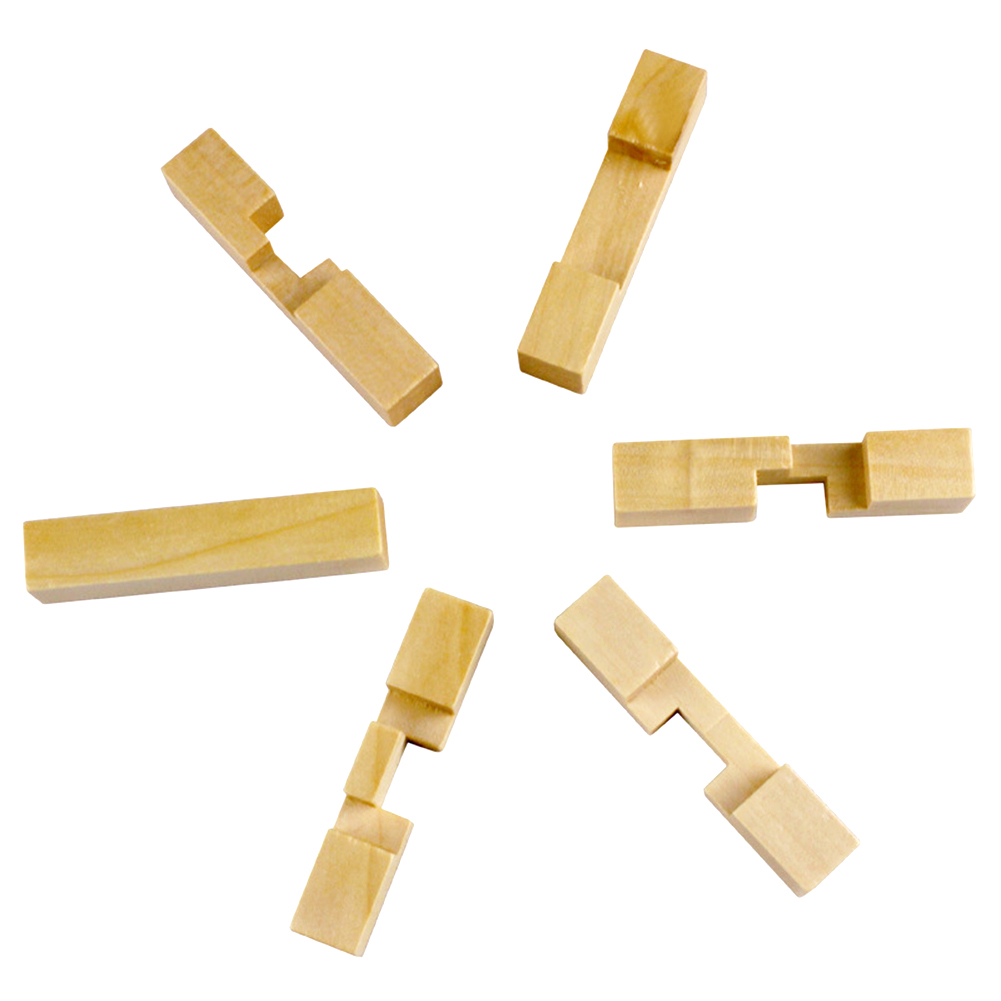
\includegraphics[width=0.35\columnwidth]{figures/burr-puzzle-parts.jpg}}
	\subfigure[After assembly]{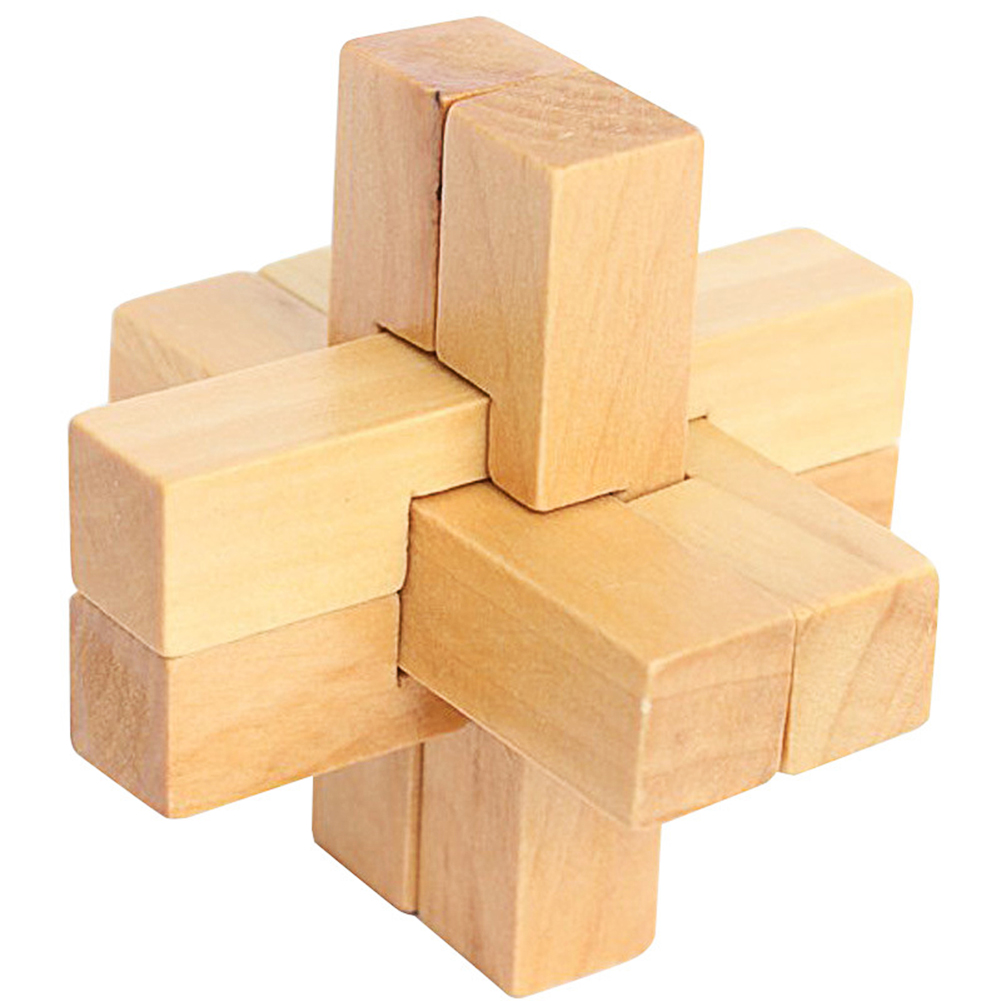
\includegraphics[width=0.35\columnwidth]{figures/burr-puzzle.jpg}}
	\captionsource{Pre-task}{\cite{burr-puzzle}}
	\label{fig:burr-puzzle}
\end{figure}

The participants in all the three groups will be asked to solve the puzzle with the help of the corresponding training method. They will be told that this pre-task is only for them to familiarize the training platform and it is not necessary to solve it if it is too difficult.

\subsection{Training}

After familiarization of the training platform, the training will open with a general explanation of the task, and a reminder to the participants that they will be asked to accomplish the task on their own later.

We choose multi-layer bracket assembly as the mortise-and-tenon task.
The multi-layer bracket is a bracket system used in ancient Chinese architectures.
Figure~\ref{fig:mat-task} demonstrate the multi-layer bracket and its parts. A multi-layer bracket is composed of tens of parts, the parts are connected with each other using mortise-and-tenon joints.

At the beginning of the training, all the parts are detached from each other. The participants will be asked to assemble them with the help of different training platforms.

The participants in the two-way AR group will use the proposed AR training platform, during which the experimenter will act as the remote trainer. The experimenter will perform the task in another room, so that the participants would not to see the experimenter. The participants will follow the live instructions and get the feedback from the experimenter.

The participants in the one-way AR group will use a one-way AR training platform that has pre-defined materials, while the participants in the control group will use an instruction video to learn how to perform the task.

The training time of each participant will be recorded.

\begin{figure}
	\centering
	\subfigure[Multi-layer bracket]{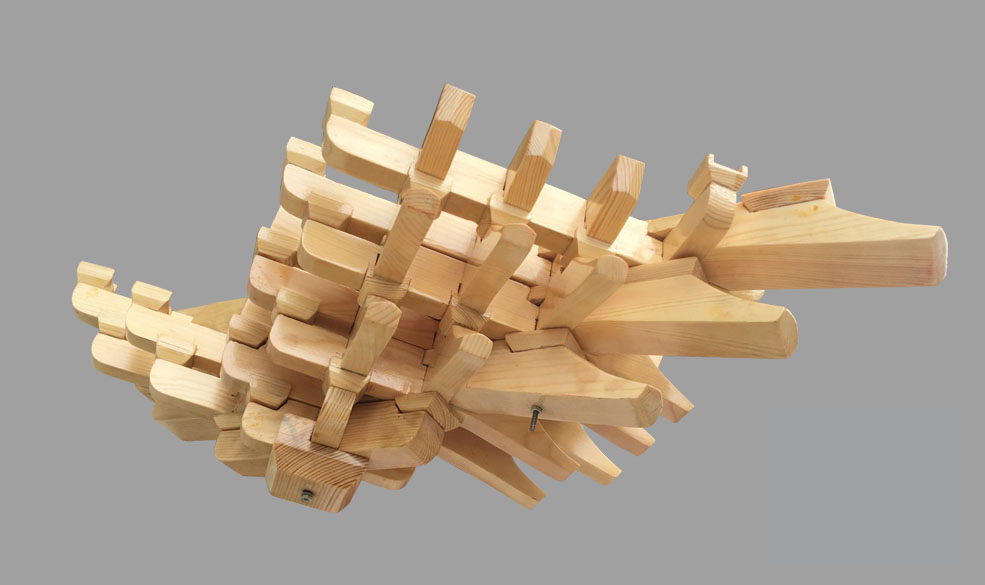
\includegraphics[width=0.35\columnwidth]{figures/bracket.jpg}}
	\subfigure[Parts of the multi-layer bracket]{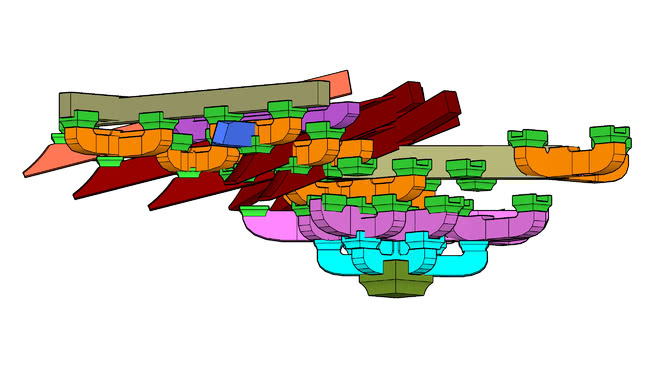
\includegraphics[width=0.35\columnwidth]{figures/bracket-parts.jpg}}
	\centering
	\captionsource{Mortise-and-tenon task}{\cite{ml-bracket-1,ml-bracket-2}}
	\label{fig:mat-task}
\end{figure}

\subsection{Test}

The participants will be asked to perform the task correctly on their own after the training. During the test, if they feel that they could not continue the task, they can ask the experimenter to perform one step for them. However, they will be told that the number of helps from the experimenter indicated the number of solved error, which is one of the measures of their performance.

After the test, we will record the performance time of each participant and inspect the buckets that they assembled to count the number of unsolved errors made by each participant.

\section{Hypothesis}

We devise three null hypothesis to test in the experiment:

\begin{table}[!htbp]
\caption{Hypotheses.}
\label{tab:hypo}
\small{
\begin{tabular}{ll}
\noalign{\smallskip}\hline\noalign{\smallskip}
H\textsubscript{01} & Participants in all the groups have equal performance in performance time \\
H\textsubscript{02} & Participants in all the three groups have equal performance in number of unsolved errors \\
H\textsubscript{03} & Participants in all the three groups have equal performance in number of solved errors \\
\noalign{\smallskip}\hline
\end{tabular}
}
\end{table}

\section{Participants}

45 volunteers will be recruited in the experiment. The number of participants is comparable with similar studies. There are 20 participants in \cite{webel2013}, 24 participants in \cite{wang2010}, 40 participants in \cite{gavish2015}, and 6 participants in \cite{henderson2009}. We will make sure that all the participants do not have experience on the mortise-and-tenon task.

\section{Independent Variables and Dependent Measures}

The experiment will be conducted with three independent variables: training method. It has three levels: two-way AR training platform, one-way AR training platform, and instruction video.

In the experiment, we will collect three types of data: performance time, number of solved errors, and number of unsolved errors.
The performance time indicates the time period during which the participants accomplish the task.
Number of solved errors is the numbers of helps the participant got from the experimenter.
Number of unsolved errors indicates the number of errors on the finished product.

\section{Analysis}

After the experiment, we can calculate the mean values for all the three measures and groups. However, to understand the result statistically, we use analysis of variance (ANOVA) to interpret our experiment results.

Since there is only one independent variable, training method, we use one-way ANOVA test to investigate the effect of the factor. We compare the $p$-value to a significance level to decide whether the null hypothesis should be rejected. We choose a significance level of 0.05.

%======================================================================
\chapter{Video Object Segmentation}
\label{chap:vos}
%======================================================================

In this section, we present a method for extracting foreground objects from video and its application to content-aware video compression. Our method uses trimaps inferred from background subtraction to represent the foreground-background relationship. The appearance of foreground and background are modelled with Radial Basis Functions initialized from the background substraction step. Finally, Graph Cuts are used to compute a binary mask. Our method is fully automatic, fast, and does not make restrictive assumptions about object motions. In experiments on standard data sets, the proposed approach achieves comparable results to state-of-the-art video object segmentation methods but our method is much faster. We also demonstrate an application of the proposed method to content-aware video compression.

\section{Introduction}
\label{sec:vos:i}

Video object segmentation is the process of separating foreground objects from the background in a video~\cite{papazoglou2013}. A wide range of applications benefit from the progress of video object segmentation, e.g. robot-object interaction, recognition, and video compression.

A variety of methods have been proposed to address the task~\cite{papazoglou2013,ma2012,wang2015,brox2010,taylor2015}. Most methods use motion cues to initialize the object segmentation.
A common method for motion detection is  background subtraction with mixture of Gaussians~\cite{kaewtrakulpong2002,zivkovic2004}. This technique models each pixel indepedently as a mixture of Gaussians, but as it detects motion in each frame independently, the results lack completeness and temporal persistence.
In this paper, we address this shortcoming by modelling the appearance of objects from motion. 

Our proposed method treats moving pixels as a partial segmentation of objects and builds the appearance model for them, see Section~\ref{sec:vos:m:csc}. With the appearance model, those pixels that are not moving can successfully be classified as foreground or background to form a more complete segmentation. We model appearance with Radial Basis Functions (RBF) as described in Section~\ref{sec:vos:m:csc}, an approach commonly used in interactive editing for selection propagation~\cite{li2010,tao2012}. We adapt the technique of Tao and Krishnaswamy~\cite{tao2012} but use motion detection instead of user selection to initialize the models.
 
Moving pixels obtained with background subtraction approaches may be not just incomplete, but also contain pixels from the background. This is mainly caused by shadows and noise. The consequence is that the computed segmentations are likely to cover regions that are not part of the foreground. We address this mis-classification with modelling background appearance and optimizing the classification. We use Graph Cuts~\cite{greig1989,boykov2004} to optimize the foreground and background classification based on the appearance model. To accelerate the computation, we divide frames into regions that contain one object each (see Section~\ref{sec:vos:m:tg}), and oversegment those regions with a fast superpixel method~\cite{siva2014} before classification (see Section~\ref{sec:vos:m:fbl}).

We evaluate our video object segmentation approach on a common dataset~\cite{f-li2013} in Section~\ref{sec:vos:e:ds}. Our evaluation demonstrates that our approach achieves comparable results to two state-of-the-art approaches, but our approach is on-line and is $10-200 \times$ faster than these methods.

The major contribution of our work is a fast on-line video object segmentation method that takes both motion and appearance of objects into account. We propose a novel integration of RBF appearance modelling and background subtraction through a Graph Cuts optimization on superpixels. We use local modelling to accelerate segmentation by dividing frames into regions that contain one foreground object each which greatly reduces the number of pixels to be processed. In Section~\ref{sec:vos:cavc}, we propose an application of our on-line approach for compressing videos with compression quality adapted to foreground and background. The video object segmentation allows us to reduce the quality of the background by pre-processing it with a bilateral filter before compression while foreground objects are compressed as is by the compression scheme. We use H.264 coding.

\section{Background}
\label{sec:vos:bg}

A large number of methods have been proposed for extracting moving objects from an image sequence, using motion, depth, appearance, or a combination of these cues.
Among those, motion is used most frequently as cues for object extraction~\cite{graciela2013}, and many approaches use
background subtraction to this end~\cite{zeng2007,colombari2007}.
Classic background subtraction methods model the appearance of the background at each pixel and label the pixel that change rapidly to be foreground~\cite{jain1979,kaewtrakulpong2002,zivkovic2004}. These methods typically assume a stationary or slowly panning camera.
More recently, optical flow is also used~\cite{ma2012,papazoglou2013,zhang2013,wang2015}.
The motion estimation algorithms typically provide pixel-wise labeling and errors are inevitable even when using state-of-art algorithms.
To obtain robuster masks with semantic meaning, energy minimization is often used~\cite{papazoglou2013}.
Optical flow usually provides more motion cues than background subtraction (e.g. pixel correspondence across frames), but in general, is much slower than background subtraction methods.
Our approach is closely related to tracking. We infer trimaps from detected motion to coarsely separate foreground from background, which is different from other methods based on motion cues~\cite{papazoglou2013,wang2015}.

With the advances in computational power of modern PCs and the progress of fast superpixel methods, the use of superpixels as units of object extraction is increasingly becoming popular~\cite{papazoglou2013,wang2015,ochs2011}. Instead of naive superpixel voting schemes, researchers often use some optimization approaches to decide if a superpixel belongs to the foreground or the background~\cite{papazoglou2013,wang2015,ochs2011}. However, most of the superpixel methods are computationally intensive, which prevents their use in real-time video object extraction~\cite{achanta2012}. A fast superpixel method was proposed by Siva and Wang~\cite{siva2014}. It is based on seam carving and dynamic programming, and it achieves real-time performance in low resolution videos. We adapt this method and further accelerate the computation of superpixels by only segmenting the regions within the bounding boxes of foreground objects into superpixels.

Several video object extraction methods track points over the image sequences and then cluster the resulting point trajectories pairwise or in triplets~\cite{brox2010,ochs2011,ochs2012}.
The advantage of employing point tracking is the capacity of handling videos where moving objects are stationary in a number of frames.
The underlying assumption induced is that the objects are rigid so that all object points move according to a single translation~\cite{brox2010,ochs2011}, while the work of Ochs et al.~\cite{ochs2012} assumes a single similarity transformation. This assumption makes these methods not applicable to non-rigid objects.
The methods produce a sparse labeling in each frame, and superpixels are taken into account when turning the point trajectories into dense regions.
These methods are also able to handle partial occlusion but the drawback is that they are very slow (in the order of minutes per frame).

The work by Lee et al.~\cite{lee2011} shows the potential of using shape matching in object extraction.
The method first identifies object-like regions in any frame~\cite{endres2010}, followed by computing a series of binary partitions among those candidate regions to discover groups of shapes with persistent appearance and motion.
The drawbacks of this method include that it requires pre-processing identifying all object-like regions beforehand, it is very slow (in the order of minutes per frame), and it is not applicable to stationary or occluded (in some frames) foreground objects.

Depth information has been demonstrated to be robust to environment changes such as illumination change, dynamic backgrounds, and camera motion~\cite{dahan2011,taylor2015}.
The work of Taylor et al.~\cite{taylor2015} infers depth layers from occlusion information. This gives it the capacity to be used outdoors and ensures that it is robust to occlusion and disocclusion. However, the method takes around 30 seconds for a VGA image on a standard desktop.

The works of Papazoglou and Ferrari~\cite{papazoglou2013} and Wang et al.~\cite{wang2015} are closely related to ours. Papazoglou and Ferrari~\cite{papazoglou2013} use optical flow as the motion cues. After generating a coarse segmentation, Graph Cuts are used to minimize an energy function containing an appearance term and smoothness terms. In this paper, we propose a novel algorithm based on Radial Basis Functions to model the appearance and estimate how close it is from a pixel to foreground or background, considering the neighbouring frames. We also use Graph Cuts to obtain the final masks.

Many modern approaches offer offline processing to recognize objects in videos~\cite{papazoglou2013,ma2012,wang2015,brox2010}. The requirement of the availability of the entire video limits those methods in processing long sequences.
In contrast, our method is online and offers processing in "streaming", which gives it the capacity to handle longer videos and integrate with other online applications.

\section{Method}
\label{sec:vos:m}

Our method consists of three steps: (1) trimap generation, (2) color similarity calculation, (3) foreground-background labelling. Figure~\ref{fig-overview} illustrates the overview of the proposed pipeline. First, motion is detected with the background subtraction method, followed by blob analysis to generate trimaps. Second, the appearance model is built with Radial Basis Functions, where sampling is done in different regions of the trimap for foreground and background respectively. With knowing how close a pixel is to the foreground or the background according to its color, we produce evidence maps. To enhance the spatial and temporal persistency, we smooth the maps with a bilateral filter kernel. Third, using Graph Cuts, we are able to generate a binary mask by minimizing an energy function. Next, we present the detail of these steps.

\begin{figure*}
	\centering
	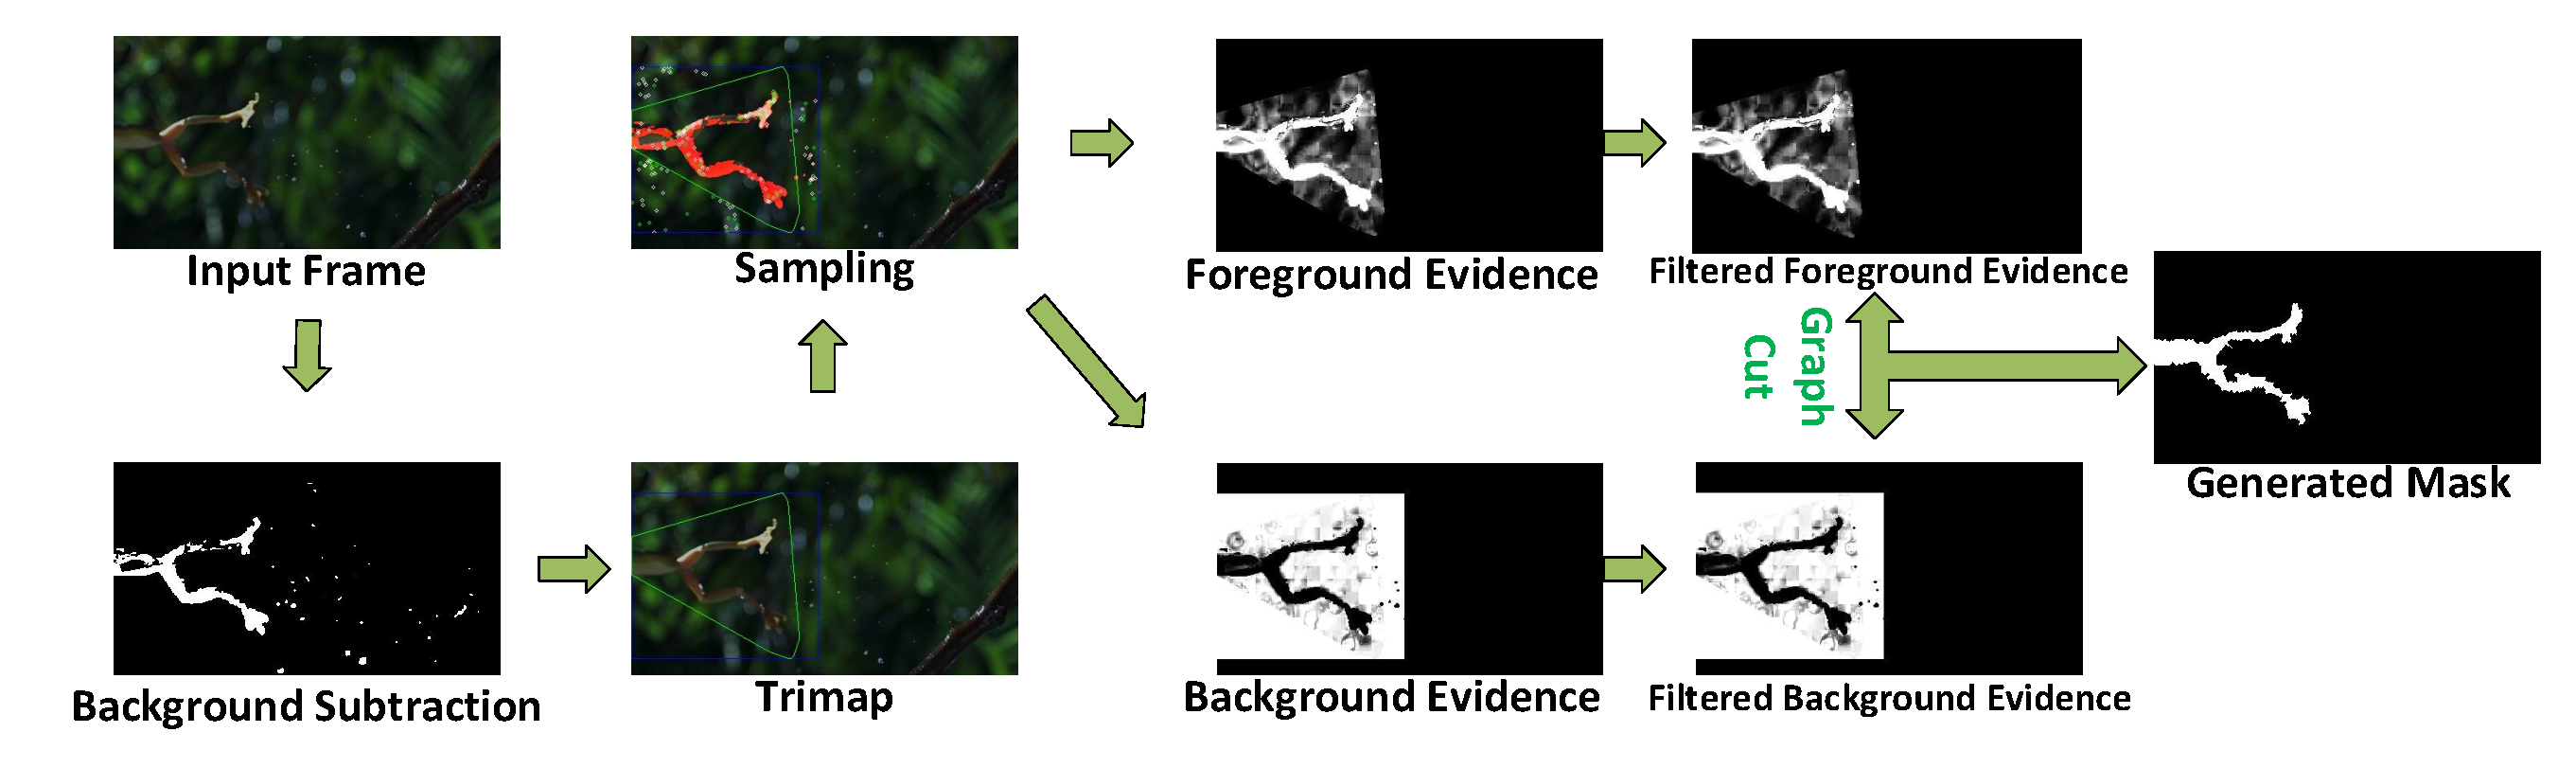
\includegraphics[width=\textwidth]{figures/overview.pdf}
	\caption{Overview of the proposed video object segmentation method. The images are a frame from the dataset SegTrack v2~\cite{f-li2013}.}
	\label{fig-overview}
\end{figure*}

\subsection{Trimap Generation}
\label{sec:vos:m:tg}

\textbf{Background subtraction.}
We begin by computing background subtraction frame by frame using effective  mixture of Gaussians algorithms~\cite{kaewtrakulpong2002,zivkovic2004} according to a comparison~\cite{sobral2014} of various background subtraction methods. We employ the implementations of the two algorithms MOG and MOG2 in OpenCV. After background subtraction, we perform a median filter of kernel size 3 to reduce noise, see Figure~\ref{fig-trimap}(b).

\textbf{Blob analysis.}
After obtaining moving pixels in the background subtraction step, we apply closing morphological transformation to group them. We perform a dilation step followed by an erosion in the binary labelling of the image as it is typically used to close small hole inside the foreground objects.
The purpose of grouping moving pixels is to reduce isolated moving pixels.
Then the convex hulls of blob contours are calculated. The contours are found using Suzuki's algorithm~\cite{suzuki1985} while convex hulls are calculated using Sklansky's algorithm~\cite{sklansky1982}. The bounding boxes are then computed from the convex hulls, see Figure \ref{fig-trimap}(c).

We base our trimap generation on the contours and bounding boxes of the blobs of moving pixels.
A trimap is a partition of images into three regions: a definite foreground, a definite background, and a blended region where pixels are considered as a mixture of foreground and background colors.
More specifically, moving pixels obtained using background subtraction serve as the definite foreground, while the pixels inside the bounding box and outside of the convex hull are treated as definite background.
Those pixels inside the convex hull but not recognized as moving pixels are the blended region.
Such a trimap is established for each blob and segmented individually.
Because in some cases, background subtraction generates trimaps smaller than the actual size of objects, we expand the areas of the convex hulls and bounding boxes by a ratio $r$ such that $A^{*}=r\cdot A$, where $A$ and $A^{*}$ are the areas before and after expansion respectively, see Figure~\ref{fig-trimap}(d).  In our implementation, we typically use $r=2$.

\begin{figure}
	\centering
	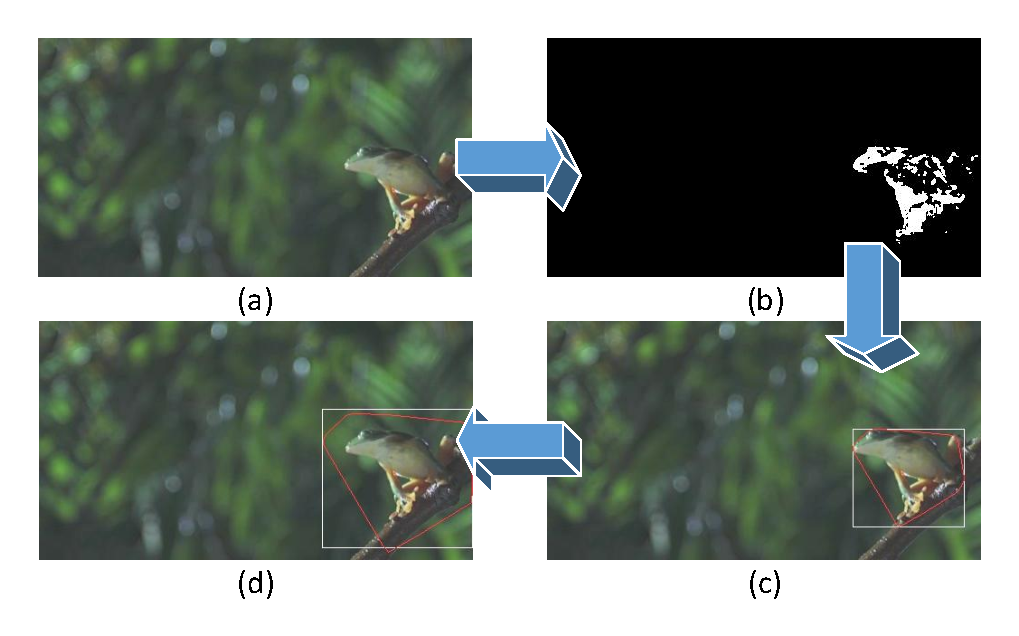
\includegraphics[width=3.3in]{figures/trimap.pdf}
	\caption{Trimap generation. (a) Original frame. (b) Background subtraction result. (c) Convex hull (red) and bounding box (white) of the blob. (d) Convex hull (red) and bounding box (white) after expansion. The images are a frame from the dataset SegTrack v2~\cite{f-li2013}.}
	\label{fig-trimap}
\end{figure}

\subsection{Color Similarity Calculation}
\label{sec:vos:m:csc}

The goal of this stage is to estimate the distance of a pixel to the foreground and the background based on a color similarity metric between every pixel in the blended region and the definite regions.

\textbf{Radial Basis Functions}
Li et al.\ described in detail a method using Radial Basis Functions (RBF) to propagate user edits in image matting \cite{li2010}.
Similar to \cite{li2010}, we use RBF to account for all the pixels within the definite foreground or the background regions.
However, we define the RBF in the three-dimensional color space where each pixel $i$ is represented by its feature vector $\mathbf{f}_{i}$.
The method samples the foreground pixels and the background pixels, respectively, and computes the coefficients of the Radial Basis Functions subject to interpolation constraints using a linear solver.
With $G$ representing all foreground or background pixels, we formulate the interpolation constraints as a least-square energy function, 
\begin{equation}
\label{equ-rbf-ef}
\sum_{i\in E}{(1-h(\mathbf{f}_{i}))^2}
\end{equation}
where $E\in G$ is the subset of all definite foreground or background pixels, and $\mathbf{f}_{i}$ is the color vector of pixel $i$.
$h(\cdot)$ is the RBF centered at the pixels in $B\in G$, where $B$ is another subset of $G$.
To allow {\em soft} interpolation and to gain computational efficiency, we define that $|B| < |E|$, where $|\cdot|$ counts the number of pixels in a set. We choose to sample the set $E$ to have twice the size of $B$. Let
\begin{eqnarray}
\label{equ-rbf}
h(\mathbf{f})&=&\sum_{i\in B}{a_{i}\phi(||\mathbf{f}-\mathbf{f}_{i}||)} \\
\mbox{with}\;\;
% \label{equ-basis}
\phi(r)&=&exp(-\sigma *r^2) \nonumber
\end{eqnarray}
where $\mathbf{f}$ is any point in the color space, $a_{i}$ are the unknown coefficients, $\phi(\cdot)$ is some pre-defined radial basis, and $\sigma$ controls the smoothness of the Gaussian bases~\cite{li2010}.

The coefficients $a_{i}$ represent the importance of a color being similar to a color within the set $B$. Equation~\ref{equ-rbf} directly estimates the similarity of a color to all the colors in the foreground or the background regions. Pixels with the value of 1 are most similar to the corresponding definite region while pixels with the value of 0 represent dissimilar colors. As subsets are sampled from definite regions and Equation~\ref{equ-rbf-ef} is over-determined, the values of pixels may be greater than 1 or less than 0, but we clip the values to $[0,1]$.

The reason why we use a subset $E\in G$ instead of $G$ to construct Equation~\ref{equ-rbf-ef} is to accelerate the computation because each pixel is costly due to the use of the linear solver to compute the RBF~\cite{tao2012}.
%With high-resolution videos, the number of pixels in $G$ can be large, and there is no need to use all pixels in foreground and background regions, respectively, as long as consistent results can be maintained. With too few samples, the RBF behaves inconsistently and sampling plays a critical role in determining the quality of the function. As discussed by Tao and Krishnaswamy~\cite{tao2012}, if pixels are sampled randomly, noise affects the results. Figure \ref{fig-image-matting} shows an example of computing color similarity with RBF.

\begin{figure}
	\centering
	\subfigure[Input Image and Strokes]{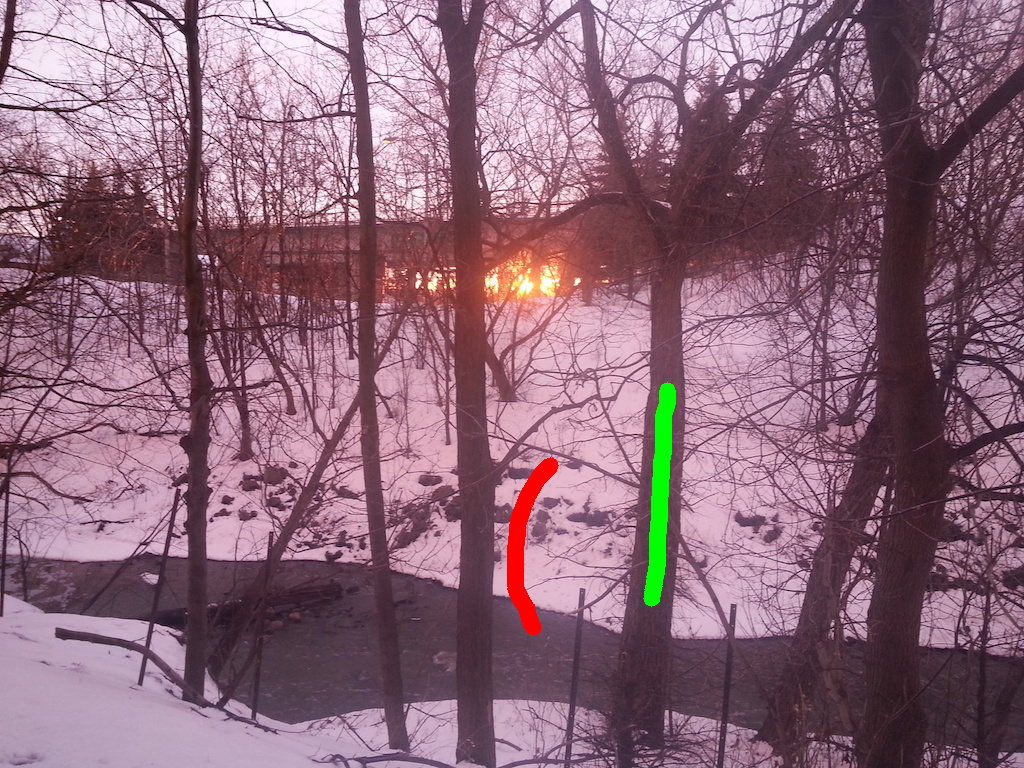
\includegraphics[width=0.35\columnwidth]{figures/img_selects.png}}
	\subfigure[Output Image]{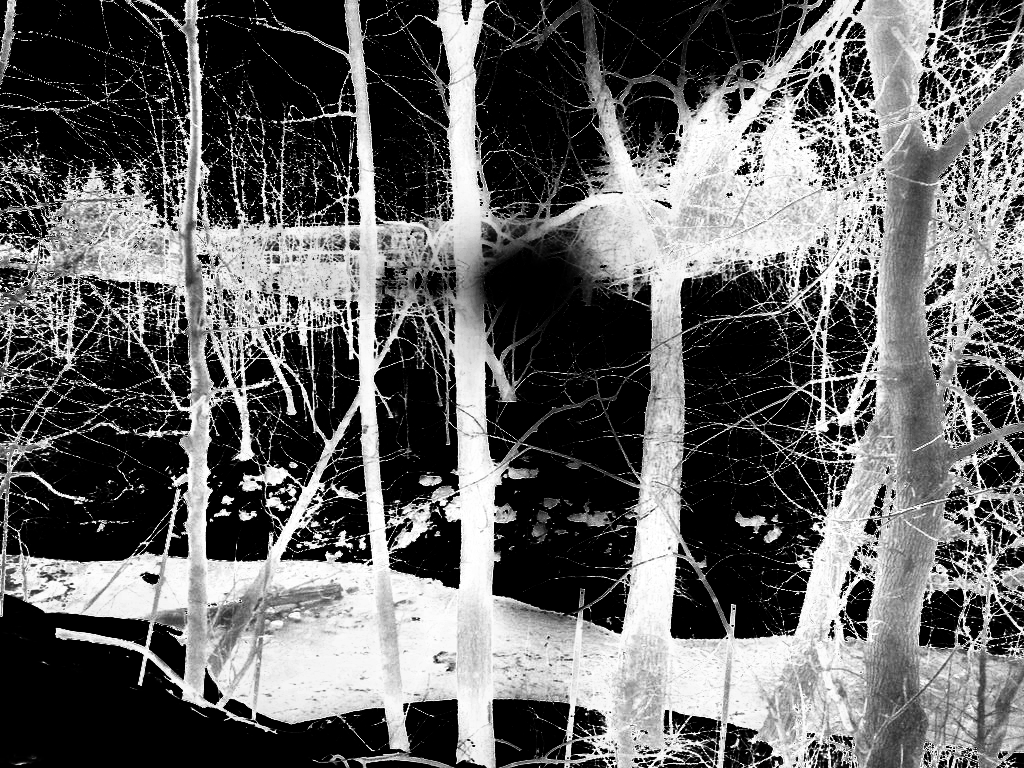
\includegraphics[width=0.35\columnwidth]{figures/sMap.png}}
	\caption{An example of computing color similarity with RBF. (a) The two strokes specifies pixels having similarity 1 (green) and 0 (red). (b) The resulting RBF is applied on every pixel.}
	\label{fig-image-matting}
\end{figure}

Moreover, we adapt the method used by Tao and Krishnaswamy~\cite{tao2012} to sample the definite foreground or background regions using importance sampling rather than random sampling. Our goal is to reduce the number of samples needed while maintaining consistent results.
In our application, we use 27 clusters, 54 radial basis functions and 108 terms in Equation~\ref{equ-rbf-ef}.

\textbf{Foreground and background evidence.}
Assume that $F$ is the set of definite foreground pixels, $B$ is the set of background pixels, and $D$ is the set of blended pixels. We define the evidence of the $i^{th}$ pixel to be the foreground $e_{f}(\mathbf{f}_{i})$ as
\begin{equation}
	\label{equ-ef}
	e_{f}(\mathbf{f}_{i})=
		\begin{cases}
			1, & \text{if } i\in F\\
			clip(h_{f}(\mathbf{f}_{i})), & \text{if } i\in D\\
			0, & \text{if } i\in B
		\end{cases}
\end{equation}
where $\mathbf{f}_{i}$ is the color vector of the $i^{th}$ pixel, $h_{f}(\mathbf{f}_{i})$ is the RBF to the foreground region and $clip(\cdot)$ clips a value to the range $[0,1]$. Similarly, the preference of the $i^{th}$ pixel to be the background $e_{b}(\mathbf{f}_{i})$ as
\begin{equation}
	\label{equ-eb}
	e_{b}(\mathbf{f}_{i})=
		\begin{cases}
			1, & \text{if } i\in B\\
			clip(h_{b}(\mathbf{f}_{i})), & \text{if } i\in D\\
			0, & \text{if } i\in F
		\end{cases}
\end{equation}
where $h_{b}(\mathbf{f}_{i})$ is the RBF to the background region.

\textbf{Evidence smoothness}
For some videos, the temporal persistence of background subtraction methods is poor; therefore, the RBF of the same object can vary greatly from frame to frame.
To alleviate this problem, we add an extra smoothing step to the evidence computation. We use a filter with a cubic kernel in the spatial and temporal domain, and smooth the foreground evidence and the background evidence separately.
The smoothed evidence of pixel $p$ is a weighted sum of the set of its neighbouring pixels $\Omega^{+}$, where $\Omega^{+}$ is the window centered in $p$.
However, when the algorithm processes the $t^{th}$ frame, the frames after the $t^{th}$ frame are not available; therefore, only half of $\Omega^{+}$ actually have an effect, denoted as $\Omega$. The smoothed foreground evidence $e_{f}^{*}$ is represented as
\begin{eqnarray}
	e_{f}^{*}(p)&=&\frac{\sum_{q\in\Omega}{e_{f}(q)\cdot w_{p,q}}}{\sum_{q\in\Omega}{w_{p,q}}} \;\; \mbox{where} \label{equ-w} \\
	w_{p,q}&=&exp(-\frac{(p_{x}-q_{x})^2+(p_{y}-q_{y})^2}{2\sigma_{d}^{2}}-\frac{||\mathbf{f}_{p}-\mathbf{f}_{q}||^2}{2\sigma_{r}^2}) \nonumber
\end{eqnarray}

In Equation~\ref{equ-w}, $p_{x}$ and $q_{x}$ are $x$ coordinates of pixels $p$ and $q$, while $p_{y}$ and $q_{y}$ are $y$ coordinates of pixels $p$ and $q$; $\mathbf{f}_{p}$ and $\mathbf{f}_{q}$ are the color vectors of these pixels.
The variances $\sigma_{d}^{2}$ and $\sigma_{r}^2$ control the degree of smoothness. By increasing $\sigma_{d}^{2}$ and $\sigma_{r}^2$, the evidence becomes smoother. We set $\sigma_{d}^{2}=1$ and $\sigma_{r}^2=1$, which are the same weights as in a bilateral filter. The filter performs smoothing while preserving dissimilarity between pixels far away or with greatly distinct colors.

\subsection{Foreground-background Labelling}
\label{sec:vos:m:fbl}

\textbf{Superpixels.}
We oversegment the $m^{th}$ trimap in the $t^{th}$ frame into superpixels $\mathcal{S}_{m}^{t}$, which greatly reduces computational and memory costs.
We use the method proposed by Siva and Wong~\cite{siva2014}, which is a seam carving approach to superpixel generation and yields results with grid structure. This method is proven to be faster than most of the existing approaches, and can achieve accuracies close to the state-of-the-art superpixel generation algorithms, e.g. SLIC~\cite{achanta2012}.

\textbf{Graph Cuts.}
The problem of segmentation can be considered as an energy minimization problem.
%% Greig et al.~\cite{greig1989} were first to discover that powerfull min-cut/max-flow algorithms from combinational optimization can be used to minimize certain important energy functions in computer vision.
%% As illustrated in Figure \ref{fig-graphcut}, they constructed an undirected graph $\mathcal{G}=<\mathcal{V},\mathcal{E}>$ that is defined as a set of nodes (vertices $\mathcal{V}$) and a set of undirected edges ($\mathcal{E}$) that connect those nodes. Each edge $e\in\mathcal{E}$ in the graph is assigned a nonnegative weight (cost) $w_{e}$. There are also two special nodes called terminals: source and sink. A cut is a subset of edges $\mathcal{C}\in\mathcal{E}$ such that the terminals become seperated on the induced graph $\mathcal{G}(\mathcal{C})=<\mathcal{V},\mathcal{E}\backslash\mathcal{C}>$. Graph Cut is to find minumum $W(\mathcal{C})$ where

%% \begin{equation}
%% W(\mathcal{C})=\sum_{e\in\mathcal{C}}{w_{e}}
%% \end{equation}

%% \begin{figure}
%% 	\centering
%% 	\includegraphics[width=3.3in]{imgs/graphcut.jpg}
%% 	\caption{Graph Cut.}
%% 	\label{fig-graphcut}
%% \end{figure}
We use graph cuts in the minimization and represent the superpixels $\mathcal{S}_{m}^{t}$ as the nodes $\mathcal{V}$ in a graph with an edge to every neighbouring superpixel. A neighbouring superpixel is defined as superpixel that borders the superpixel under consideration, either horizontally or vertically. The two terminals in the graph cut represent the labels of foreground and background. Therefore,
\begin{equation}
E(\mathcal{L})=\sum_{i\in\mathcal{S}}{D_{i}(\mathcal{L}_{i})}+\sum_{(i,j)\in\mathcal{N}}{V_{i,j}(\mathcal{L}_{i},\mathcal{L}_{j})},
\end{equation}
where $\mathcal{L}=\{\mathcal{L}_{i}|i\in\mathcal{I}\}$ is a labelling of superpixels $\mathcal{S}$. $D_{i}$ is a data penalty function, $V_{i,j}$ is an interaction potential, and $\mathcal{N}$ is a set of all pairs of neighbouring superpixels.
For simplicity, we discard the superscript and subscript of the notation $\mathcal{S}_{m}^{t}$.
$D_{i}$ denotes individual label-preferences of superpixels to be foreground or background.
Interaction potentials $V_{i,j}$ encourages spatial coherence by penalizing segmentation between non-edge superpixel pairs.

$D_{i}$ is represented by the sum of evidence for pixels to be foreground or background.
\begin{equation}
	D_{i}(\mathcal{L}_{i})=
	\begin{cases}
		\sum_{p\in\mathcal{S}_{i}}e_{b}(\mathbf{f}_{p}), & \mathcal{L}_{i}=1\\
		\sum_{p\in\mathcal{S}_{i}}e_{f}(\mathbf{f}_{p}), & \mathcal{L}_{i}=0
	\end{cases}
\end{equation}
where $\mathcal{S}_{i}$ is the $i^{th}$ superpixel, $p$ is a pixel within the superpixel $\mathcal{S}_{i}$, $\mathbf{f}_{p}$ is the color vector of the pixel $p$, and $e_{f}$ and $e_{b}$ are define in Equation~\ref{equ-ef} and Equation~\ref{equ-eb}, respectively. $V_{i,j}$ is represented by the Euclidean distance between average color vectors of two superpixels, i.e.,
\begin{equation}
	V_{i,j}(\mathcal{L}_{i},\mathcal{L}_{j})=
	\begin{cases}
		dist(i,j), & \mathcal{L}_{i}\neq\mathcal{L}_{j}\\
		0, & \mathcal{L}_{i}=\mathcal{L}_{j}
	\end{cases}
\end{equation}
where $dist(i,j)$ computes the Euclidean distance between average color vectors of the $i^{th}$ and $j^{th}$ superpixels. The output segmentation is then the labelling that minimizes
\begin{equation}
	\label{equ-mini}
	\mathcal{L}^{*}=\argmin_{\mathcal{L}}E(\mathcal{L}).
\end{equation}
We use the method proposed by Boykov and Kolmogorov \cite{boykov2004} to solve Equation \ref{equ-mini}.

\section{Evaluation}
\label{sec:vos:e}

\subsection{Dataset}
\label{sec:vos:e:ds}

We evaluate our method on the dataset SegTrack v2~\cite{f-li2013}. SegTrack v2 is a video segmentation dataset with full pixel-level annotations on multiple objects at each frame within each video.
It contains 14 videos, including videos captured by either static cameras or moving cameras. We use the five videos with static cameras (birdfall, frog, hummingbird, bird\_of\_paradise and penguin).
The ground truth of the videos hummingbird and penguin are split up, with each object labelled separately. In those cases, we combine the separate labels of the ground truth together to obtain a ground truth with labels for all objects.

% \subsection{Measurements}
% \label{measurements}

We quantify performance with the F-Measure~\cite{sobral2014} based on the amount of true positives (TP), true negatives (TN), false positives (FP) and false negatives (FN). The F-Measure is defined as the harmonic mean of precision and recall, where $Precision = \frac{TP}{TP+FP}$ and $Recall = \frac{TP}{TP+FN}$, and hence the F-Measure
\begin{equation}
\label{equ-fm}
FM = \frac{2*Precision*Recall}{Precision+Recall}.
\end{equation}
where the F-Measure ranges from $0$ to $1$, with value $1$ representing the ground truth segmentation.

%% In the context of video object segmentation, both precision and recall are important measures, i.e. the fraction of correctly classified pixels among generated foreground mask and the fraction of correctly recognized pixels among groundtruth foreground objects. In measuring the quality of segmentation, it is biased with using only one of those two measures. Think of two methods that both achieve equally high precision, we still cannot draw a conclusion on their segmentation quality, since one may just recognizes a small part of the objects while the other may recognize almost all pixels of the objects. So with using the combined metric, we are able to consider both aspects.

\subsection{Results}
\label{sec:vos:e:r}

We compare our method with the two recent methods of Papazoglou and Ferrari~\cite{papazoglou2013} and Zhang et al.~\cite{zhang2013}, as well as two background subtraction methods~\cite{kaewtrakulpong2002,zivkovic2004}.
The video object segmentation method of Papazoglou and Ferrari~\cite{papazoglou2013} produces a coarse segmentation with optical flow, then refines the segmentation by minimizing an energy function with Graph Cuts.
The method of Zhang et al.~\cite{zhang2013} uses optical flow and layered DAG to generate and score an enhanced set of object proposals. Graph Cuts are used to refine the segmentation.
We used the implementations provided by the respective authors\footnote{http://www.dromston.com/projects/video\_object\_segmentation.php\\http://groups.inf.ed.ac.uk/calvin/FastVideoSegmentation/}.
The two background subtraction approaches~\cite{kaewtrakulpong2002,zivkovic2004} are used in our method to generate initial moving pixel segmentation. We compare our method with the two approaches to illustrate the obtained improvements.
We ran all experiments on the same PC with a 3.6 GHZ Intel i7 CPU.

When evaluating our method, we used the same parameters for all experiments. However, for the videos birdfall and bird\_of\_paradise, we used MOG background subtraction approach~\cite{kaewtrakulpong2002} with a learning rate of $0.005$ to detect initial moving pixels, while, for the other videos, we used the MOG2 approach~\cite{zivkovic2004} with a learning rate of $0.005$. Because the two subtraction methods produce very different results for those videos, we chose the one giving us better initial moving pixels for each video.
As for the approaches we used for comparison, we used the default parameters of the implementations provided by the authors.

The F-Measure obtained by the five methods are shown in Table~\ref{tab:table1}, while Table~\ref{tab:table2} shows the running time of the methods~\cite{papazoglou2013}, \cite{zhang2013} and our method.
%We used MOG in our method for videos bird\_of\_paradise and birdfall, and used MOG2 for videos frog, hummingbird and penguin, respectively. So 
We only show the corresponding results of the background subtraction method used in our approach (MOG or MOG2).
For two videos (bird\_of\_paradise and penguin), our method gives much better results than the initial segmentation produced by the background subtraction methods. For these two videos, the MOG or MOG2 approaches miss large parts of the object, while our method produces better results by integrating motion cues and the appearance models. (See the first and second columns of Figure~\ref{fig-bs-vs-mask}).
For the video frog (third column of Figure~\ref{fig-bs-vs-mask}), our method slightly improves the mask quality, around $4\%$. But it accomplishes the mask of the frog, such as the torso and the legs.
For the video hummingbird, the result of our method is worse than MOG2, which is caused by the large regions of mis-detection (the forth column of Figure \ref{fig-bs-vs-mask}).
In general, our method uses background subtraction methods to generate an initial object segmentation and effectively refines the initialization.

The method proposed by Parazoglou and Ferrari~\cite{papazoglou2013} produces better results while our method is much faster and produces comparable results. For four of the five videos, the method~\cite{papazoglou2013} outperforms our method in F-Measure, but it is around 10 times slower. For the frog video, our method gives very close performance. For the penguin video, the method~\cite{papazoglou2013} misses the moving penguins.
Moreover, our method uses an online procedure, and reduces the demand for resources by computing the object segmentation frame by frame, which enables our method handle long videos. In contrast, the approach of~\cite{papazoglou2013} optimizes the results of the entire video, which limits its use on high-resolution and long videos.
The memory demand of method~\cite{zhang2013} is very large, so that it is impossible for us to run it with the two videos bird\_of\_paradise (98 frames) and frog (279 frames). So we evaluated the method with the other three videos.
Our method outperforms the method in two of the three videos. For the videos hummingbird and penguin, the method~\cite{zhang2013} misses the objects.
 Our method is around $10-200 \times$ faster than the methods~\cite{papazoglou2013} and~\cite{zhang2013}. These methods are implemented in MATLAB, while our method is implemented in C++ and OpenCV.


\begin{table}
\renewcommand{\arraystretch}{1.3}
\caption{Comparison with methods \cite{papazoglou2013} and \cite{wang2015} on four videos birdfall, frog, hummingbird and penguin. The results are measured by F-Measure.}
\label{tab:table1}
\centering
\begin{tabular}{|c|c|c|c|c|c|}
\specialrule{1pt}{0pt}{0pt}
& Ours & \cite{papazoglou2013} & \cite{zhang2013} & MOG \cite{kaewtrakulpong2002} \ & MOG2 \cite{zhang2013} \\\specialrule{1pt}{0pt}{0pt}
bird\_of\_paradise & 0.509 & 0.963 & - & 0.381 & - \\\specialrule{1pt}{0pt}{0pt}
birdfall & 0.159 & 0.72 &  0.832 & 0.14 & - \\\specialrule{1pt}{0pt}{0pt}
frog & 0.767 & 0.81 & - & - & 0.739 \\\specialrule{1pt}{0pt}{0pt}
hummingbird & 0.453 &  0.61 & 0.036 & - & 0.6 \\\specialrule{1pt}{0pt}{0pt}
penguin & 0.615 & 0.19 & 0.117 & - & 0.384 \\\specialrule{1pt}{0pt}{0pt}
\end{tabular}
\end{table}

\begin{table}
\renewcommand{\arraystretch}{1.3}
\caption{The execution time of the comparison methods on four the videos: Birdfall, frog, hummingbird and penguin (in seconds).}
\label{tab:table2}
\centering
\begin{tabular}{|c|c|c|c|}
\specialrule{1pt}{0pt}{0pt}
& Ours & \cite{papazoglou2013} & \cite{zhang2013} \\\specialrule{1pt}{0pt}{0pt}
bird\_of\_paradise & 97 & 1890.5 & - \\\specialrule{1pt}{0pt}{0pt}
birdfall & 1 &  205.52 & 250 \\\specialrule{1pt}{0pt}{0pt}
frog & 135 & 2740.1 & - \\\specialrule{1pt}{0pt}{0pt}
hummingbird & 65 & 435.13 & 484 \\\specialrule{1pt}{0pt}{0pt}
penguin & 35 & 225.08 & 240 \\\specialrule{1pt}{0pt}{0pt}
\end{tabular}
\end{table}

\begin{figure*}
	\centering
	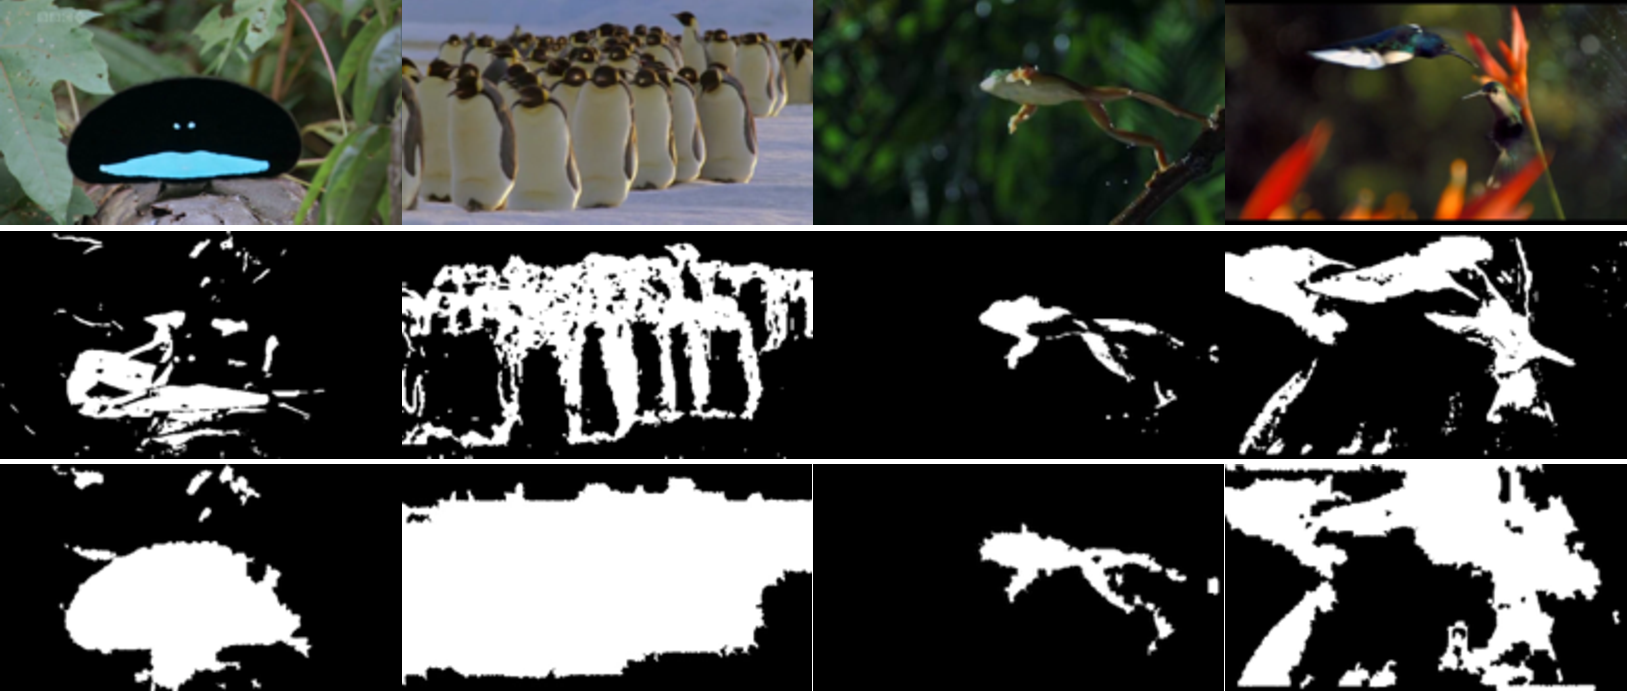
\includegraphics[width=0.97\textwidth]{figures/bs_vs_mask.pdf}
	\caption{Background subtraction masks vs. final masks. The first row demonstrates the original frames, the second row shows the masks generated by background subtraction methods, while the third row is the final masks produced by our method.} 
	\label{fig-bs-vs-mask}
\end{figure*}

We explored the effects of color spaces and different values of $\sigma$ in Equation~\ref{equ-rbf}. We perform the tests on the frog video.
% from SegTrack v2 dataset~\cite{f-li2013}. 
Figure~\ref{fig:sigma} shows the results of three color spaces and different values of $\sigma$. The advantage of one color space over others is not obvious. However, the values of $\sigma$ have an impact on mask quality, reaching a peak at a specific value indicating the appropriate amount of smoothing. In other experiments of this paper, we use the RGB color space and set $\sigma$ to $0.006$.

\begin{figure}
	\centering
	\subfigure[]{\label{fig:sigma} 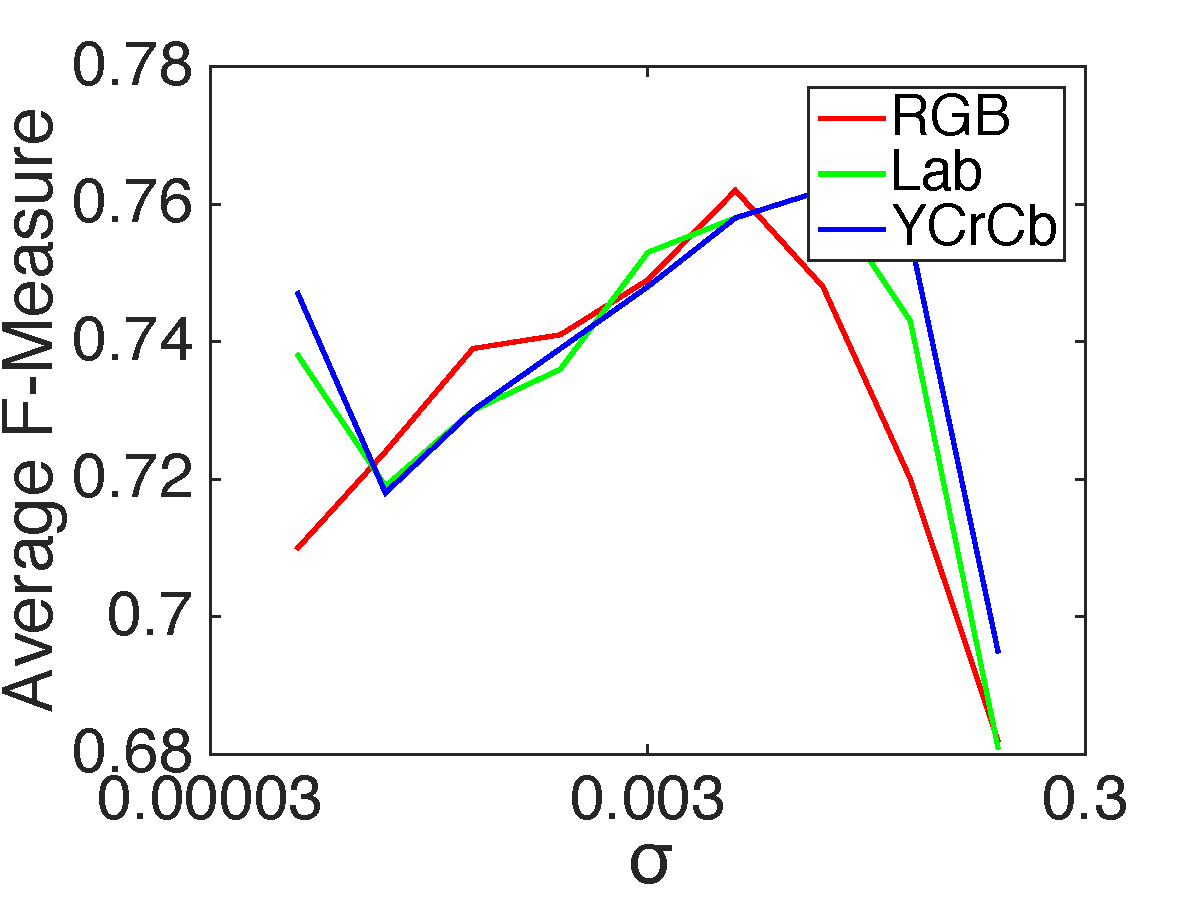
\includegraphics[width=1.65in]{figures/color-space-sigma.pdf}}
	\subfigure[]{\label{fig:constraints} 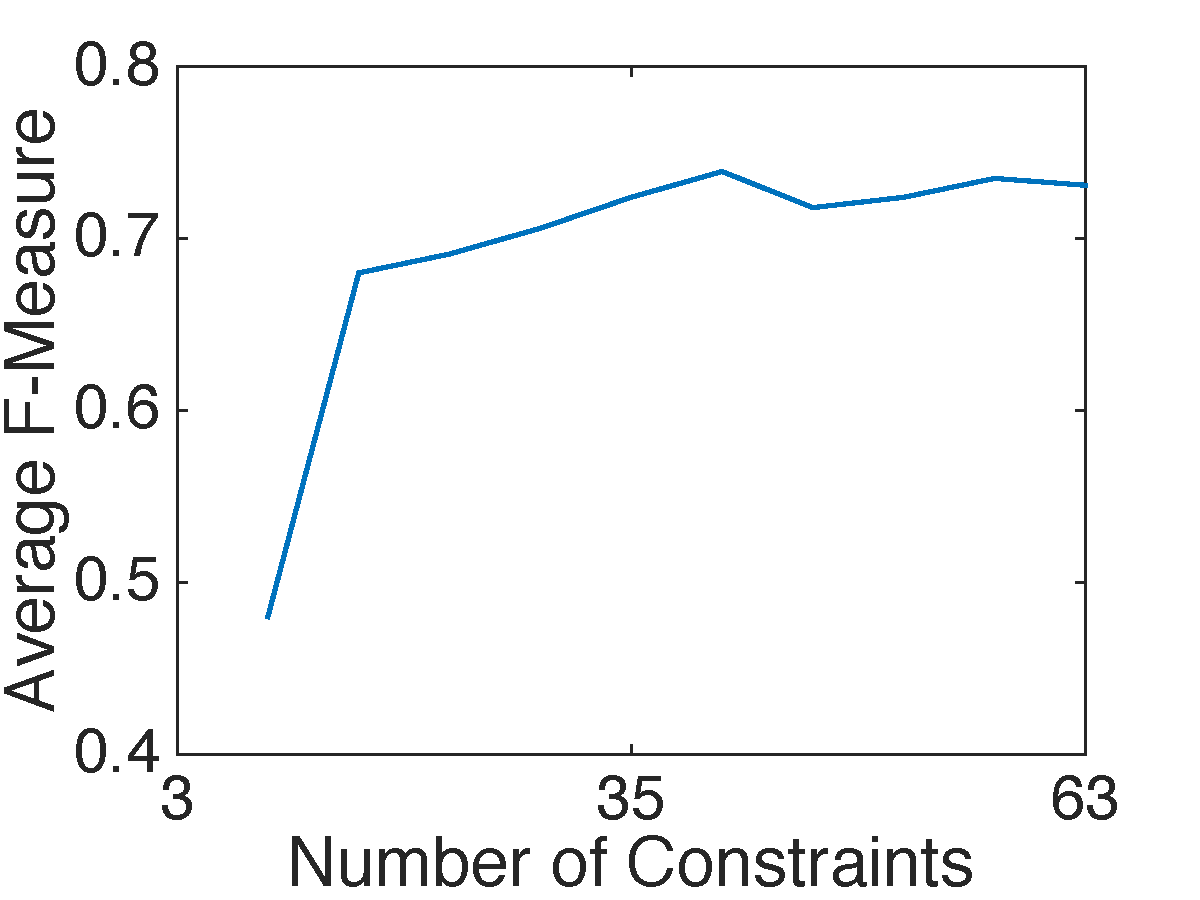
\includegraphics[width=1.65in]{figures/number_of_constraints.pdf}}
	\caption{Parameter Influence:~\ref{fig:sigma} $\sigma$ vs. F-Measure in color spaces RGB, Lab and YCrCb. ~\ref{fig:constraints} Effect of the number of constraints on mask quality. We evaluated the quality of the produced masks using the average F-Measure of the frames with different values of $\sigma$ and number of constraints.} 
%Other parameters are the same for all experiments. Three color spaces are examined, i.e. RGB, Lab and YCrCb, shown as red, green and blue, respectively.}
	\label{fig-params}
\end{figure}

When constructing the RBF, one important parameter is the number of constraints, i.e. the number of terms in Equation~\ref{equ-rbf-ef}.
%, which is used to solve the coefficients in \ref{equ-rbf}. 
As shown in Figure~\ref{fig:constraints}, the number of constraints impacts the mask quality. In this experiment, we set the number of Gaussians to 7, i.e. $|B|=7$. The number of constraints, i.e. $|E|$, is shown along the X-axis in
Figure~\ref{fig:constraints}.
% When $|E|=3$, it is even less than the number of Gaussians, thus the RBF is poorly solved. 
From $|E|=7$ to $|E|=35$, the quality of masks increases with the number of constraints. If we continue to increase $|E|$, there is no obvious benefit. Usually, we set $|E|$ as 2 to 5 times larger than $|B|$.

\section{Content-Aware Video Compression}
\label{sec:vos:cavc}

Video compression standards such as H.264/AVC compress videos as a whole. We applied the approach described above to conduct content-aware compression. We first extract the moving objects and blur the background using a bilateral filter. In this way, we obtain frames with original objects and blurred background. Then we use the obtained video as the input to a H.264 encoder. This method is effective in reducing the bitrate of compressed videos with the same encoding parameters since the blurred background has reduced high frequency components.
% than natual images~\cite{zhu2008}. 
The proposed content-aware compression shares some ideas with the block-based layered approach by Wang et al.~\cite{wang2012} and the sparsity decompression of Chen et al.~\cite{Chen2015}. Our approach is also related to seam carving for compression as proposed by Decombas et al.~\cite{decombas2012}.

\begin{figure*}
	\centering
	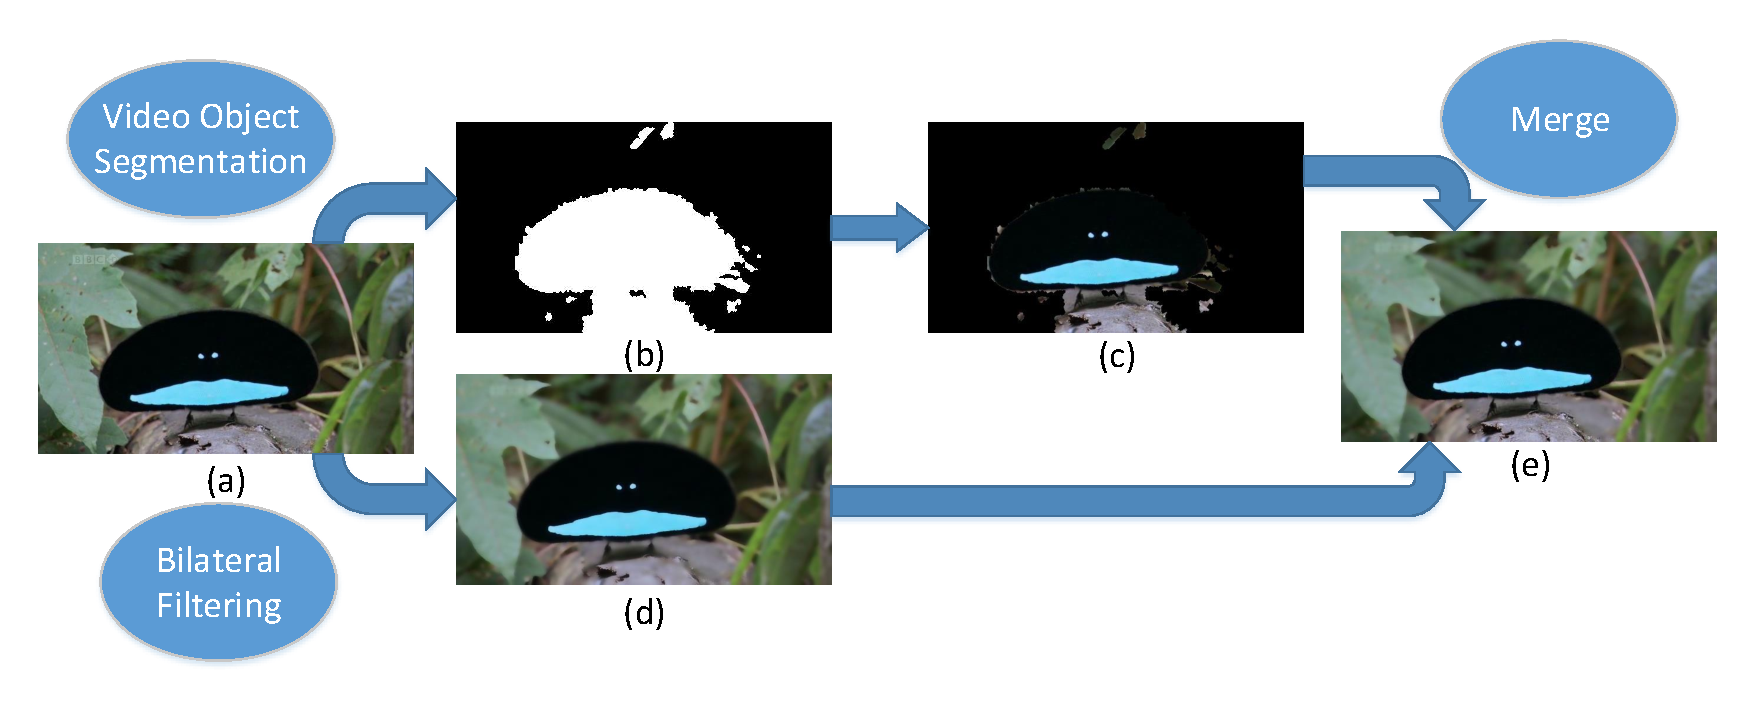
\includegraphics[width=0.97\textwidth]{figures/compression_workflow.pdf}
	\caption{Content-Aware Video Compression. (a) Original frame. (b) Mask generated with the video object segmentation method described above. (c) The object pixels covered by the mask. (d) The frame blurred with bilateral filter. (e) The merged frame.} 
	\label{fig-comp-wf}
\end{figure*}

Figure~\ref{fig-comp-wf} demonstrates the workflow of content-aware video compression. First, a mask (b) of foreground objects is generated with our video object segmentation method, followed by extraction of foreground pixels (c) covered by the mask. The original frame (a) is also blurred with the bilateral filter (d). Finally, the blurred image and the foreground regions are merged together (e). The composite frames are used as the inputs of a typical video encoder such as H.264/AVC. Our results demonstrate that this method can reduce the bitrate of compressed videos.

\begin{figure}
	\centering
	\subfigure[Inter-coding]{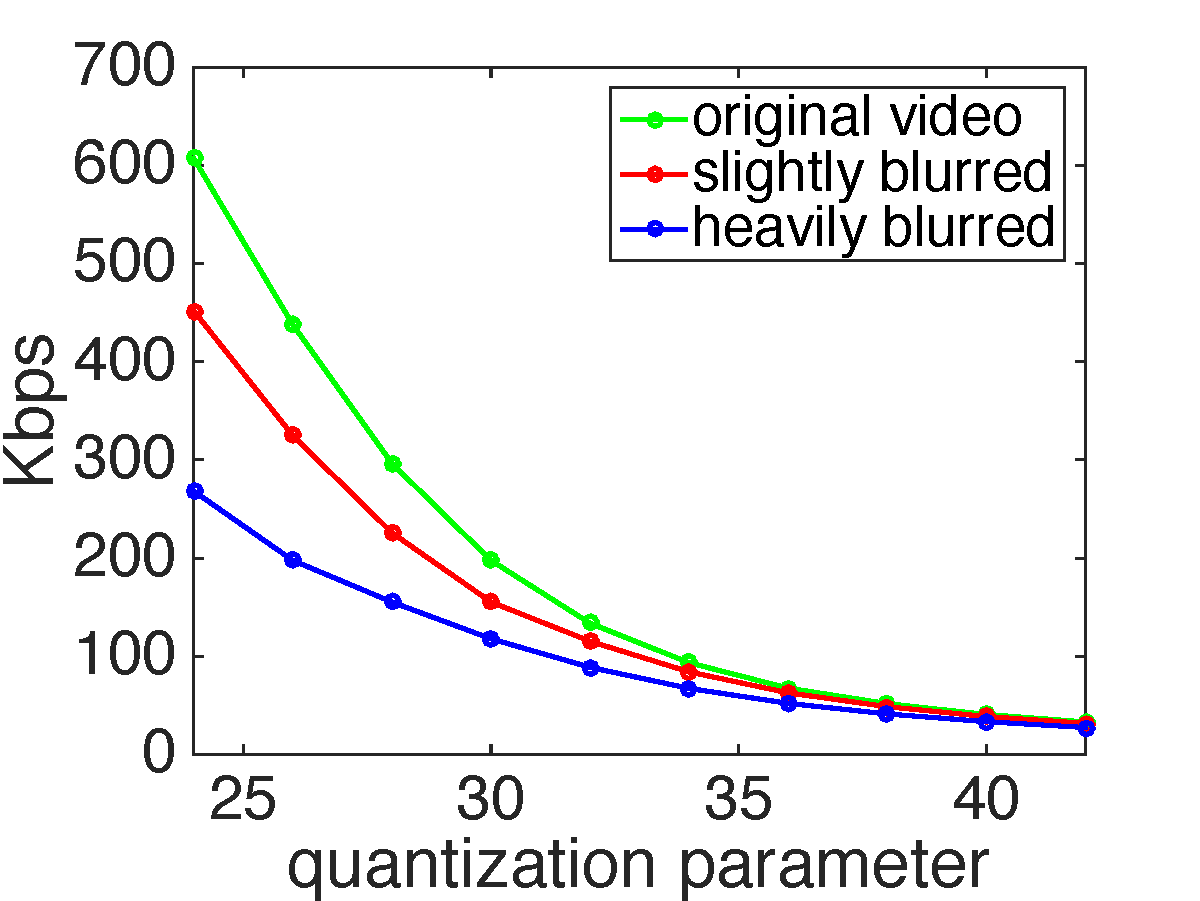
\includegraphics[width=1.65in]{figures/inter.pdf}}
	\subfigure[Intra-coding]{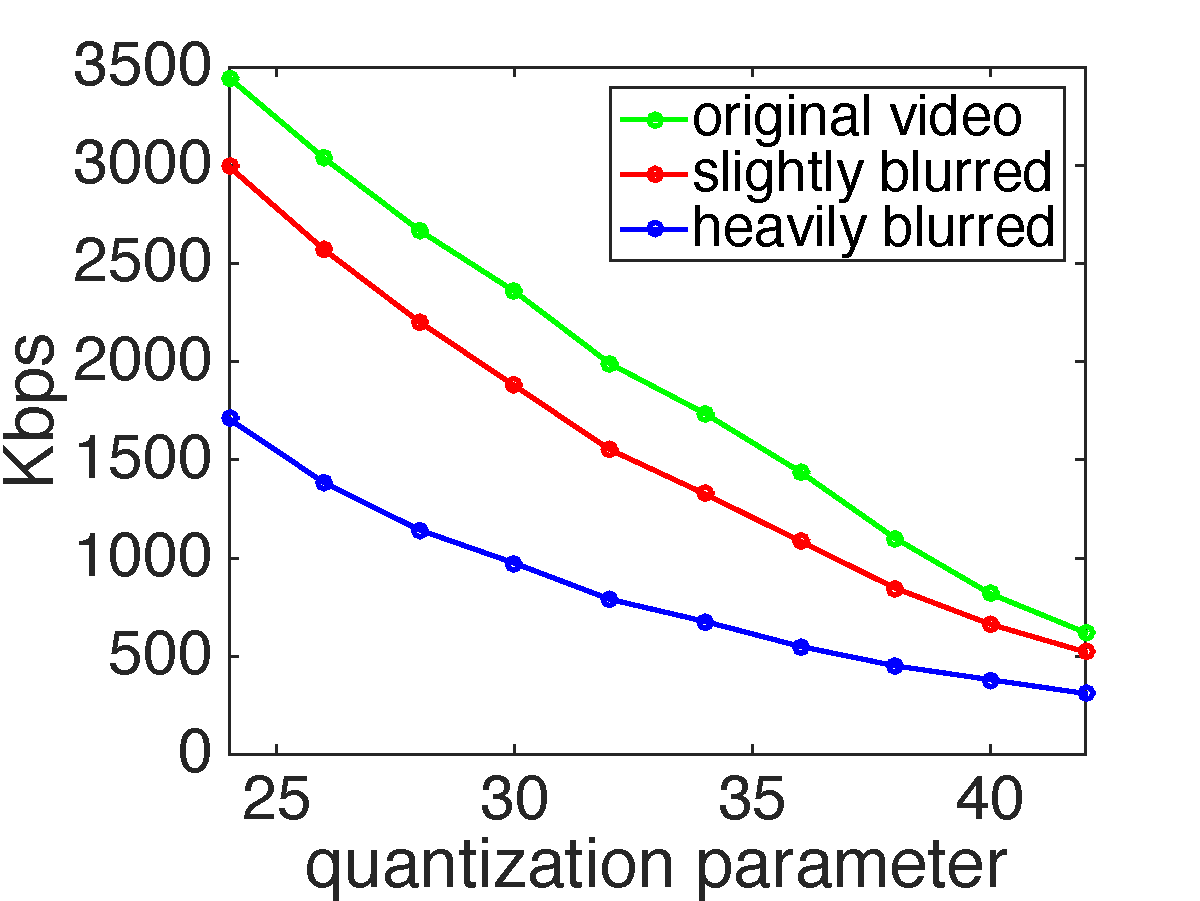
\includegraphics[width=1.65in]{figures/intra.pdf}}
	\caption{Bitrate of Compressed Videos. The X-axis shows the various quantization parameters, while the Y-axis is the bitrate (Kbps) of the compressed videos. The green lines are the bitrate of the original video, the red lines show the bitrate of the composite videos with slight blurring, and the blue lines demonstrate the bitrate of the composition videos but with heavy blurring. (a) and (b) show the results with different coding methods.} 
	\label{fig-comp-br}
\end{figure}

Figure~\ref{fig-comp-br} shows the effectiveness of our video compression method. Figure~\ref{fig-comp-br}(a) shows the results with H.264 inter-coding, while Figure~\ref{fig-comp-br}(b) demonstrates the results with H.264 intra-coding. The green lines illustrate the bitrate of the original video compressed by H.264, which has the highest bitrate among all three types of videos. The red lines show the composite video blurred with the bilateral filter and smoothing parameter set to $0.1$. The composite video achieves a lower bitrate than the original video. Moreover, with lower H.264 quantization parameters, the effectiveness of bitrate reduction becomes more noticeable. We also noticed that the bitrate reduction is higher with inter-coding than intra-coding, since background blurring benefits not only intra-frame compression, but also the prediction between frames. We also tried to increase the smoothing parameter of the bilateral filter, which gives a heavier blurring effect. The blue lines demonstrate the bitrate of the heavily blurred videos. For the inter-coding, the bitrate is slightly reduced, while for the intra-coding, the bitrate reduction is more obvious. We conclude that compression of videos with high-resolution foreground and blurred background can effectively reduce the bitrate, the quantity of reduction depends on the blurring degree of background, and the effectiveness is more noticeable with inter-coding than intra-coding.

%======================================================================
\chapter{Hybrid Remote Rendering}
\label{chap:hrr}
%======================================================================

% This part is the abstract of the paper with a minor change.
In this section, we present a hybrid remote rendering framework for applications on mobile devices. In our remote rendering approach, we adopt a client-server model, where the server is responsible for rendering high-fidelity models, encoding the rendering results and sending them to the client, while the client renders low-fidelity models and overlays the high-fidelity frames received from the server on its rendering results. With this configuration, the client is able to keep functioning regardless of network condition and bandwidth. Moreover, to minimize the bandwidth requirements, only key models are rendered in high-fidelity mode. We conduct a user study on factors that may impact the objective and subjective difficulty of an interactive task in a 3D mobile application. The results show that model fidelity has a significant influence on the objective difficulty, while network delay plays an important role in the subjective difficulty. The results of the user study explain how our method is able to benefit the users.

\section{Introduction}
\label{sec:hrr:i}

Mobile applications for gaming, training, healthcare among others rely on the rapid evolution of mobile devices in terms of both hardware and software.
Mobile devices offer a more intuitive interaction experience through gestures 
compared to PCs that mostly use traditional keyboard and mouse interfaces.
However, complex 3D models demand high-end computing hardware. Compared to PCs, mobile devices have much lower processing power, limited storage and less capable rendering hardware, even in most recent high-end mobile devices.
Developing mobile applications, especially 3D graphics applications, often requires simplification of the 3D models, leading to a degraded rendering quality.
Computationally intensive 3D graphics rendering tasks further burden the onboard battery.

One way to address the resource limitations of mobile devices is through Cloud Mobile Rendering (CMR).
CMR offloads computationally intensive rendering to cloud servers:
the server initializes a rendering engine and an encoder to serve every connected client. The models are rendered on the server side and encoded in video frames streamed from the server to the client~\cite{lamberti2007,lu2011,ma2017,chang2004,simoens2012}.

However, CMR systems often require a very high network bandwidth, which is seldom available and suffers from interaction latency~\cite{chen2014}. Various attempts have been made to improve such systems. 
Boukerche and Pazzi~\cite{boukerche2006} use environment maps rendered on a server and sent to the client to reduce bandwidth. The client is able to respond to user interactions, resulting in panning and tilting without latency based on the environment map.
Shi et al.~\cite{shi2012} propose a framework that leverages depth maps to reduce interaction latency. They take advantage of 3D image warping to synthesize the mobile display from the depth images generated on the server.
However, theses two image-based rendering techniques assume static scenes and only support limited user interactions.
For example, the use of environment maps by Boukerche and Pazzi~\cite{boukerche2006} accelerates panning interactions, but a new environment map needs to be generated for a novel viewpoint, which increases interaction delay and bandwidth requirements. Similarly, at scene changes, the environment maps or the depth maps also need to be regenerated in the approach proposed by Shi et al.~\cite{shi2012}.

We propose a remote rendering system that minimizes the network bandwidth requirements in remote rendering.
Our approach is a client-server architecture and maintains two versions of models: low-fidelity models and high-fidelity models.
Low and high fidelity models differ in the number of polygons and in rendering quality.

On the client side, the mobile device renders low-fidelity models that have less polygons, lower fidelity of textures, and lower quality rendering effects, while on the server side, the workstation renders high-fidelity models that have more polygons, higher fidelity of textures, and higher quality rendering effects. Hence, key models are rendered on the server and captured in images that are sent to the client as a video stream. We define key models as those that the user is interacting with. These models can be identified from interaction information sent to the server. Additional key models may be specified in advance by the developers based on application-specific criteria.

The proposed architecture is able to reduce the required network bandwidth and latency in user interactions.
Since only the regions of interest of the entire frame are encoded and streamed to the clients while the rest is discarded, it reduces the bit rate of the encoded video stream.
The user interaction latency is composed of three components: rendering, encoding, and network transmission. Our proposed method aims at reducing the rendering and encoding time by only rendering and encoding the key models in high-fidelity mode and rendering the rest in low-fidelity mode without encoding.
Because the frames are encoded and streamed over non-dedicated networks, of which the conditions often do not satisfy the requirements of remote rendering applications. The most important contribution of the proposed framework is enabling a trade-off between rendering quality and network delay, which is essential but existing remote rendering applications cannot address this issue.

\section{Background}
\label{sec:hrr:bg}

Games, training, medicine, and many other applications in everyday life~\cite{ramanathan2007,chun2011,kwon2017,rodriguez-gil2017} leverage the advantages of mobile devices with their rapidly progressing hardware and software.
The touch-based interaction on mobile devices is arguably more intuitive than the use of keyboard and mice on PCs. Nevertheless, mobile devices have their limitations when it comes to rendering and interacting with complex 3D models, e.g. lower processing power, limited storage, and less capable rendering hardware.
Computationally intensive 3D graphics rendering tasks also impose severe challenges on the limited battery capacity of mobile devices.

To address these issues, remote rendering can be employed. This technique leverages the computational capacity of a remote server to relieve the rendering burden on the client side.
One direction in this field is partitioning and simplifying large and complex 3D meshes on a server and sending a part of simplified meshes to the client. Park and Lee~\cite{park2016} propose a framework to enable users to view large meshes on mobile devices hierarchically. Depending on various scales, meshes with different Level Of Detail (LOD) are generated on the server and transmitted to the clients.
However, transmission of meshes with different LOD frequently increases power consumption. Yan et al.~\cite{yan2014} propose the algorithm ASEHM that minimizes the transmission frequency in sending 3D meshes. Instead of transmitting a new level of the same model, ASEHM refines a coarser LOD into a higher-fidelity LOD, provided that the relationship between the LODs is available.

Another research direction is offloading the entire rendering task to the server. Basically, when a mobile client connects to the server, the server will initialize a rendering engine and an encoder for the mobile client. All the models are rendered on the server side and rendered frames are encoded and streamed from the server to the client as a video stream. Moreover, the server receives user interaction feedback from the client. This approach requires no 3D graphics capacity on the client and is able to use advanced encoding, such as H.264/AVC, to adjust the image quality according to the bandwidth availability.
Lamberti and Sanna~\cite{lamberti2007}, Moimark and Cohen-Or~\cite{noimark2003}, and Lu et al.~\cite{lu2011} have proposed such CMR systems.
Many cloud gaming services and frameworks have leveraged this technology, such as OnLive\footnote{http://onlive.com}, NVIDIA GeForce Now\footnote{https://www.nvidia.com/en-us/geforce/products/geforce-now/}, PlayStation Now\footnote{https://www.playstation.com/en-ca/explore/playstationnow/} and Gaming Anywhere\footnote{http://gaminganywhere.org}. Those services and frameworks use the cloud computing infrastructures to render the games and encode the rendered frames, while the clients decode the rendered frames and send the players' interactions to the cloud.
The primary disadvantage of this type of approach is the introduction of additional latency, including user interaction transmission time, rendering and encoding time at the server side, image transmission time, and decoding time at the client side~\cite{shi2015}. However, minimizing the latency is challenging considering the high uncertainty of the network transmission. Using a geographically proximate server helps to greatly reduce the latency since every 1000 miles of physical distance adds 25ms round-trip delay to the overall latency~\cite{perlman2010}.

To relieve the heavy dependence of remote rendering methods on the network, researchers proposed various methods~\cite{paravati2010,liang2009,yang2013}. One type of those methods uses environment maps to accelerate rendering, e.g., 
Boukerche and Pazzi~\cite{boukerche2006} render environment maps on the server and send them to the client. With the environment map, the client is able to respond to the user interaction in the form of panning, tilting and zooming without latency. Environment maps have some similarity to panoramas that were originally proposed by Chen~\cite{chen1995} in their QuickTime VR system, which displayed virtual environments without rendering 3D models.
QuickTime VR accomplished moving through the environment by "hopping" to different panoramic points.
Boukerche and Pazzi~\cite{boukerche2006} do not simulate movement by "hopping" to another panoramic image; instead, they use a remote server to render panoramic images in real-time. They address the delay in rendering and transmitting panoramic images through a caching design that buffers visited viewpoints.
A common disadvantage of methods that use environment maps is that they only handle static environments, and navigation typically leads to wait times for the user. If the objects in the scene move or the user navigates, re-rendering and re-transmission of environment maps can lead to latency~\cite{macchiavello2014,quax2016}.

Some researchers attempted to leverage the advantages of a depth map to synthesize new views on the client. 
Shi et al.~\cite{shi2012} proposed a framework that leverages depth maps to reduce user interaction latency. They take advantage of 3D image warping to synthesize the mobile display from the depth images generated on the server.
Chang and Ger~\cite{chang2002} proposed building Layered Depth Images (LDIs) on the server. The mobile device uses a 3D warping algorithm to synthesize the frame from a new view point.
At the time of the design of LDIs, mobile devices had almost no capacity to render 3D scenes and hence LDIs were designed as a way around displaying 3D content on a mobile device. 
These image-based methods incorporating scene depth often face issues with visible gaps and holes in the rendered scene. Bao and Gourlay~\cite{bao2006-1,bao2006-2} proposed a method that uses a superview to direct the image warping and reduce the gaps and holes.
The method is successful in reducing the flaws in the synthetic images. However it is not designed to handle highly dynamic scenes, since a set of new reference depth maps need to be generated and delivered to the client whenever the scene changes. Their method is well suited for environment walkthrough applications but not for games and training applications.

Other approaches support dynamic scenes and all types of interactions. They accelerate the data transmission to adapt to various network environments or reduce interaction delay.
Levoy~\cite{levoy1995} proposed a method that renders simplified models on clients to reduce bandwidth requirement. In this method, the server first renders both complete and simplified models and calculates a difference image between the two. Then the simplified model and the difference image are transmitted to the client. Finally, the client renders the simplified models and applies the difference image to produce a high-quality rendering. The simplification of models can be performed in terms of the textures and the number of polygons. This method reduces the bandwidth requirement for obtaining a high-quality rendering. Compared with our method, this work shares the same idea of using simplified models. However the difference is that Levoy~\cite{levoy1995} uses simplified models to achieve a compression effect on image transmission, while our method uses simplified models on the client side for display and interaction. Also, our simplification is selective and achieves a bandwidth reduction by rendering environment models only on the client.
Liu et al.~\cite{liu2014} extended image streaming and developed an automatic adaption algorithm that changes the rendering quality according to the network bandwidth. They use H.264 video encoding with fixed bit rate mode while adapting the rendering factors (e.g. view distance, realistic effect and texture detail) to improve the user experience. The goal of this method is to improve the visual quality of encoded frames with insufficient network bandwidth.
However, the rendering quality of all models is adapted at the same level since H.264 video encoding does not distinguish the importance of key models and environment models in a scene. Their work also does not address one of the most severe issues in remote rendering, interaction latency.
Hemmati et al.~\cite{hemmati2013bitrate} proposed a method for cloud gaming, which selectively renders important objects and reduces video bitrate by not rendering unimportant objects. However, they did not answer the question about how it influences user experience.
Inspired by Hemmati et al.~\cite{hemmati2013bitrate}, Lu et al.~\cite{lu2017selective} proposed an approach that maximizes user experience with limited network bandwidth for stereo video streaming. In this approach, the left view and right view are rendered asymmetrically in terms of texture detail, and certain objects are not rendered in on view. This technique enables intelligent decision of whether or not to render an individual object and how good the corresponding texture detail will be if rendered.

We propose a general-purpose remote rendering framework. By only rendering key models remotely, our method minimizes the network bandwidth requirement.
It enables a trade-off between rendering quality and network delay.
We do not assume a priori knowledge about the application, and thus, our framework is able to handle dynamic scenes and all types of interaction (e.g. motion, panning and zooming). We also benefit from the increasing rendering capabilities of mobile devices while addressing the fact that mobile devices still fall behind PCs. We believe that the idea of offloading the entire rendering task to the server may be outdated given the recent advances in mobile device hardware.

\section{Method}
\label{sec:hrr:m}

\subsection{Client-Server Prototype Design}
\label{sec:hrr:m:cspd}

Our proposed system aims at providing high-quality rendering on less powerful mobile devices, while minimizing the amount of data transferred via the network. We would also like to enable multi-client cooperation to enhance the user experience in training scenarios.

Our system is inspired by Levoy~\cite{levoy1995}, Lamberti and Sanna~\cite{lamberti2007}, and Lu et al.~\cite{lu2011}. It uses a hybrid approach incorporating both local and remote rendering.
Hence, the low-fidelity key models are stored on the client-side and the local rendering capacity is leveraged to produce lower quality rendering results.
Conversely, the high-fidelity renderings of key models are sent from the server to the client and overlaid upon the locally rendered frames.
Accordingly, the data transferred via the network is minimized due to the small amount of pixels that are sent via the network compared to a CMR solution. 

There are three challenges in realizing multi-client support within the context of the above-described system.
First, it is required that the server must not be blocked by any of the clients.
Second, each client has its own view that may be different from all the other clients; and this can result in a performance issue as a scene needs to be rendered multiple times in a single animation loop.
Third, because only key models are rendered and sent by the server, occlusion becomes a problem since the environment models that are closer to the viewpoint may not be rendered on the server but just locally.

We address the first problem by mandating that the server interacts with each client independently. More specifically, we enable the server to receive commands from and send to every client separately, so that if a client becomes unresponsive, the server is not blocked.
The second issue is alleviated by implementing a "render-on-demand" function on the server, which means that the server renders the scene for a client only when the client requires a new frame.
We address the third challenge through a two-pass rendering process. In the first pass, the entire scene is rendered in low fidelity on the server. Then the colour buffer is cleared before the second pass, where only the key models are rendered in high fidelity. In this way, the second pass is rendered with the depth information obtained from the first pass.

\begin{figure}[!htbp]
	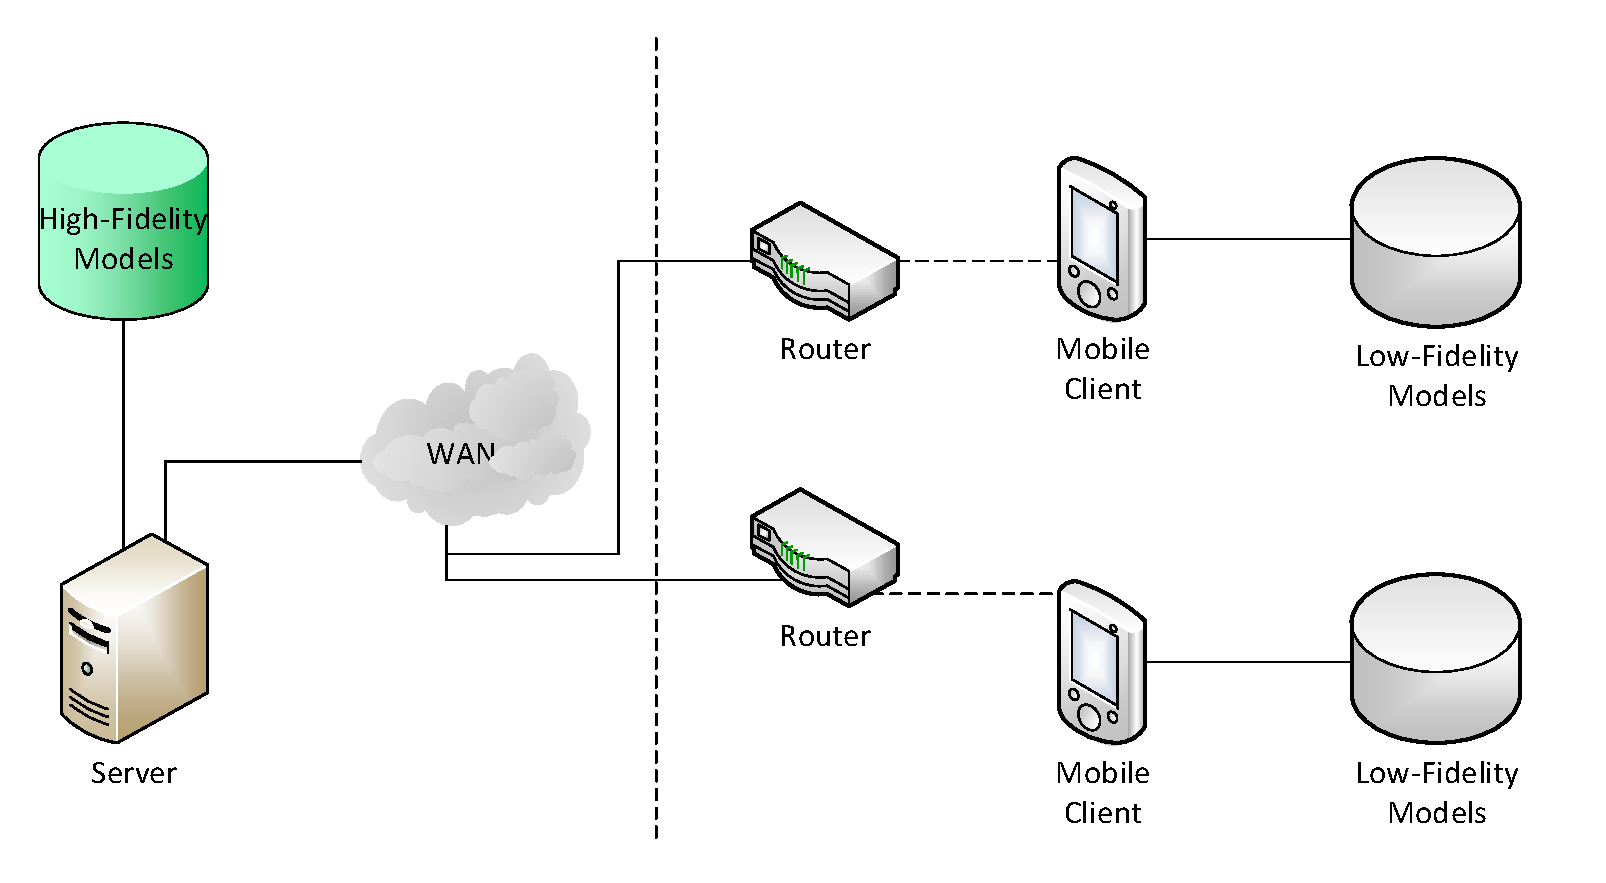
\includegraphics[width=\textwidth]{figures/architecture.pdf}
	\caption{System architecture}
	\label{fig:architecture}
\end{figure}

\begin{figure}[!htbp]
	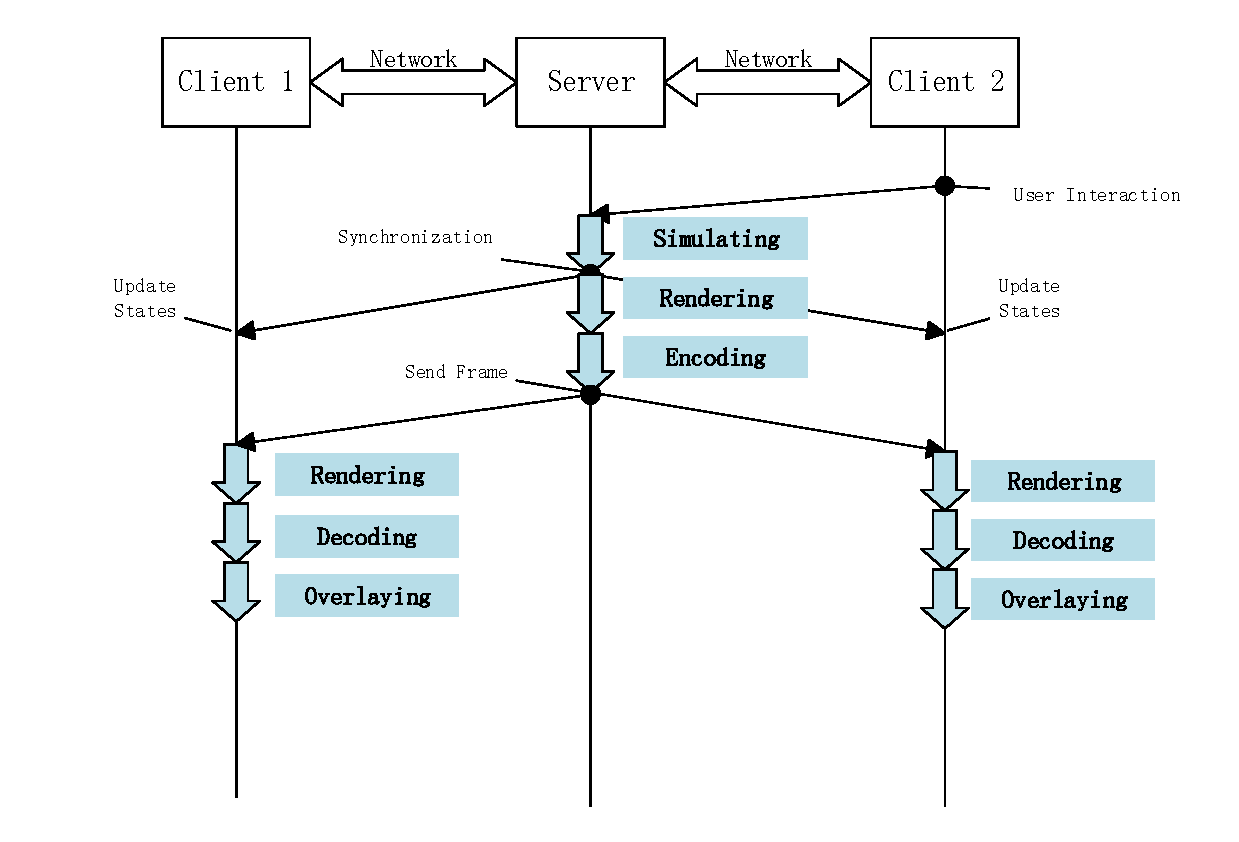
\includegraphics[width=\textwidth]{figures/sequence_workflow.pdf}
	\caption{Workflow of communication between the server and the clients}
	\label{fig:swf}
\end{figure}

As depicted in Figure~\ref{fig:architecture}, in this system, all clients are connected to the rendering server and send interaction commands to the server.
On the server side, the application status changes according to the commands received from all clients. The application status changes are synchronized with all clients. In this way, the clients are able to cooperate with each other. In other words, when a client changes the status of the application, all clients will see the change after synchronization.
To minimize the amount of transferred data, the client decides which models need to be rendered in high-fidelity and the server only sends the pixels depicting those key models. The other models are still rendered locally.

Figure~\ref{fig:swf} illustrates the sequence of messages communicated between the server and the client processes. It shows the tasks that are performed by the server and clients to process one frame. If the commands sent from any client influence the simulation states of the server, the latter synchronizes the state changes among all clients to ensure that all of them maintain a consistent state. Moreover, the server renders and encodes the frames for all the clients. Upon receiving the high-fidelity frame, the client decodes and overlays it on the locally rendered frame.

\subsection{Process Behavior}
\label{sec:hrr:m:pb}

The proposed system consists of one server and multiple clients.
Figure~\ref{fig:s-wf} shows the behavior of the server process.
In each loop, the server updates the simulation status of the scene and receives commands from all clients.
Next, the server sends the received commands to all clients to ensure synchronization among them.
On the server side, each client has its own view that is independent from those of the other clients.
The server only renders a new frame upon request from the client.

Figure~\ref{fig:c-wf} shows the behavior of the client processes. In each loop, the client receives commands from the server and adjusts the simulation status accordingly. Then, it sends its user interaction commands to the server. In each iteration, the client will receive the high-fidelity frame from the server that it has requested in the previous iteration. The client has simplified models stored locally, which renders the scene in every iteration. The high-fidelity frames acquired from the server are overlaid upon the locally rendered frames. Once done, it sends the frame request to the server. In this way, the server does not need to render frames for all clients in every loop; instead, it renders a frame when it is needed.

\begin{figure}[!htbp]
	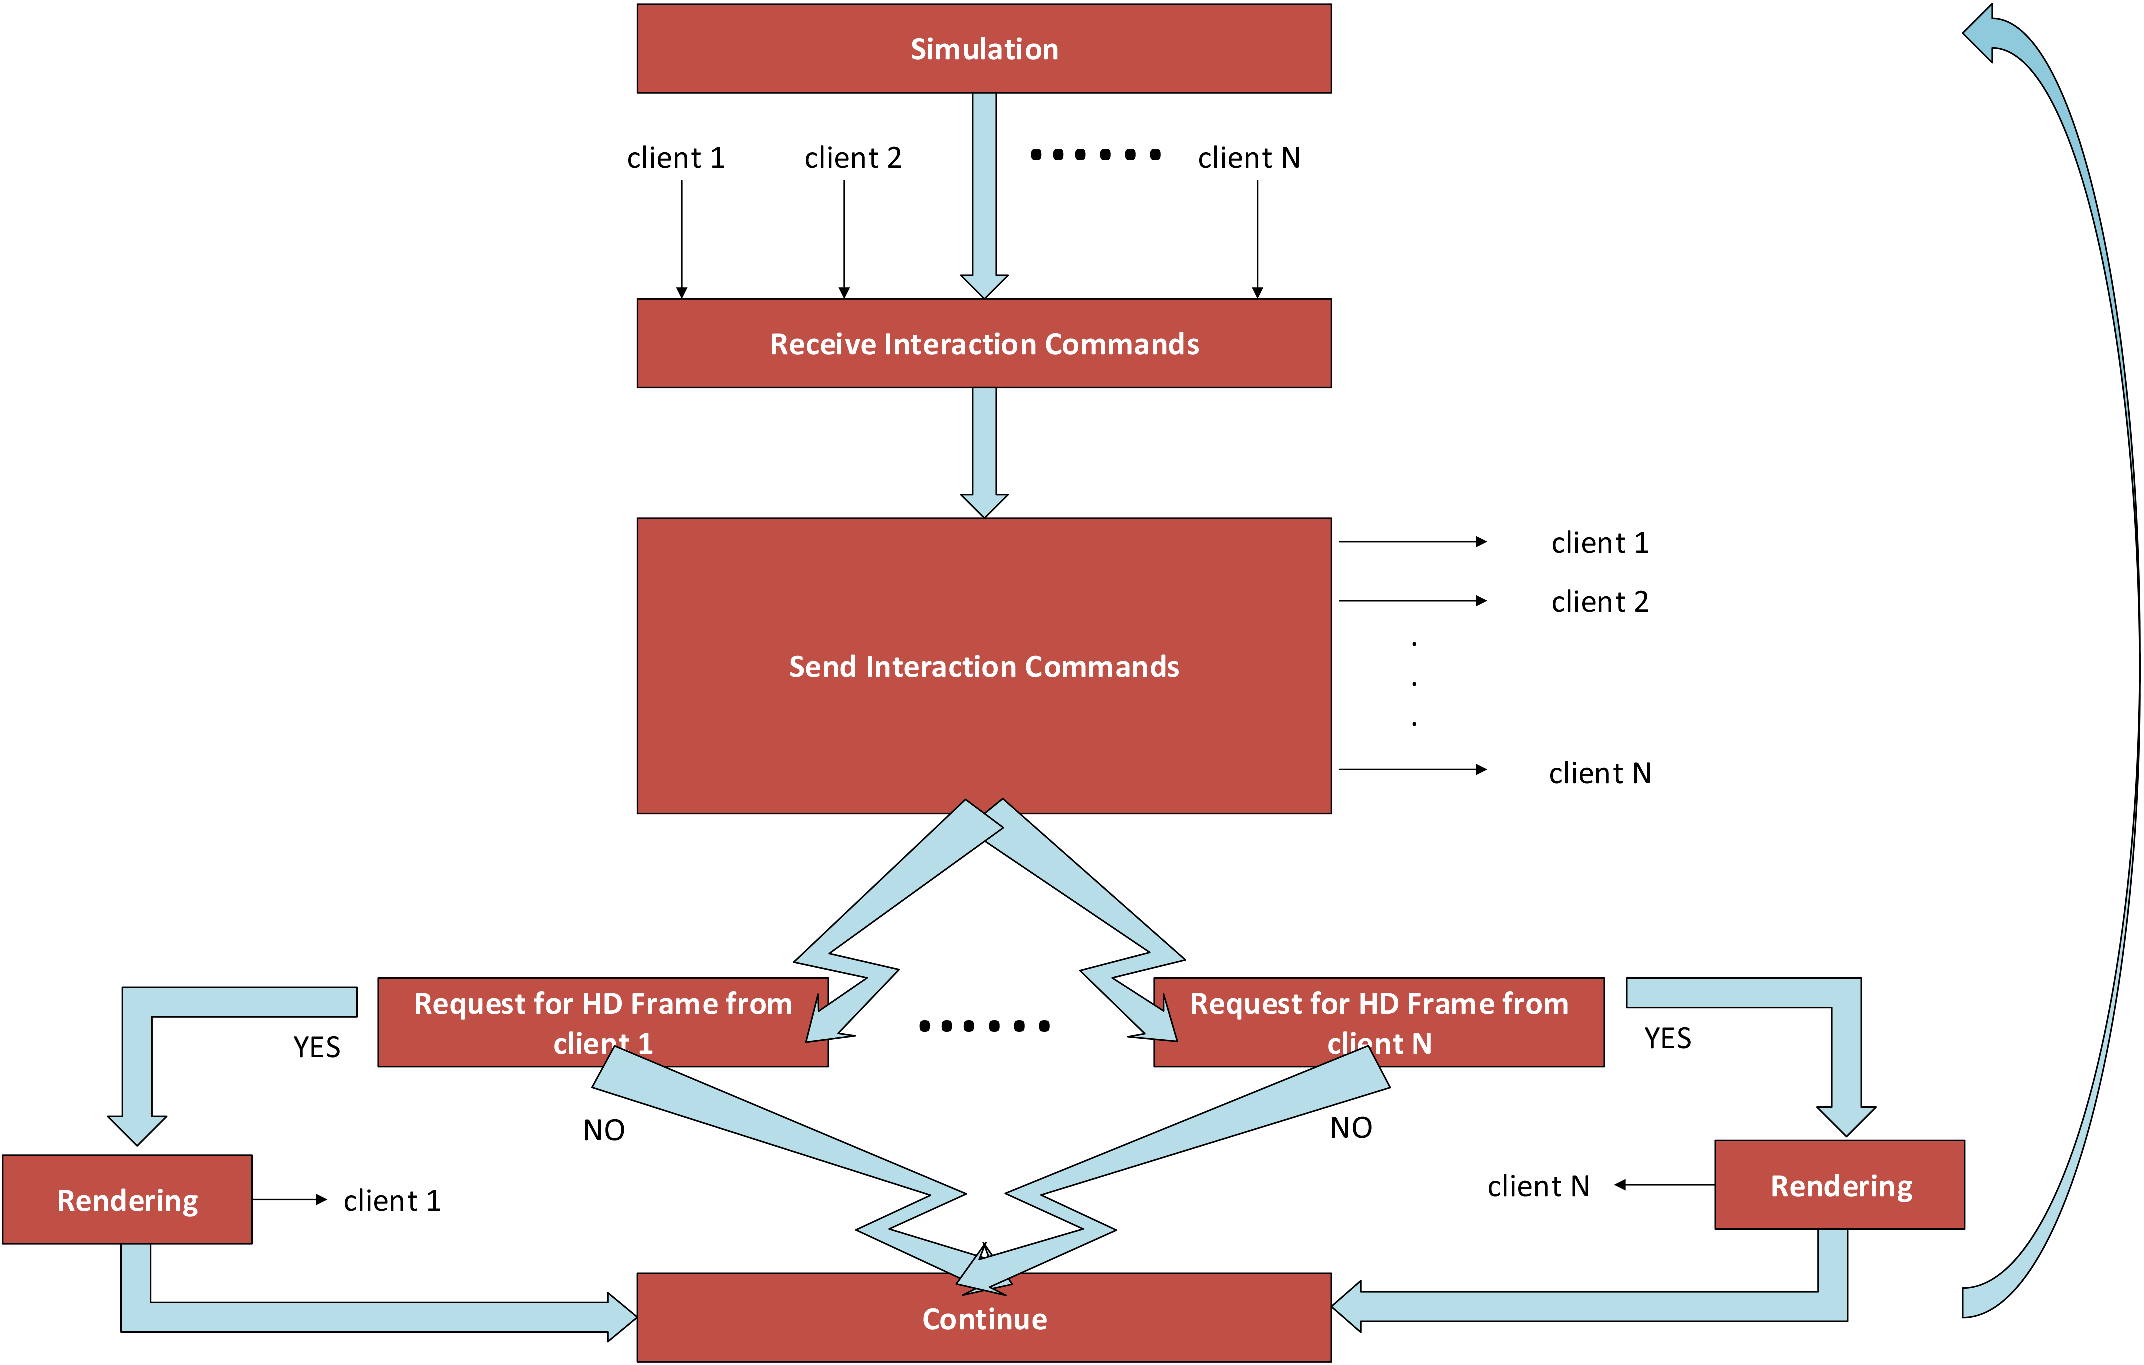
\includegraphics[width=\textwidth]{figures/workflow_server-eps-converted-to.pdf}
	\caption{Server-side Workflow}
	\label{fig:s-wf}
\end{figure}

\begin{figure}[!htbp]
	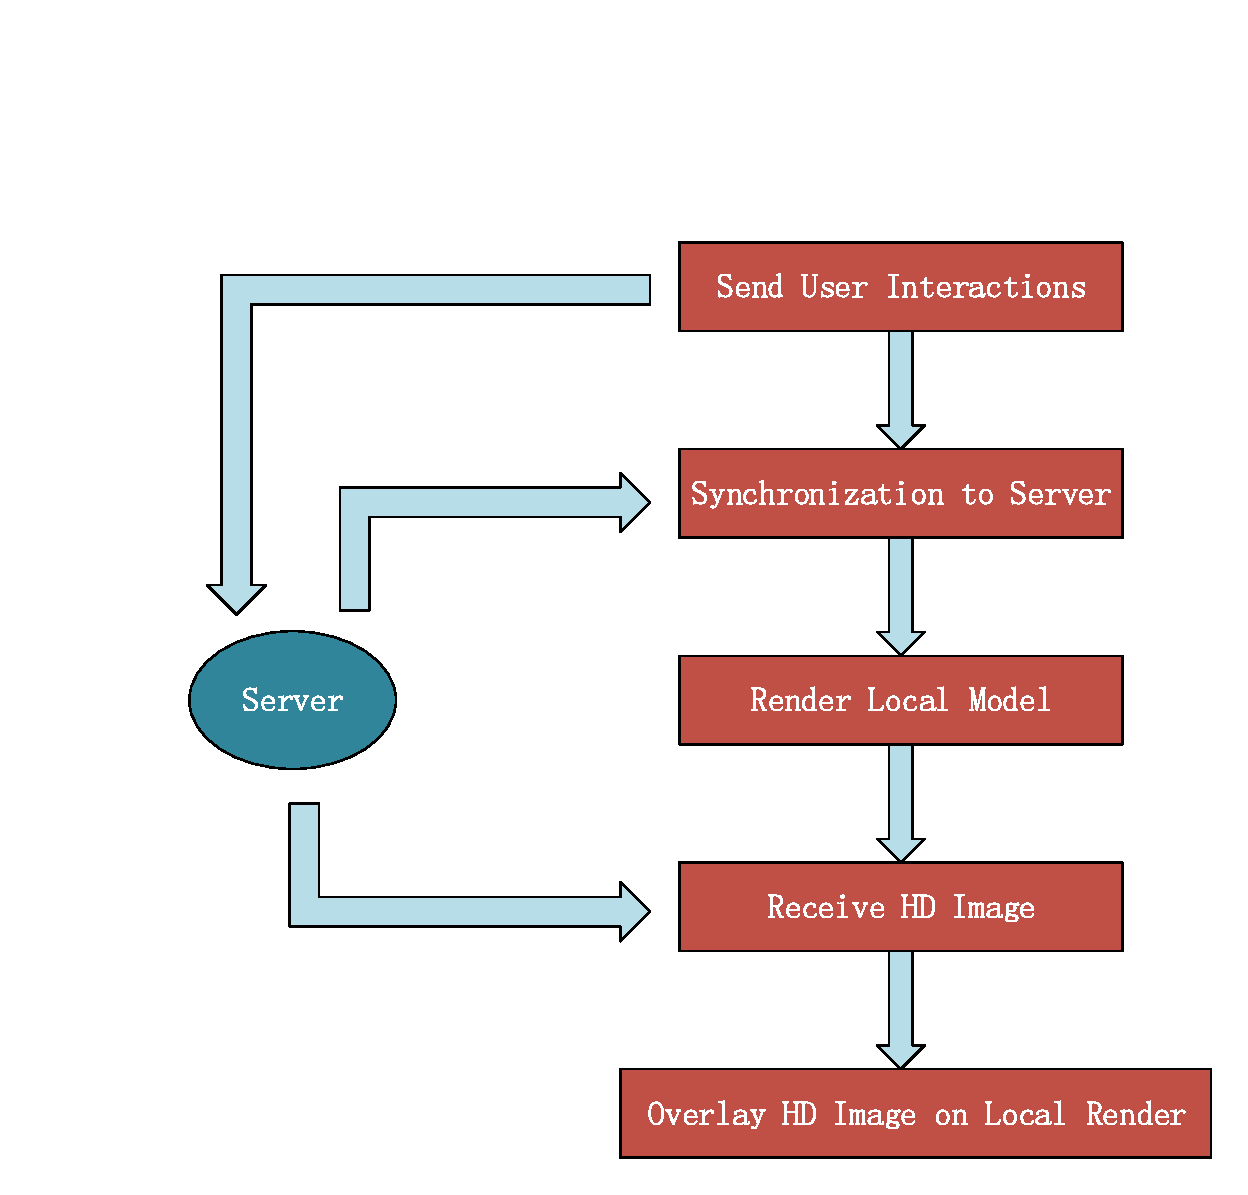
\includegraphics[width=\textwidth]{figures/workflow_client.pdf}
	\caption{Client-side Workflow}
	\label{fig:c-wf}
\end{figure}

\subsection{Two-pass Rendering}
\label{sec:hrr:m:tr}

As mentioned in Section~\ref{sec:hrr:m:cspd}, we use a two-pass rendering process on the server side.
The frames sent to the client depict only high-fidelity key models.
However this is not enough for valid view of the 3D scene since other scene content may occlude parts of the key models.
We propose a two-pass rendering process to address this issue.

\begin{figure}[!htbp]
	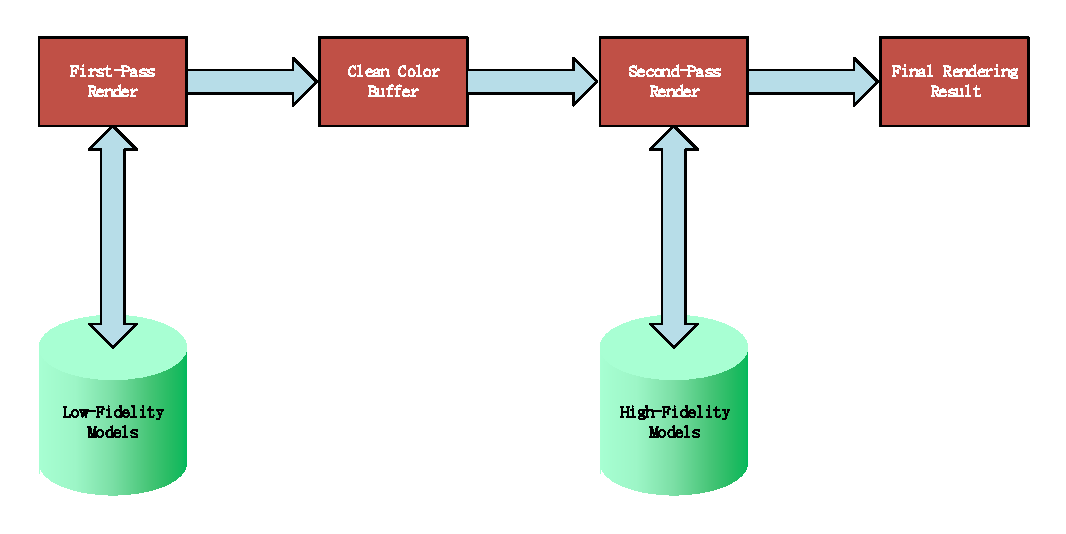
\includegraphics[width=\textwidth]{figures/two-pass-rendering.pdf}
	\caption{Two-pass rendering}
	\label{fig:tp-rendering}
\end{figure}

As shown in Figure~\ref{fig:tp-rendering}, in the first pass, all models are rendered in low-fidelity except for the key models. Then the color buffer is cleared, and only the depth buffer is preserved. In the second pass, only the high-fidelity key models are rendered, while considering the depth information obtained from the first pass rendering. Therefore, the occlusions are preserved in the final rendered scene.

\section{User Study}
\label{sec:hrr:us}

In Section~\ref{sec:hrr:m}, we propose a hybrid remote rendering framework that offloads a part of the rendering task to the remote server. More specifically, only key models are rendered remotely to minimize network bandwidth requirement and network delay.

To overcome the limitations of mobile devices in rendering high-fidelity models, designers often use one of the two approaches:
\begin{enumerate}
\item
Local-only rendering: Reduce the fidelity of the models and render them locally on mobile devices.
\item
Server-only rendering: Render the scene remotely on a server and transfer to the mobile phone client as a video stream.
\end{enumerate}

However, both approaches risk reducing the user's Quality of Experience (QoE). For the local-only rendering approach, the user is interacting with models that are not rendered at their optimal quality. Fine details in the model might be missing, which reduces the aesthetics of the scene. Also, for some applications, these details might carry important information. For instance, it is important for users in many gaming applications to quickly distinguish between similar objects in a scene. Objects rendered as low-fidelity models might not be immediately discernible. For the server-only approach, QoE might be affected by a long delay between the user's actions and application's response. This would be mostly caused by the network delay between client and server. Furthermore, bandwidth limitations can cause interruptions in the video stream.
The proposed approach strikes a balance between local-only rendering and server-only rendering. It renders only key models remotely at high-fidelity while other models are rendered locally at low-fidelity. 

Previous work has explored how various factors affect the user experience. Hong et al.~\cite{hong2015user-study} conducted a subjective user study to quantify the effect that video bitrate and frame rate have on QoE in cloud gaming.
Slivar et al.~\cite{slivar2015qoe} use Steam In-home streaming platform\footnote{http://store.steampowered.com/streaming/} as a case to study how the frame rate and bitrate influence the QoE. They model the QoE as a combination of two aspects: perceived graphics quality and perceived game fluidity.
In the work by Suznjevic et al.~\cite{suznjevic2016}, five factors (i.e. latency, jitter, packet loss, frame rate and frame resolution) are studied in terms of their effects on the QoE of NVIDIA GeForce Now platform.
Hemmati et al.~\cite{hemmati2013bitrate} developed an algorithm that minimizes bitrate by not rendering unimportant models. Our method leverages a similar idea by rendering key models in high fidelity and environment models in low fidelity. However, the difference is that our method renders the environment models locally instead of not rendering them at all.

Our method targets not only gaming, but also other types of applications, such as training applications and virtual tours. The expectations of users in terms of graphics quality and application fluidity may depend on the different types of applications. For instance, the players of a game may focus on the quality of special effects, while the users of a surgery application may focus on how clearly anatomical features can be distinguished. Thus, we do not measure QoE but how difficult it is to accomplish a given task. Thus, we are interested in the effects of the key model fidelity and environment fidelity on the perceived diffculty of task completion. We name this measure the Difficulty of Task (DoT). We measure DoT in two ways: Objective DoT (ODoT) and Subjective DoT (SDoT).
The ODoT is a measure of how well the users can accomplish a task. It might be measured by a score or a level calculated by the application.
The SDoT is a measure of the users' opinion on the task difficulty and can be answered by a subjective questionnaire.

Our user study was approved by the Research Ethics Board at the University of Ottawa (File Number: H12-16-05).
The main user study is informed by a pre-trial study discussed next.

\subsection{Pre-Trial Study}
\label{sec:hrr:us:pts}

A major goal of the main study is to analyze the effect of 3D model fidelity on the DoT. However, in the proposed framework, there are two types of models: high-fidelity models and low-fidelity models. Those models will be used in the main study (see Section~\ref{sec:hrr:us:ms}). We have prepared 15 high-fidelity models and simplified them to obtain low-fidelity models using QSlim~\cite{garland1997}.

\subsubsection{Objective}
\label{sec:hrr:us:pts:o}

The objective of the pre-trial study is to decide the number of polygons for the low-fidelity models. If it is too low, the participants will not be able to recognize the object that the model represents. In the pre-trial study, we want to find out at which point the object represented by the model becomes discernible to the majority or all subjects.

\subsubsection{Participants}
\label{sec:hrr:us:pts:par}

We recruited 5 participants, 4 males and 1 female. None of the subjects was visually impaired.

\subsubsection{Independent Variables and Dependent Measures}
\label{sec:hrr:us:pts:ivdm}

The experiment was conducted with one independent variable: number of polygons of the surface mesh in the 3D model.
The independent variable has 50 levels. For the first level, the model is composed of 20 polygons. For each of the 49 subsequent levels, the number of polygons is increased by $10\%$. We measure the number of polygons necessary for a subject to recognize the object for each 3D model.

\subsubsection{Procedure}
\label{sec:hrr:us:pts:pro}

The experiment was conducted using a program that shows 15 models at different levels of fidelity.  We created 50 levels of fidelity for each model by starting with 20 polygons and increasing its polygon count by $10\%$ for every level using QSlim~\cite{garland1997}. Our program showed the subjects a model on the screen and asked them to select the object it represents from a side menu by choosing among a dog, a cat, a horse, and unknown. Subjects were instructed to choose the unknown option if they were unsure. We started with a model with very low polygon count (20 polygons). Every time the subject selected an answer, we increased the polygon count to the next level adding more details to the model. The order through which the models were shown to the subjects was randomized to avoid biasing the results. 

\subsubsection{Results}
\label{sec:hrr:us:pts:r}

\begin{table}[!htbp]
\caption{Data collected from the pre-trial study, which represents the number of polygons above which a participant ceases to make mistakes. However, in one case, one of the participants does not recognize the model even at full resolution (marked by a dash). The numbers in bold are those selected as the final number of polygons of the low-fidelity models for the main study.}
\label{tab:pts}
\begin{tabular}{llllll}
\hline\noalign{\smallskip}
& Participant \#1 & Participant \#2 & Participant \#3 & Participant \#4 & Participant \#5 \\
\noalign{\smallskip}\hline\noalign{\smallskip}
Model \#1 & 148 & 22 & 57 & 51 & \textbf{111} \\
Model \#2 & 162 & 57 & \textbf{422} & 22 & 422 \\
Model \#3 & 122 & 383 & 134 & 22 & \textbf{238} \\
Model \#4 & 75 & \textbf{148} & - & 69 & 134 \\
Model \#5 & 162 & 51 & 32 & 22 & \textbf{134} \\
Model \#6 & \textbf{1095} & 179 & 464 & 1940 & 464 \\
Model \#7 & 995 & 1603 & \textbf{1325} & 32 & 422 \\
Model \#8 & 75 & 162 & 148 & 91 & \textbf{148} \\
Model \#9 & 75 & 83 & 216 & 122 & \textbf{196} \\
Model \#10 & 464 & 262 & 748 & 216 & \textbf{562} \\
Model \#11 & 422 & 1204 & \textbf{422} & 288 & 383 \\
Model \#12 & 47 & 101 & \textbf{134} & 22 & 134 \\
Model \#13 & 22 & 47 & 510 & 29 & \textbf{238} \\
Model \#14 & 238 & 22 & 348 & \textbf{317} & 162 \\
Model \#15 & 69 & 83 & \textbf{75} & 75 & 51 \\
\noalign{\smallskip}\hline
\end{tabular}
\end{table}

Table~\ref{tab:pts} contains the data collected from the pre-trial study--number of polygons above which a participant ceases to make mistakes (i.e. the participant choses the correct answer consistently at all further levels of fidelity). The data are used to decide the number of polygons for the low-fidelity models in the main study. To eliminate the outliers, we select the second highest number among all participants for each model.

\subsection{Main Study}
\label{sec:hrr:us:ms}

Our main user study is designed to address the following research questions:
\begin{enumerate}
\item
What is the effect of key model fidelity on the DoT?
\item
What is the effect of environment model fidelity on the DoT?
\item
What is the effect of network delay on the DoT?
\item
What is the effect of network jitter on the DoT?
\end{enumerate}

We ask the subjects to interact with a 3D mobile application that prompts the user to respond rapidly to visual stimuli. This is a stand-in for a variety of applications that require the user to react swiftly to changing aspects in a 3D environment. Examples of such applications are games, flight simulators, and military training systems. We compare our results to conventional server-only and local-only rendering approaches. In our user study, we do not consider any network-aware adaption strategies of the video stream performed by the remote server.

The test application we use in our experiment depicts a 3D environment representing a virtual room. Guided by a compass, the user must navigate (pan and tilt) the environment to reach a destination at which an object will appear and disappear within a short period of time.
A menu prompting the user to specify the type of that object is brought up after an object appears, as shown in Figure~\ref{fig:us}.
This test application is designed as a simplification of a large variety of 3D applications. It consists of two sub-tasks: navigation and recognition.
For instance, in a 3D shooting game, the players move around in the environment and look for his/her targets. After finding a target, the players need to further recognize the targets to decide whether it is an enemy or a friend.
Another example is surgery training applications~\cite{cecil2013}, in which the users need to navigate to change the view point and recognize different components of the body before performing an action.

\subsubsection{Hypothesis}
\label{sec:hrr:us:ms:h}

We devise eight null hypotheses to test in the experiment, as seen in Table~\ref{tab:hypo}. The null hypotheses are defined for each measurement factor. In those null hypotheses, we assume all four factors do not have any effect on the ODoT nor the SDoT. Rejecting a null hypothesis indicates that there is no evidence proving that the corresponding factor has no effect on that dependent measure.

\begin{table}[!htbp]
\caption{Hypotheses.}
\label{tab:hypo}
\begin{tabular}{ll}
\noalign{\smallskip}\hline\noalign{\smallskip}
H\textsubscript{01} & Different model fidelities do not affect the ODoT \\
H\textsubscript{02} & Different environment fidelities do not affect the ODoT \\
H\textsubscript{03} & Different network delays do not affect the ODoT \\
H\textsubscript{04} & Existence of jitter does not affect the ODoT \\
H\textsubscript{05} & Different model fidelities do not affect the SDoT \\
H\textsubscript{06} & Different environment fidelities do not affect the SDoT \\
H\textsubscript{07} & Different network delays do not affect the SDoT \\
H\textsubscript{08} & Existence of jitter does not affect the SDoT \\
\noalign{\smallskip}\hline
\end{tabular}
\end{table}

\subsubsection{Participants}
\label{sec:hrr:us:ms:par}

15 volunteers participated in the main study, 12 males and 3 females. None of the subjects were visually impaired.

\subsubsection{Independent Variables and Dependent Measures}
\label{sec:hrr:us:ms:ivdm}

The experiment was conducted with four independent variables: key model fidelity, environment model fidelity, delay and jitter.
Key model fidelity and environment model fidelity have two levels: high and low, as described in Section~\ref{sec:hrr:us:pts}.
The variable delay was set to introduce network delay. In the variable network delay, we summarized the effects of network transmission, remote rendering and encoding. In this experiment, the variable delay was simulated locally. Similar to the work by Zhu et al.~\cite{zhu1998jitter}, we used the normal distribution of (\ref{equ:jitter}) for jitter in settings with non-zero delay.

\begin{equation}
\label{equ:jitter}
p(j|\mu,\sigma^{2})=\frac{1}{\sqrt{2\pi\sigma^{2}}}^{-\frac{(j-\mu)^{2}}{2\sigma^{2}}}
\end{equation}
where j is the value of jitter, $\mu=77\mathrm{ms}$ and $\sigma^{2}=1$.

Combining the four variables results in 20 configurations. Table~\ref{tab:pus} details the test application configurations. The order of the 20 configurations was randomized across subjects to avoid biasing the results.

\begin{table}[!htbp]
\caption{Test application configurations.}
\label{tab:pus}
\begin{tabular}{lllll}
\hline\noalign{\smallskip}
Configuration & Key Model Fidelity & Environment Model Fidelity & Delay & Jitter \\
\noalign{\smallskip}\hline\noalign{\smallskip}
1 & low & low & $0\mathrm{ms}$ & not applicable \\
2 & low & high & $0\mathrm{ms}$ & not applicable \\
3 & high & low & $0\mathrm{ms}$ & not applicable \\
4 & high & high & $0\mathrm{ms}$ & not applicable \\
5 & low & low & $80\mathrm{ms}$ & not applied \\
6 & low & high & $80\mathrm{ms}$ & not applied \\
7 & high & low & $80\mathrm{ms}$ & not applied \\
8 & high & high & $80\mathrm{ms}$ & not applied \\
9 & low & low & $80\mathrm{ms}$ & applied \\
10 & low & high & $80\mathrm{ms}$ & applied \\
11 & high & low & $80\mathrm{ms}$ & applied \\
12 & high & high & $80\mathrm{ms}$ & applied \\
13 & low & low & $120\mathrm{ms}$ & not applied \\
14 & low & high & $120\mathrm{ms}$ & not applied \\
15 & high & low & $120\mathrm{ms}$ & not applied \\
16 & high & high & $120\mathrm{ms}$ & not applied \\
17 & low & low & $120\mathrm{ms}$ & applied \\
18 & low & high & $120\mathrm{ms}$ & applied \\
19 & high & low & $120\mathrm{ms}$ & applied \\
20 & high & high & $120\mathrm{ms}$ & applied \\
\noalign{\smallskip}\hline
\end{tabular}
\end{table}

In this experiment, we collected two types of data: ODoT and SDoT.
The ODoT was measured by the number of objects that participants incorrectly recognize.
The SDoT was measured using a questionnaire directly integrated within the test application. The questionnaire contained one question: ``Please score how difficult it was to complete the task''. A 5 point Likert Scale was used to collect the answers. A score between 1 to 5 was associated with each question, where 1 represents the option ``Very Easy'' and 5 represents the option ``Very Difficult''.

\subsubsection{Procedure}
\label{sec:hrr:us:ms:pro}

We ran the test application 20 times for each subject, while varying the key model fidelity, environment model fidelity, delay and jitter across these runs. Table~\ref{tab:pus} details the test application configurations for the 20 runs. The order of the 20 configurations was randomized across subjects to avoid biasing the results.
For each configuration, ten 3D objects appeared. Thus, the maximum score of the ODoT for each configuration is 10, and the minimum score is 0.
As mentioned in Section~\ref{sec:hrr:us:ms:ivdm}, we also collected SDoT during the experiment. After each run of the test application, the participant was asked to fill the SDoT questionnaire.

As shown in Table~\ref{tab:pus}, we prepared four types of scenes: a scene with only low-fidelity key models and low-fidelity environment models, a scene with low-fidelity key models and high-fidelity environment models, a scene with high-fidelity key models and low-fidelity environment models and a scene with high-fidelity key models and high-fidelity environment models. We simulated three different network delays: $0\mathrm{ms}$, $80\mathrm{ms}$ and $120\mathrm{ms}$ and we also considered network jitter.

\begin{figure}
	\centering
	\subfigure[Sub-task of navigation]{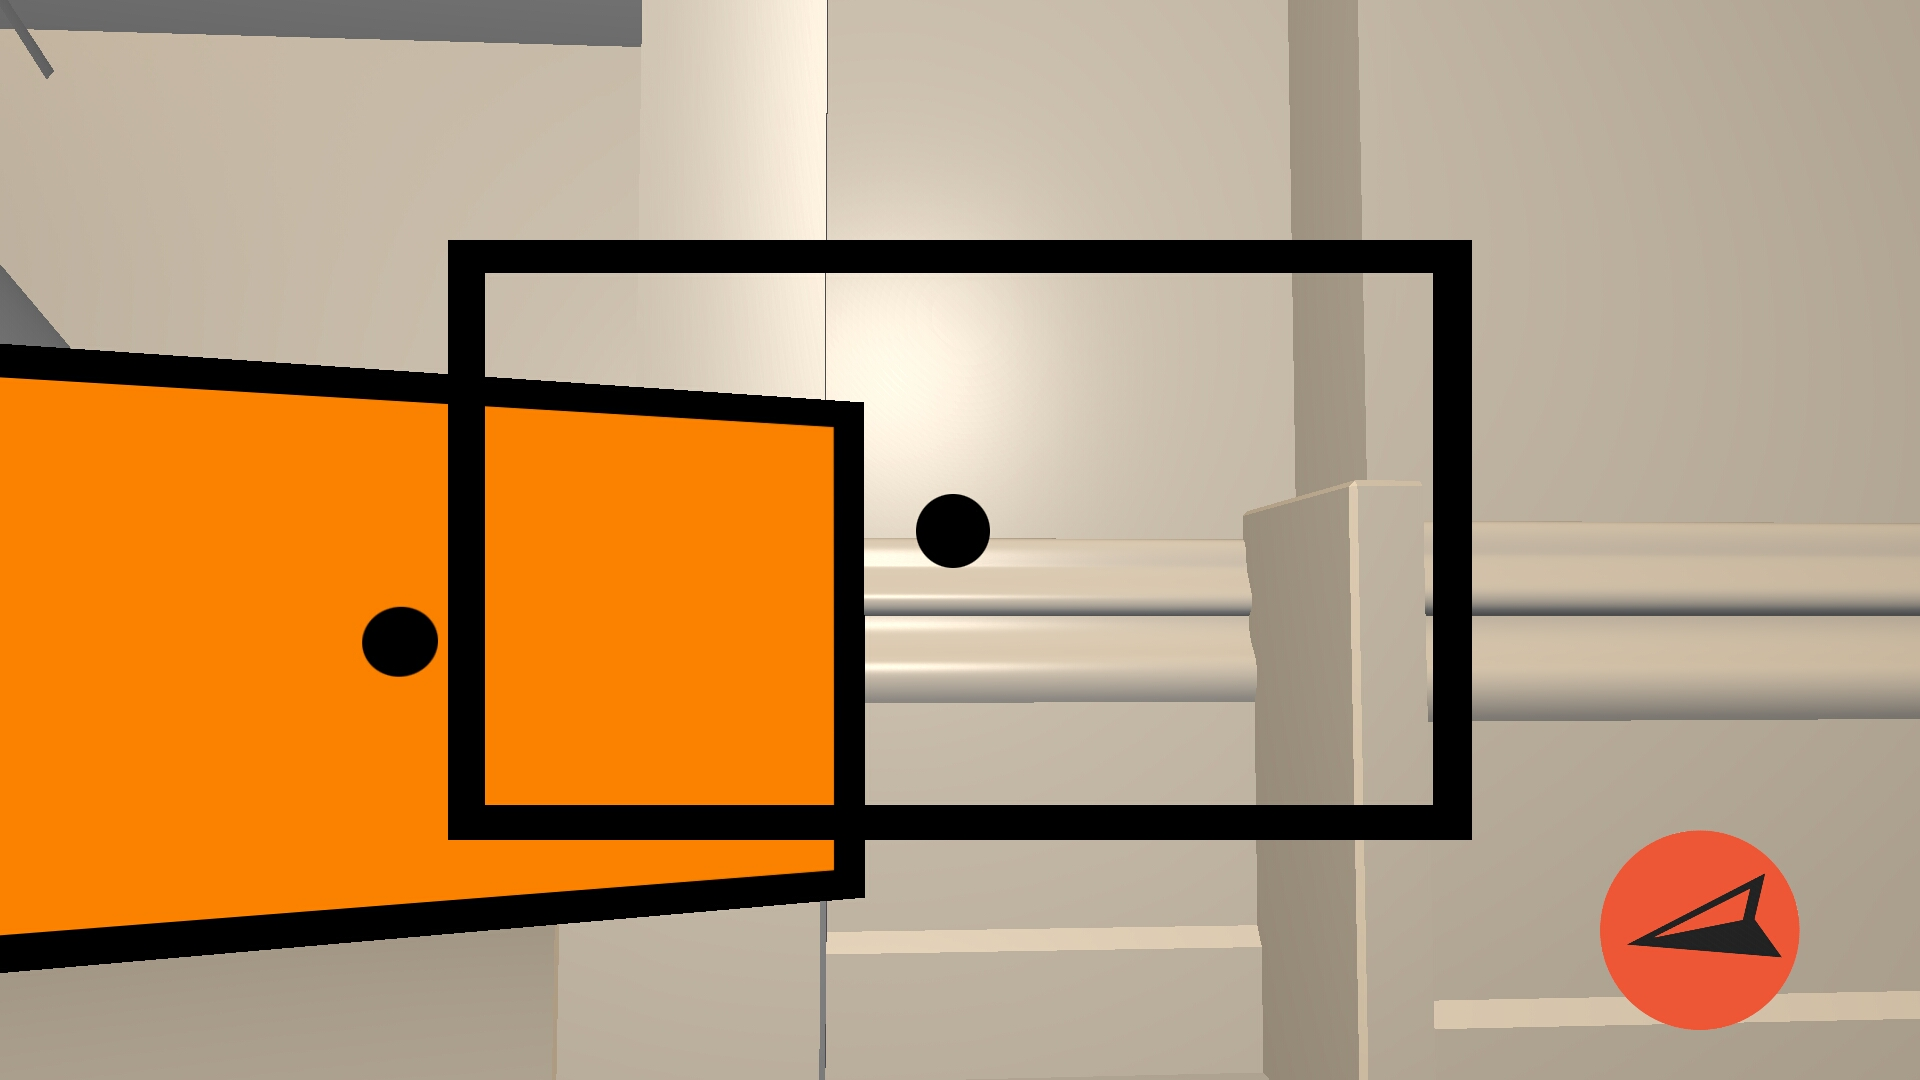
\includegraphics[width=0.49\columnwidth]{figures/user_study_screen_shot1.jpg}}
	\subfigure[Sub-task of recognition]{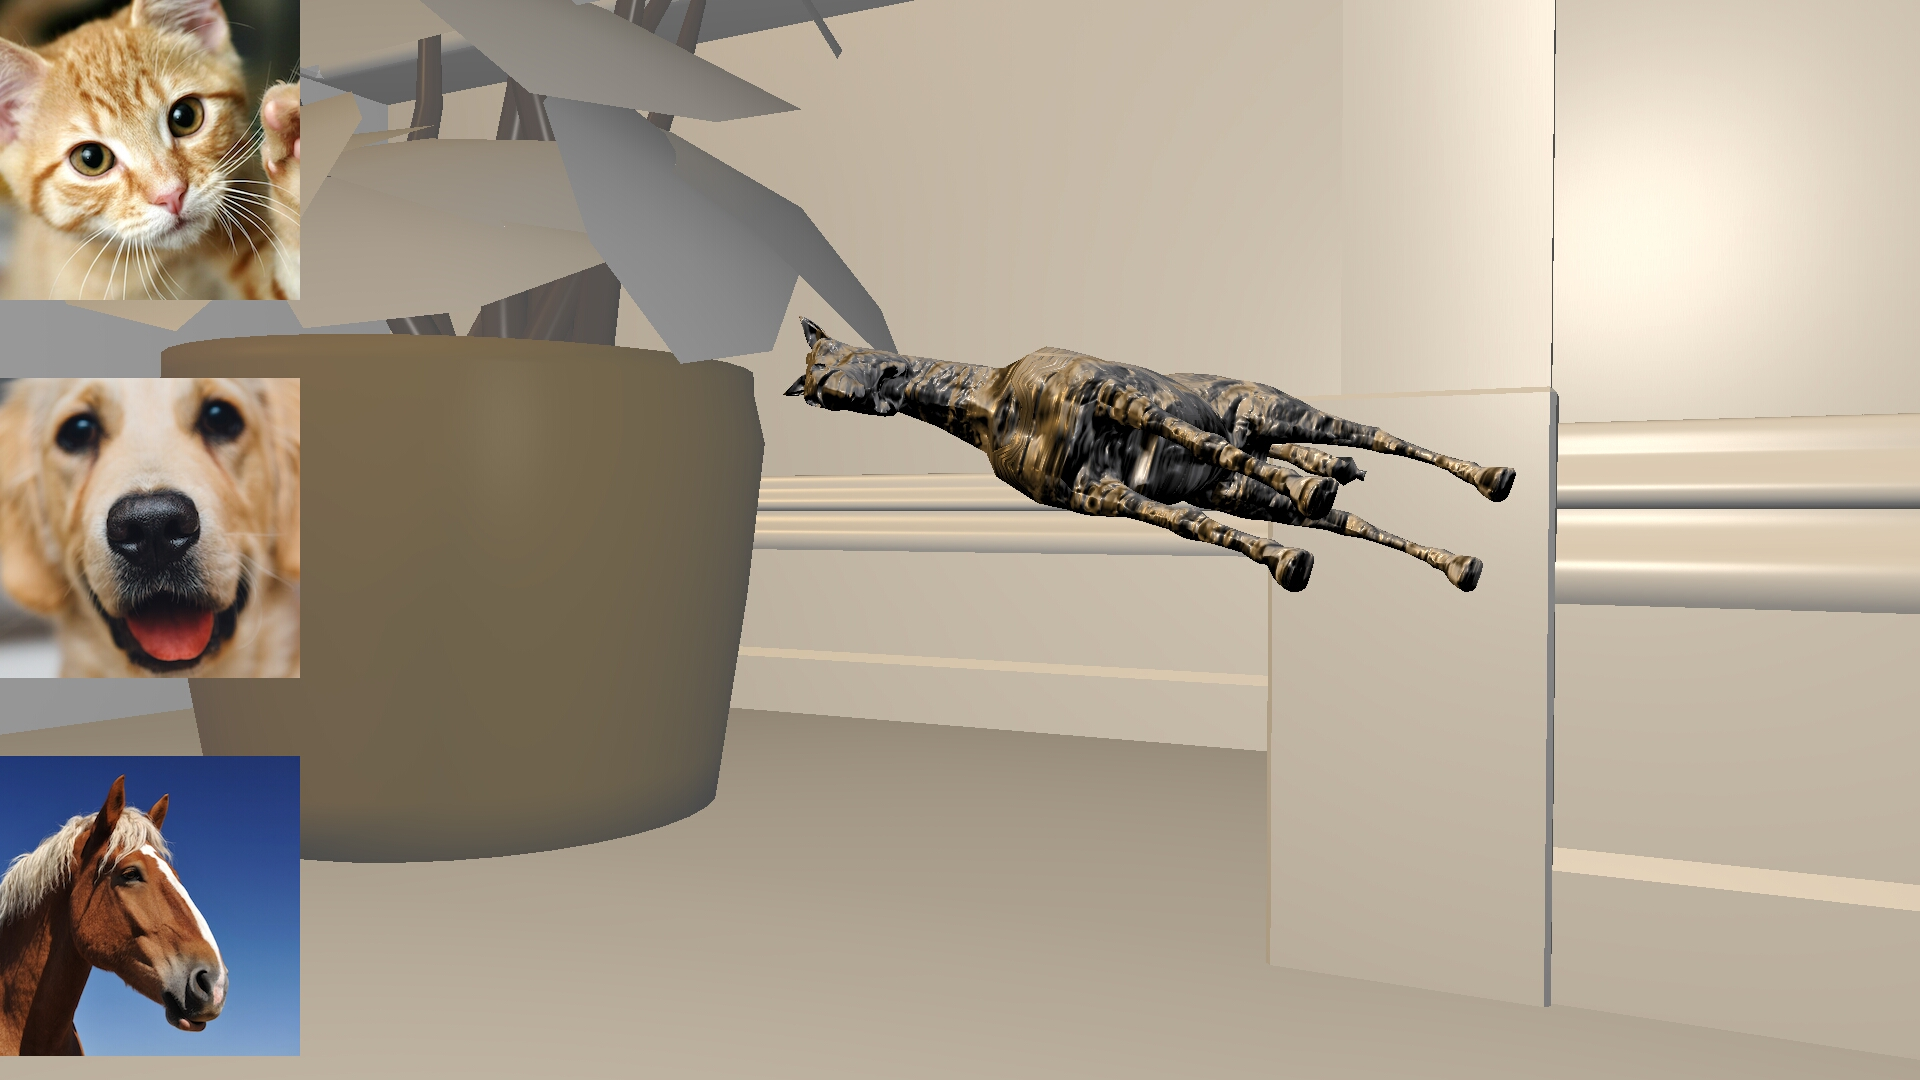
\includegraphics[width=0.49\columnwidth]{figures/user_study_screen_shot2.jpg}}
	\caption{Screenshots of the test application. During one run of the test application, the two sub-tasks are repeated ten times with different animal models. (a) Sub-task of navigation. In the test application, users need to pan and tilt to align the camera viewfinder with the orange plate by following the direction of the compass. If there exist network delay and jitter, users will feel them when panning and tilting. (b) Sub-task of recognition. After aligning the camera viewfinder with the plate, an object appears. The object is not static, but rotating and moving around instead. As similar to the sub-task of navigation, the movement and rotation of the object is also influenced by network delay and jitter.}
	\label{fig:us}
\end{figure}

\subsubsection{Results}
\label{sec:hrr:us:ms:r}

To understand how each factor affects the SDoT and the ODoT, we use analysis of variance (ANOVA) to interpret our experimental data.

We use a four-way ANOVA test to investigate the effect of all four factors. However the factor combination of delay and jitter is not complete, since jitter is not applicable when the delay is $0\mathrm{ms}$. So we exclude the delay level $0\mathrm{ms}$ in the four-way ANOVA test.
As shown in Table~\ref{tab:fal}, the four-way ANOVA considers the four factors and their levels, except for $0\mathrm{ms}$ of delay.

We also analyze the effect of the delay factor and its interaction with key model fidelity and environment model fidelity. For this analysis, we resort to a three-way ANOVA for the combination of delay, key model fidelity and environment model fidelity. Table~\ref{tab:fal} shows the factors of the three way ANOVA.

\begin{table}[!htbp]
\caption{Factors and levels of the ANOVA tests.}
\label{tab:fal}
\begin{tabular}{llllllllll}
\hline\noalign{\smallskip}
& \multicolumn{2}{c}{\makecell{Key Model\\Fidelity}} & \multicolumn{2}{c}{\makecell{Environment\\Model\\Fidelity}} & \multicolumn{3}{c}{Delay} & \multicolumn{2}{c}{Jitter} \\
\noalign{\smallskip}\hline\noalign{\smallskip}
& Low & High & Low & High & $0\mathrm{ms}$ & $80\mathrm{ms}$ & $120\mathrm{ms}$ & applied & not applied \\
\noalign{\smallskip}\hline\noalign{\smallskip}
Four-way ANOVA & \cmark & \cmark & \cmark & \cmark & \xmark & \cmark & \cmark & \cmark & \cmark \\
Three-way ANOVA & \cmark & \cmark & \cmark & \cmark & \cmark & \cmark & \cmark & \xmark & \xmark \\
\noalign{\smallskip}\hline
\end{tabular}
\end{table}

Table~\ref{tab:mou} shows the grand mean of the ODoT measure for all factors. The ODoT refers to the number of objects the user did not recognize, hence higher scores represent higher objective difficulty of task. Since we employ two tests of significance (four-way and a three-way ANOVA) we calculate two grand means of the ODoT for each factor level. Four-way ANOVA does not consider the results of configurations 1 to 4 of Table~\ref{tab:pus} (since it does not consider $0\mathrm{ms}$ delay as previously explained). Table~\ref{tab:mou} shows that the ODoT varies with different levels of each factor. However, not all factors have an effect on the ODoT.
We can see that in both, the four-way and the three-way ANOVA, participants are able to reduce the number of incorrectly recognized objects with high-fidelity key models and in low-fidelity environment models.
% and jitter.
The grand means for the factor delay do not agree in the four-way ANOVA and the three-way ANOVA, so we consider the factor delay as not having an effect on ODoT.

Table~\ref{tab:mom} shows the grand means with respect to SDoT. As in Table~\ref{tab:mou}, we show the grand means calculated for the four-way ANOVA and three-way ANOVA tests in Table~\ref{tab:mom}. The means are measured through a 5 point Likert Scale, where larger values indicate higher subjective difficulty of task.

From Table~\ref{tab:mom}, we can see that three factors have effects on the SDoT. The SDoT is reduced for high-fidelity key models and low delay.
% and jitter.
The grand means for the factor environment model fidelity do not agree in the four-way ANOVA and the three-way ANOVA, so we cannot conclude that the factor environment model fidelity has an effect on SDoT.

\begin{table}[!htbp]
\caption{Grand means of the ODoT for each factor.}
\label{tab:mou}
\begin{tabular}{llllllllll}
\hline\noalign{\smallskip}
& \multicolumn{2}{c}{\makecell{Key Model\\Fidelity}} & \multicolumn{2}{c}{\makecell{Environment\\Model\\Fidelity}} & \multicolumn{3}{c}{Delay} & \multicolumn{2}{c}{Jitter} \\
\noalign{\smallskip}\hline\noalign{\smallskip}
& low & high & low & high & $0\mathrm{ms}$ & $80\mathrm{ms}$ & $120\mathrm{ms}$ & applied & not applied \\
\noalign{\smallskip}\hline\noalign{\smallskip}
Four-way ANOVA & 4.6 & 3.5 & 3.9 & 4.2 & - & 4.0 & 4.1 & 3.8 & 4.2 \\
Three-way ANOVA & 4.3 & 3.5 & 3.8 & 4.0 & 4.0 & 3.9 & 3.8 & - & - \\
\noalign{\smallskip}\hline
\end{tabular}
\end{table}

\begin{table}[!htbp]
\caption{Grand means of the SDoT for each factor.}
\label{tab:mom}
\begin{tabular}{llllllllll}
\hline\noalign{\smallskip}
& \multicolumn{2}{c}{\makecell{Key Model\\Fidelity}} & \multicolumn{2}{c}{\makecell{Environment\\Model\\Fidelity}} & \multicolumn{3}{c}{Delay} & \multicolumn{2}{c}{Jitter} \\
\noalign{\smallskip}\hline\noalign{\smallskip}
& low & high & low & high & $0\mathrm{ms}$ & $80\mathrm{ms}$ & $120\mathrm{ms}$ & applied & not applied \\
\noalign{\smallskip}\hline\noalign{\smallskip}
Four-way ANOVA & 2.7 & 2.5 & 2.7 & 2.6 & - & 2.5 & 2.8 & 2.5 & 2.7 \\
Three-way ANOVA & 2.4 & 2.2 & 2.2 & 2.3 & 1.9 & 2.4 & 2.6 & - & - \\
\noalign{\smallskip}\hline
\end{tabular}
\end{table}

However, the conclusions drawn from Tables~\ref{tab:mou} and \ref{tab:mom} may not be significantly different in statistics.
% It is probably caused by the small number of samples. 
Hence, we analyze the variance for both metrics, i.e. ODoT and SDoT, to determine whether any of the differences between the means are statistically significant, and compare the $p$-values to a significance level to decide whether the $p$-value suggests accept or reject on the null hypothesis. We choose a significance level of 0.05.

Tables~\ref{tab:fau} and \ref{tab:tau} demonstrate the results of ANOVA in terms of the ODoT, where Table~\ref{tab:fau} shows the results of the four way ANOVA while Table~\ref{tab:tau} shows the results of the three way ANOVA.

Only the key model fidelity factor exhibits a $p$-value less than 0.05 for both ANOVA tests for the ODoT measure.
To explore the interaction between a factor pair or among multiple factors, we also calculate the $p$-values for those interactions.
These kinds of calculations are performed for every combination of factors, including combination of two factors, combination of three factors, and combination of four factors if plausible.
From Tables~\ref{tab:fau} and \ref{tab:tau}, we can see that there is no combination whose $p$-value is smaller than 0.05.
This indicates that these factors are independent from each other in terms of the ODoT.

\begin{table}[!htbp]
\caption{Four-way ANOVA of the ODoT.}
\label{tab:fau}
\begin{tabular}{lll}
\hline\noalign{\smallskip}
Source & F-statistics & $p$-value \\
\noalign{\smallskip}\hline\noalign{\smallskip}
Key Model Fidelity & 14.9 & 0.0001 \\
Environment Model Fidelity & 1.28 & 0.2589 \\
Delay & 0.14 & 0.7063 \\
Jitter & 1.71 & 0.1929 \\
Key Model Fidelity $\times$ Environment Model Fidelity & 0 & 0.9769 \\
Key Model Fidelity $\times$ Delay & 0.14 & 0.7063 \\
Key Model Fidelity $\times$ Jitter & 0.24 & 0.6223 \\
Environment Model Fidelity $\times$ Delay & 0.24 & 0.6223 \\
Environment Model Fidelity $\times$ Jitter & 1.03 & 0.3109 \\
Delay $\times$ Jitter & 0.53 & 0.4689 \\
Key Model Fidelity $\times$ Environment Model Fidelity $\times$ Delay & 2.93 & 0.0882 \\
Key Model Fidelity $\times$ Environment Model Fidelity $\times$ Jitter & 0.37 & 0.5429 \\
Key Model Fidelity $\times$ Delay $\times$ Jitter & 0.04 & 0.8392 \\
Environment Model Fidelity $\times$ Delay $\times$ Jitter & 3.13 & 0.0781 \\
Key Model Fidelity $\times$ Environment Model Fidelity $\times$ Delay $\times$ Jitter & 1.28 & 0.2589 \\
\noalign{\smallskip}\hline
\end{tabular}
\end{table}

\begin{table}[!htbp]
\caption{Three-way ANOVA of the ODoT.}
\label{tab:tau}
\begin{tabular}{lll}
\hline\noalign{\smallskip}
Source & F-statistics & $p$-value \\
\noalign{\smallskip}\hline\noalign{\smallskip}
Key Model Fidelity & 6.33 & 0.0128 \\
Environment Model Fidelity & 0.12 & 0.7342 \\
Delay & 0.12 & 0.8826 \\
Key Model Fidelity $\times$ Environment Model Fidelity & 004 & 0.8385 \\
Key Model Fidelity $\times$ Delay & 0.28 & 0.7544 \\
Environment Model Fidelity $\times$ Delay & 0.48 & 0.6217 \\
Key Model Fidelity $\times$ Environment Model Fidelity $\times$ Delay & 0.6 & 0.5517 \\
\noalign{\smallskip}\hline
\end{tabular}
\end{table}

Table~\ref{tab:fam} shows the results of four-way ANOVA for the SDoT measure, and Table~\ref{tab:tam} shows the results of three-way ANOVA test.
As opposed to the tests of significance for the ODoT measure, for the SDoT, the key model fidelity is not significant. Instead, the delay factor is statistically significant (with a $p$-value of 0.0281 for the four-way ANOVA test and 0.0018 for the three-way ANOVA test).

Furthermore, we analyze the interaction for factor combinations (just like what we did for the ODoT measure).
The results demonstrate that there is no interaction among the four factors.

\begin{table}[!htbp]
\caption{Four-way ANOVA of SDoT.}
\label{tab:fam}
\begin{tabular}{llllll}
\hline\noalign{\smallskip}
Source & F-statistics & $p$-value \\
\noalign{\smallskip}\hline\noalign{\smallskip}
Key Model Fidelity & 2.95 & 0.0871 \\
Environment Model Fidelity & 0.96 & 0.3271 \\
Delay & 4.88 & 0.0281 \\
Jitter & 2.95 & 0.0871 \\
Key Model Fidelity $\times$ Environment Model Fidelity & 0.38 & 0.54 \\
Key Model Fidelity $\times$ Delay & 0.02 & 0.9024 \\
Key Model Fidelity $\times$ Jitter & 0.38 & 0.54 \\
Environment Model Fidelity $\times$ Delay & 1.22 & 0.2704 \\
Environment Model Fidelity $\times$ Jitter & 1.82 & 0.1783 \\
Delay $\times$ Jitter & 0.74 & 0.3911 \\
Key Model Fidelity $\times$ Environment Model Fidelity $\times$ Delay & 0.24 & 0.6239 \\
Key Model Fidelity $\times$ Environment Model Fidelity $\times$ Jitter & 0.54 & 0.4622 \\
Key Model Fidelity $\times$ Delay $\times$ Jitter & 0.54 & 0.4622 \\
Environment Model Fidelity $\times$ Delay $\times$ Jitter & 2.95 & 0.0871 \\
Key Model Fidelity $\times$ Environment Model Fidelity $\times$ Delay $\times$ Jitter & 3.39 & 0.0669 \\
\noalign{\smallskip}\hline
\end{tabular}
\end{table}

\begin{table}[!htbp]
\caption{Three-way ANOVA of SDoT.}
\label{tab:tam}
\begin{tabular}{llllll}
\hline\noalign{\smallskip}
Source & F-statistics & $p$-value \\
\noalign{\smallskip}\hline\noalign{\smallskip}
Key Model Fidelity & 1.2 & 0.2743 \\
Environment Model Fidelity & 0.34 & 0.5623 \\
Delay & 6.55 & 0.0018 \\
Key Model Fidelity $\times$ Environment Model Fidelity & 0.04 & 0.8468 \\
Key Model Fidelity $\times$ Delay & 0.7 & 0.4964 \\
Environment Model Fidelity $\times$ Delay & 0.16 & 0.8503 \\
Key Model Fidelity $\times$ Environment Model Fidelity $\times$ Delay & 0.46 & 0.6309 \\
\noalign{\smallskip}\hline
\end{tabular}
\end{table}

Given the results obtained with the tests of significance, we conclude that the key model fidelity factor affects the ODoT significantly, while the delay factor affects the SDoT significantly. We could not show any influence of other factors beyond what may occur by chance. We summarize our results in Table~\ref{tab:hypo}.
% by suggesting either accept or reject on each null hypothesis.
H\textsubscript{01} and H\textsubscript{07} are rejected since the key model fidelity and delay factors have a significant effect on ODoT and SDoT respectively.

\begin{table}[!htbp]
\caption{Hypotheses. The third column shows if a hypothesis is accepted or rejected according to our ANOVA analysis.}
\label{tab:results}
\begin{tabular}{lll}
\hline\noalign{\smallskip}
H\textsubscript{01} & Different model fidelities do not affect the ODoT & reject \\
H\textsubscript{02} & Different environment fidelities do not affect the ODoT & accept \\
H\textsubscript{03} & Different network delays do not affect the ODoT & accept \\
H\textsubscript{04} & Existence of jitter does not affect the ODoT & accept \\
H\textsubscript{05} & Different model fidelities do not affect the SDoT & accept \\
H\textsubscript{06} & Different environment fidelities do not affect the SDoT & accept \\
H\textsubscript{07} & Different network delays do not affect the SDoT & reject \\
H\textsubscript{08} & Existence of jitter does not affect the SDoT & accept \\
\noalign{\smallskip}\hline
\end{tabular}
\end{table}

Now we can answer the four questions asked at the beginning of this section.
\begin{enumerate}
\item
The key model fidelity has a significant effect on the ODoT. Greater key model fidelity helps the user to achieve better recognition. However, we could not show a significant effect on the SDoT. 
\item
We could not show a significant effect of  environment fidelity on either the ODoT or the SDoT.
\item
The delay factor has a significant effect on the SDoT. A longer delay results in a higher SDoT. It did not have a significant effect on the ODoT.
\item
We could not show a significant effect of jitter on either the ODoT or the SDoT in our study.
\end{enumerate}

In conclusion, our user study supports the idea of only rendering and sending key models in remote rendering applications.
Based on an analysis of the variance of both, ODoT and SDoT, we found that key model fidelity is the only factor that has a statistically significant effect on ODoT, and that delay is the only factor that has a statistically significant effect on SDoT.
Thus, our application design is well informed to address the overall DoT by addressing the factors key model fidelity and delay, which are the two factors that have significant effects.
To minimize the network delay, we reduce the environment model fidelity. The user study indicates that this reduction is not likely to affect the SDoT.
Moreover, since the factor key model fidelity has a significant effect on ODoT, our method maintains the fidelity of the key model.

\section{Conclusions}
\label{sec:hrr:c}

We propose a hybrid remote rendering framework for mobile applications.
It uses a client-server model, where the server is responsible for rendering high-fidelity models, encoding and sending the rendered frames to the client. However, in our approach, only key models are rendered on the server and sent to the client. The client uses low-fidelity models to render frames locally and overlays the frames received from the server onto its local rendering frames.
In this way, the client is able to display rendering effects that are not available with mobile graphic devices, with lower bandwidth requirements than in streaming-only solutions.

We conducted a user study on the factors involved in the proposed framework affecting the ODoT and the SDoT: key model fidelity, environment model fidelity, delay and jitter. We developed an experimental application in which users are asked to recognize objects in different configurations pertaining to the identified factors. Our user study shows that the key model fidelity affects the ODoT and that network delay plays an important role in the SDoT. When streaming over non-dedicated networks, the conditions often do not satisfy the requirements of remote rendering applications. Therefore, trading off between rendering quality and network delay is essential, but existing remote rendering applications cannot address this issue in a satisfactory way. The most important contribution of the proposed framework is enabling such a trade-off.

%======================================================================
\chapter{Conclusion}
\label{chap:c}
%======================================================================

Augmented reality is an emerging direction in industry and research, which has broad use in various fields, e.g. games, communication, medicine and training. We focus on the use of AR in the area of training in this proposal. Manufacturers, such as Boeing, have already leveraged the advantages of augmented reality in their training department~\cite{caudell1992}. Great improvements have been made by using AR compared to traditional training.

However, there are two disadvantages with the existing AR training systems, as discussed in Chapter~\ref{chap:bg}.
One one hand, the existing AR training systems are designed as task-specific. Therefore, it is difficult to adapt them for a new task.
On the other hand, the existing AR training systems are one-way, namely, the trainees obtain guidance from the trainer who authored the guide without real-time feedback on their performance.

We propose a novel framework for augmented reality training.
It has three main contributions:
\begin{itemize}
  \item
  We propose a method that allows the trainer to author guidances in real-time.
  \item
  We propose a method that enables the trainer to collect feedbacks from the trainees during the training process in real-time.
  \item
  We propose a method that makes the AR training framework work with consumer-level devices without dedicated hardware such as powerful graphics.
\end{itemize}

The framework contains five parts: 1) video capture; 2) video object segmentation; 3) pose estimation; 4) remote rendering; 5) synchronization.
Among the five parts, we identify the three parts that we need to propose our own solutions: 1) video object segmentation; 2) remote rendering; 3) synchronization.

The method of video object segmentation is presented in Section~\ref{chap:vos}, which is used in the real-time object pose tracking system.
The proposed method is fully automatic, fast, and does not make restrictive assumptions about object motions.
In experiments on standard data sets, the proposed approach achieves comparable results to state-of-the-art video object segmentation methods, but our method is much faster.
It is an essential building block in a real-time region-based object pose tracking system.
We also demonstrate an application of the proposed method to content-aware video compression.

The work of remote rendering method is presented in Section~\ref{chap:hrr}.
Although the field of remote rendering has been studied for decades and the implementations have been used in many areas, such as gaming and virtual tour, researchers primarily focused on remote rendering of the entire frame.
We pay attention on the importance of models. In other words, we render object with higher importance with high-fidelity models, and render objects with lower importance with low-fidelity models.
It enables a trade-off between rendering quality and network delay.

The remaining work includes the implementation of the communication schema and the integration of all parts into one framework. which is described in Section~\ref{chap:dm}.

\section{Schedule}
\label{sec:c:s}

The following schedule is given in terms of the estimated time required following the completion of this proposal.

\textbf{Mar. to Apr. 2018 (2 months)}: Implement the proposed pose estimation algorithm that uses the video object segmentation method described in Chapter~\ref{chap:vos}.

\textbf{May to Jul. 2018 (3 months)}: 1) Implement the communication schema and integrate all parts into one framework. 2) Design the user study and submit the application to the Research Ethics Board (REB) at the University of Ottawa.

\textbf{Aug. 2018 (1 month)}: Prepare the user study and wait for the approval of the user study from REB.

\textbf{Sept. 2018 (1 month)} Conduct the user study.

\textbf{Oct. 2018 to Dec. 2018 (3 months)}: Finishing writing thesis.


%----------------------------------------------------------------------
% APPENDICES
%---------------------------------------------------------------------- 
%\appendix
% Designate with \appendix declaration which just changes numbering style 
% from here on
% Add a title page before the appendices and a line in the Table of Contents
%\chapter*{APPENDICES}
%\addcontentsline{toc}{chapter}{APPENDICES} 
%
%% An appendix
%======================================================================
\chapter{Sources of Information and Help}
\label{ch:Appendix-Sources-of-Info}
%======================================================================
The best source of information about \LaTeX\ is the two books mentioned in this course \cite{lamport.book,goossens.book}.
Another excellent resource is the UseNet newsgroup \verb=comp.text.tex=.
A frequently-asked-questions (FAQ) list is also maintained by this news group.
You might also search the World Wide Web for ``LaTeX'' for other sources of help.
 %"Sources of Information and Help"
%% An appendix
%======================================================================
\chapter[PDF Plots From Matlab]{Matlab Code for Making a PDF Plot}
\label{ch:Appendix-Matlab} 
%======================================================================
\section{Using the GUI}
Properties of Matab plots can be adjusted from the plot window via a graphical interface. Under the Desktop menu in the Figure window, select the Property Editor. You may also want to check the Plot Browser and Figure Palette for more tools. To adjust properties of the axes, look under the Edit menu and select Axes Properties.

To set the figure size and to save as PDF or other file formats, click the Export Setup button in the figure Property Editor.

\section{From the Command Line} 
All figure properties can also be manipulated from the command line. Here's an example: 
\begin{verbatim}
x=[0:0.1:pi];
hold on % Plot multiple traces on one figure
plot(x,sin(x))
plot(x,cos(x),'--r')
plot(x,tan(x),'.-g')
title('Some Trig Functions Over 0 to \pi') % Note LaTeX markup!
legend('{\it sin}(x)','{\it cos}(x)','{\it tan}(x)')
hold off
set(gca,'Ylim',[-3 3]) % Adjust Y limits of "current axes"
set(gcf,'Units','inches') % Set figure size units of "current figure"
set(gcf,'Position',[0,0,6,4]) % Set figure width (6 in.) and height (4 in.)
cd n:\thesis\plots % Select where to save
print -dpdf plot.pdf % Save as PDF
\end{verbatim}  %"Matlab Code for Making a PDF Plot"

%----------------------------------------------------------------------
% END MATERIAL
%----------------------------------------------------------------------

% B I B L I O G R A P H Y
% -----------------------
%
% The following statement selects the style to use for references.  It controls the sort order of the entries in the bibliography and also the formatting for the in-text labels.
\bibliographystyle{plain}
% This specifies the location of the file containing the bibliographic information.  
% It assumes you're using BibTeX (if not, why not?).
\ifthenelse{\boolean{PrintVersion}}{
\cleardoublepage % This is needed if the book class is used, to place the anchor in the correct page,
                 % because the bibliography will start on its own page.
}{
\clearpage       % Use \clearpage instead if the document class uses the "oneside" argument
}
\phantomsection  % With hyperref package, enables hyperlinking from the table of contents to bibliography             
% The following statement causes the title "References" to be used for the bibliography section:
\renewcommand*{\bibname}{References}

% Add the References to the Table of Contents
\addcontentsline{toc}{chapter}{\textbf{References}}

\bibliography{bibliography/IEEEabrv,bibliography/abrv,bibliography/ref,bibliography/os_ref,bibliography/rr_ref}
% Tip 5: You can create multiple .bib files to organize your references. 
% Just list them all in the \bibliogaphy command, separated by commas (no spaces).


%----------------------------------------------------------------------
\end{document}
%======================================================================



%%% Local Variables: 
%%% mode: latex
%%% TeX-master: t
%%% End: 
